\documentclass[11pt,]{article}
\usepackage[left=1in,top=1in,right=1in,bottom=1in]{geometry}
\newcommand*{\authorfont}{\fontfamily{phv}\selectfont}
\usepackage[]{mathpazo}


  \usepackage[T1]{fontenc}
  \usepackage[utf8]{inputenc}




\usepackage{abstract}
\renewcommand{\abstractname}{}    % clear the title
\renewcommand{\absnamepos}{empty} % originally center

\renewenvironment{abstract}
 {{%
    \setlength{\leftmargin}{0mm}
    \setlength{\rightmargin}{\leftmargin}%
  }%
  \relax}
 {\endlist}

\makeatletter
\def\@maketitle{%
  \newpage
%  \null
%  \vskip 2em%
%  \begin{center}%
  \let \footnote \thanks
    {\fontsize{18}{20}\selectfont\raggedright  \setlength{\parindent}{0pt} \@title \par}%
}
%\fi
\makeatother




\setcounter{secnumdepth}{0}

\usepackage{color}
\usepackage{fancyvrb}
\newcommand{\VerbBar}{|}
\newcommand{\VERB}{\Verb[commandchars=\\\{\}]}
\DefineVerbatimEnvironment{Highlighting}{Verbatim}{commandchars=\\\{\}}
% Add ',fontsize=\small' for more characters per line
\usepackage{framed}
\definecolor{shadecolor}{RGB}{248,248,248}
\newenvironment{Shaded}{\begin{snugshade}}{\end{snugshade}}
\newcommand{\AlertTok}[1]{\textcolor[rgb]{0.94,0.16,0.16}{#1}}
\newcommand{\AnnotationTok}[1]{\textcolor[rgb]{0.56,0.35,0.01}{\textbf{\textit{#1}}}}
\newcommand{\AttributeTok}[1]{\textcolor[rgb]{0.77,0.63,0.00}{#1}}
\newcommand{\BaseNTok}[1]{\textcolor[rgb]{0.00,0.00,0.81}{#1}}
\newcommand{\BuiltInTok}[1]{#1}
\newcommand{\CharTok}[1]{\textcolor[rgb]{0.31,0.60,0.02}{#1}}
\newcommand{\CommentTok}[1]{\textcolor[rgb]{0.56,0.35,0.01}{\textit{#1}}}
\newcommand{\CommentVarTok}[1]{\textcolor[rgb]{0.56,0.35,0.01}{\textbf{\textit{#1}}}}
\newcommand{\ConstantTok}[1]{\textcolor[rgb]{0.00,0.00,0.00}{#1}}
\newcommand{\ControlFlowTok}[1]{\textcolor[rgb]{0.13,0.29,0.53}{\textbf{#1}}}
\newcommand{\DataTypeTok}[1]{\textcolor[rgb]{0.13,0.29,0.53}{#1}}
\newcommand{\DecValTok}[1]{\textcolor[rgb]{0.00,0.00,0.81}{#1}}
\newcommand{\DocumentationTok}[1]{\textcolor[rgb]{0.56,0.35,0.01}{\textbf{\textit{#1}}}}
\newcommand{\ErrorTok}[1]{\textcolor[rgb]{0.64,0.00,0.00}{\textbf{#1}}}
\newcommand{\ExtensionTok}[1]{#1}
\newcommand{\FloatTok}[1]{\textcolor[rgb]{0.00,0.00,0.81}{#1}}
\newcommand{\FunctionTok}[1]{\textcolor[rgb]{0.00,0.00,0.00}{#1}}
\newcommand{\ImportTok}[1]{#1}
\newcommand{\InformationTok}[1]{\textcolor[rgb]{0.56,0.35,0.01}{\textbf{\textit{#1}}}}
\newcommand{\KeywordTok}[1]{\textcolor[rgb]{0.13,0.29,0.53}{\textbf{#1}}}
\newcommand{\NormalTok}[1]{#1}
\newcommand{\OperatorTok}[1]{\textcolor[rgb]{0.81,0.36,0.00}{\textbf{#1}}}
\newcommand{\OtherTok}[1]{\textcolor[rgb]{0.56,0.35,0.01}{#1}}
\newcommand{\PreprocessorTok}[1]{\textcolor[rgb]{0.56,0.35,0.01}{\textit{#1}}}
\newcommand{\RegionMarkerTok}[1]{#1}
\newcommand{\SpecialCharTok}[1]{\textcolor[rgb]{0.00,0.00,0.00}{#1}}
\newcommand{\SpecialStringTok}[1]{\textcolor[rgb]{0.31,0.60,0.02}{#1}}
\newcommand{\StringTok}[1]{\textcolor[rgb]{0.31,0.60,0.02}{#1}}
\newcommand{\VariableTok}[1]{\textcolor[rgb]{0.00,0.00,0.00}{#1}}
\newcommand{\VerbatimStringTok}[1]{\textcolor[rgb]{0.31,0.60,0.02}{#1}}
\newcommand{\WarningTok}[1]{\textcolor[rgb]{0.56,0.35,0.01}{\textbf{\textit{#1}}}}
\usepackage{longtable,booktabs}

\usepackage{graphicx,grffile}
\makeatletter
\def\maxwidth{\ifdim\Gin@nat@width>\linewidth\linewidth\else\Gin@nat@width\fi}
\def\maxheight{\ifdim\Gin@nat@height>\textheight\textheight\else\Gin@nat@height\fi}
\makeatother
% Scale images if necessary, so that they will not overflow the page
% margins by default, and it is still possible to overwrite the defaults
% using explicit options in \includegraphics[width, height, ...]{}
\setkeys{Gin}{width=\maxwidth,height=\maxheight,keepaspectratio}


\title{An Analysis of Suicides Around the World  }



\author{\Large Joshua D. Ingram\vspace{0.05in} \newline\normalsize\emph{New College of Florida}  }


\date{}

\usepackage{titlesec}

\titleformat*{\section}{\normalsize\bfseries}
\titleformat*{\subsection}{\normalsize\itshape}
\titleformat*{\subsubsection}{\normalsize\itshape}
\titleformat*{\paragraph}{\normalsize\itshape}
\titleformat*{\subparagraph}{\normalsize\itshape}


\usepackage{natbib}
\bibliographystyle{apsr}
\usepackage[strings]{underscore} % protect underscores in most circumstances



\newtheorem{hypothesis}{Hypothesis}
\usepackage{setspace}


% set default figure placement to htbp
\makeatletter
\def\fps@figure{htbp}
\makeatother


% move the hyperref stuff down here, after header-includes, to allow for - \usepackage{hyperref}

\makeatletter
\@ifpackageloaded{hyperref}{}{%
\ifxetex
  \PassOptionsToPackage{hyphens}{url}\usepackage[setpagesize=false, % page size defined by xetex
              unicode=false, % unicode breaks when used with xetex
              xetex]{hyperref}
\else
  \PassOptionsToPackage{hyphens}{url}\usepackage[draft,unicode=true]{hyperref}
\fi
}

\@ifpackageloaded{color}{
    \PassOptionsToPackage{usenames,dvipsnames}{color}
}{%
    \usepackage[usenames,dvipsnames]{color}
}
\makeatother
\hypersetup{breaklinks=true,
            bookmarks=true,
            pdfauthor={Joshua D. Ingram (New College of Florida)},
             pdfkeywords = {Suicides, multiple regression, bootsrapping},  
            pdftitle={An Analysis of Suicides Around the World},
            colorlinks=true,
            citecolor=blue,
            urlcolor=blue,
            linkcolor=magenta,
            pdfborder={0 0 0}}
\urlstyle{same}  % don't use monospace font for urls

% Add an option for endnotes. -----


% add tightlist ----------
\providecommand{\tightlist}{%
\setlength{\itemsep}{0pt}\setlength{\parskip}{0pt}}

% add some other packages ----------

% \usepackage{multicol}
% This should regulate where figures float
% See: https://tex.stackexchange.com/questions/2275/keeping-tables-figures-close-to-where-they-are-mentioned
\usepackage[section]{placeins}


\begin{document}
	
% \pagenumbering{arabic}% resets `page` counter to 1 
%
% \maketitle

{% \usefont{T1}{pnc}{m}{n}
\setlength{\parindent}{0pt}
\thispagestyle{plain}
{\fontsize{18}{20}\selectfont\raggedright 
\maketitle  % title \par  

}

{
   \vskip 13.5pt\relax \normalsize\fontsize{11}{12} 
\textbf{\authorfont Joshua D. Ingram} \hskip 15pt \emph{\small New College of Florida}   

}

}








\begin{abstract}

    \hbox{\vrule height .2pt width 39.14pc}

    \vskip 8.5pt % \small 

\noindent This document contains an overview of suicides around the world with
both demographic and the aggregate analysis.


\vskip 8.5pt \noindent \emph{Keywords}: Suicides, multiple regression, bootsrapping \par

    \hbox{\vrule height .2pt width 39.14pc}



\end{abstract}


\vskip -8.5pt


 % removetitleabstract

\noindent  

\hypertarget{data-wrangling}{%
\section{Data Wrangling}\label{data-wrangling}}

After removing some variables that will not be used in the analysis,
5.81\% of our values our missing. Of this, HDI has 69.93\% missing
values in the column.

I created 2 new categorical variables, Region and Development. Region is
split up into 8 regions around the world (as determined by Homeland
Security): Africa, Asia, Caribbean, Central America, Europe, North
America, Oceania, South America. Development has 4 ordered levels: high
(HDI \textgreater= .8), medium ( .6 \textless= HDI \textless= .799), low
or very low (HDI \textless= .599) and unknown (HDI is missing). An
unknown category was created because there is the potential that there
could be some relationship with HDI being unkown and the development
level for a country\ldots{} especially considering the amount of missing
data in HDI. Since HDI wasn't invented until 1990, I removed the years
1985-1989. So the data only contains information on the years 1990-2016.

The data was then split up into two subsets. One contains suicide
information broken up by demographics (demographic.suicides), while the
other combines all the demograpic information and each row is a country
and a given year with the total amount of suicides, as well as some
other variables (aggregate.suicides).

What will be seen in the analysis is that a log transformation was used,
but because there were observations with 0 suicides, log(y+1) had to be
used. However, this models a different response than that of log(y) and
was compared to a model based off of data with the o observations with 0
suicides removed. The latter performed much better nad gave realistic
suicide values based on the data. In the demographic.suicides data,
15.04\% of the observations had rows with 0 suicides. These rows were
removed for analysis and this should be considered. For the aggregate
model, the same transformations were compared and the log(y) with the 0s
removed was better. Only 2.7\% of rows had 0 suicides observed, so this
amount being removed is more reasonable. Before continuing, it should be
acknowledged that a zero-inflated model would prove more sufficient with
modeling the data, but was unable to be used for the scope of this
class.

\hypertarget{data-overview-and-visualizations}{%
\section{Data Overview and
Visualizations}\label{data-overview-and-visualizations}}

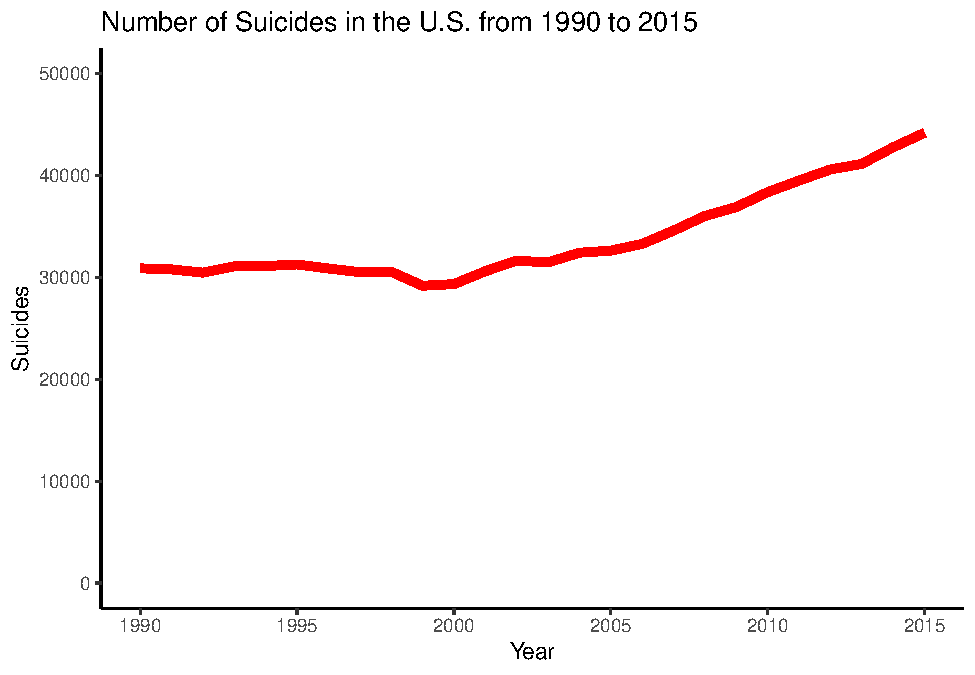
\includegraphics{An-Analysis-of-Suicide-Data_files/figure-latex/unnamed-chunk-1-1.pdf}
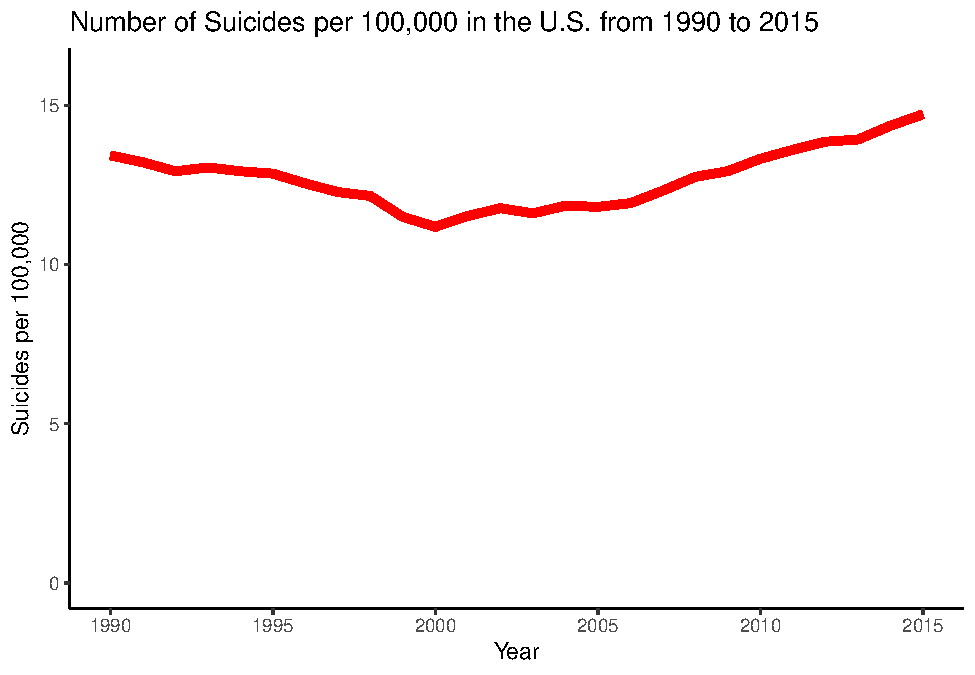
\includegraphics{An-Analysis-of-Suicide-Data_files/figure-latex/unnamed-chunk-1-2.pdf}

\begin{verbatim}
## [1] 43.02962
\end{verbatim}

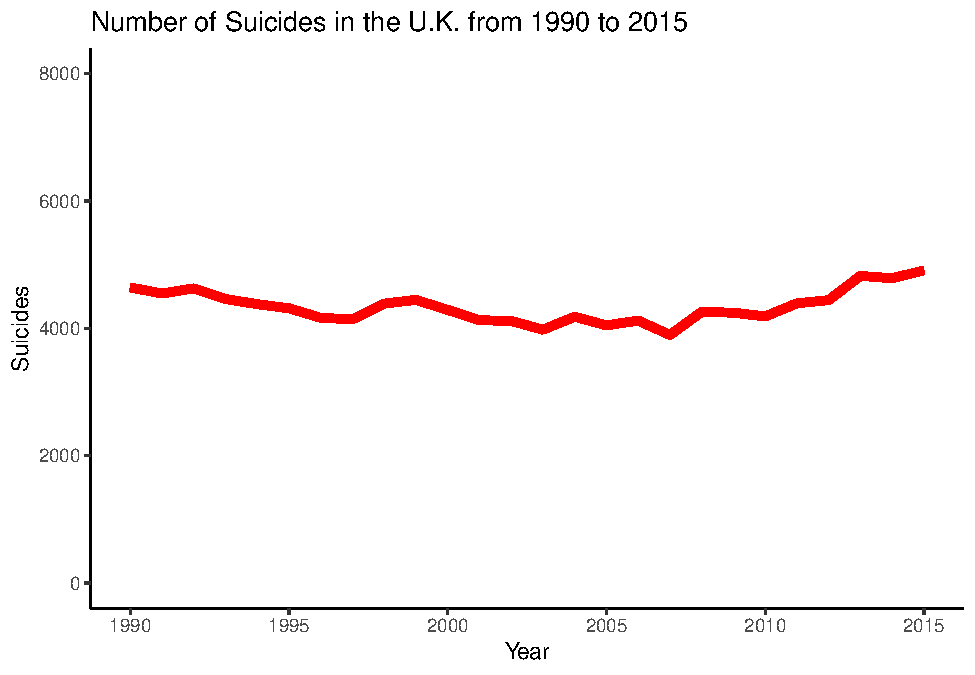
\includegraphics{An-Analysis-of-Suicide-Data_files/figure-latex/unnamed-chunk-1-3.pdf}
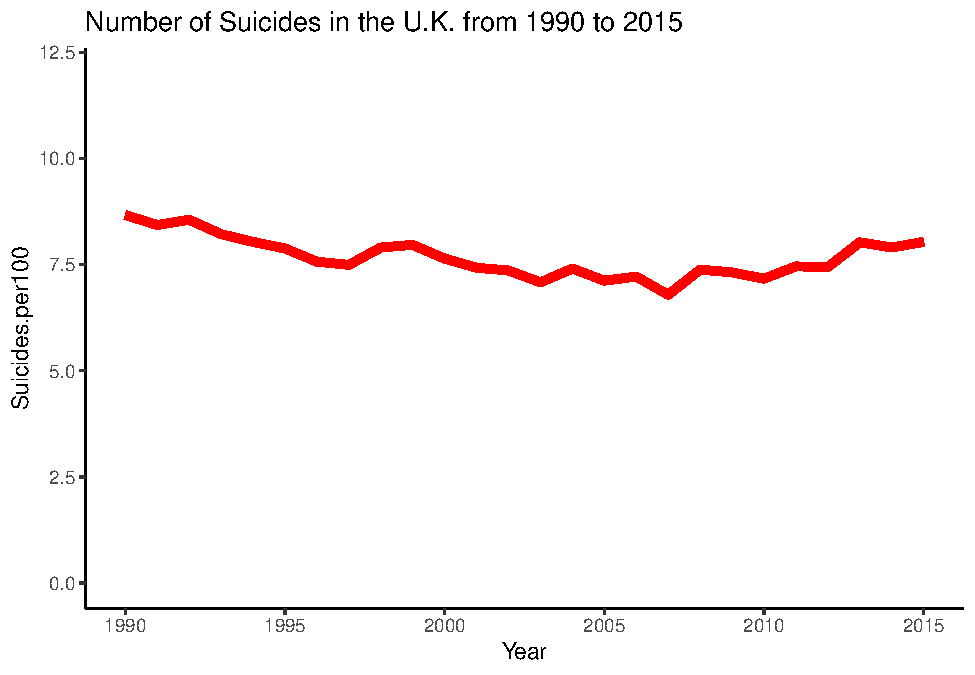
\includegraphics{An-Analysis-of-Suicide-Data_files/figure-latex/unnamed-chunk-1-4.pdf}

\begin{verbatim}
## [1] 11.93042
\end{verbatim}

\begin{verbatim}
## `stat_bin()` using `bins = 30`. Pick better value with `binwidth`.
\end{verbatim}

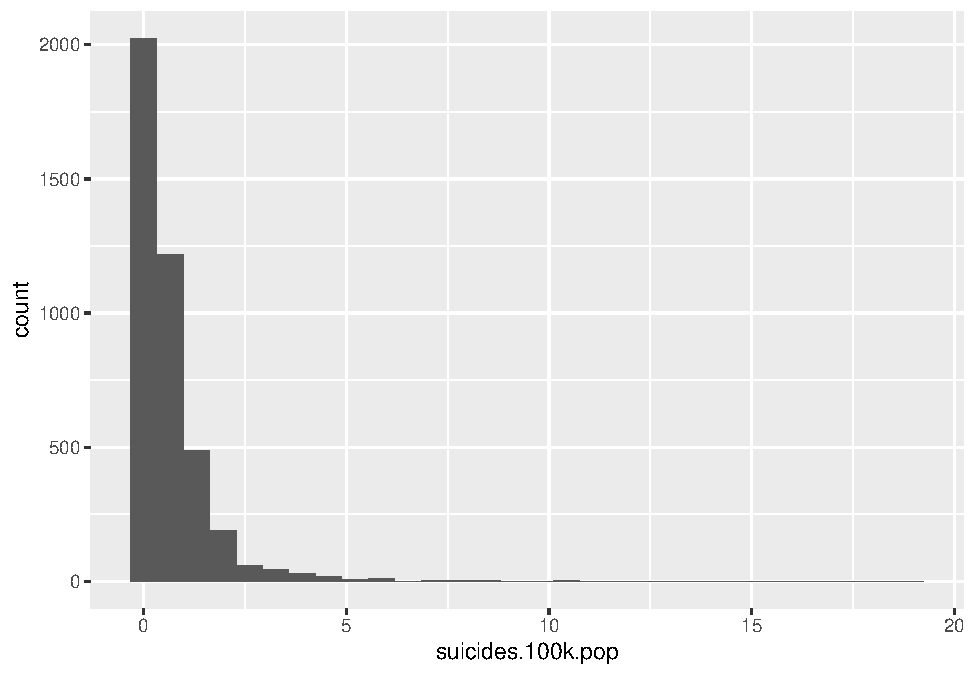
\includegraphics{An-Analysis-of-Suicide-Data_files/figure-latex/unnamed-chunk-1-5.pdf}

\begin{verbatim}
## `stat_bin()` using `bins = 30`. Pick better value with `binwidth`.
\end{verbatim}

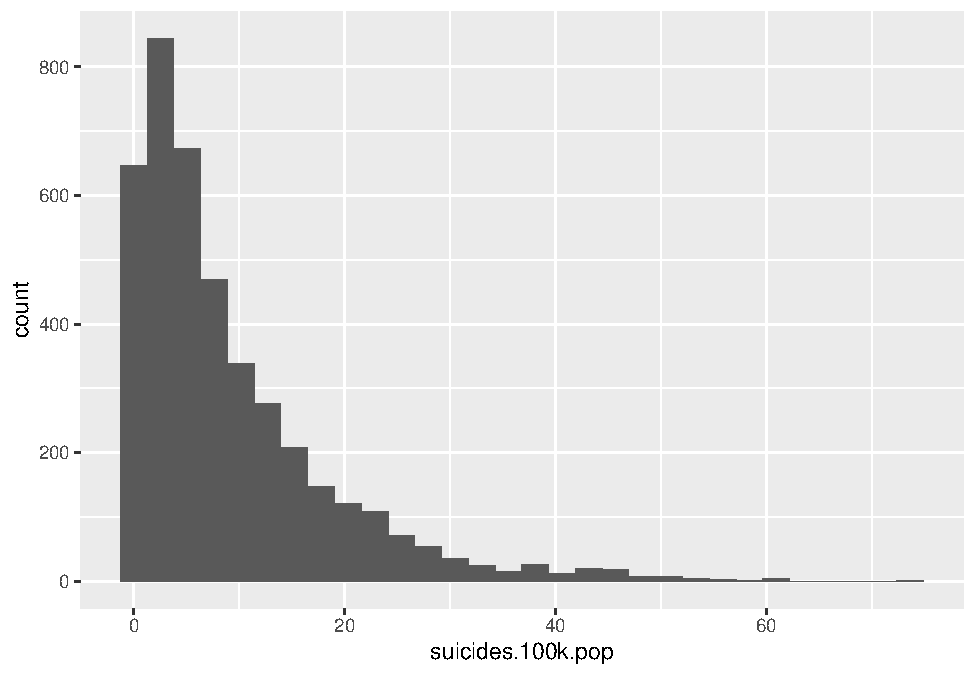
\includegraphics{An-Analysis-of-Suicide-Data_files/figure-latex/unnamed-chunk-1-6.pdf}

\begin{verbatim}
## `stat_bin()` using `bins = 30`. Pick better value with `binwidth`.
\end{verbatim}

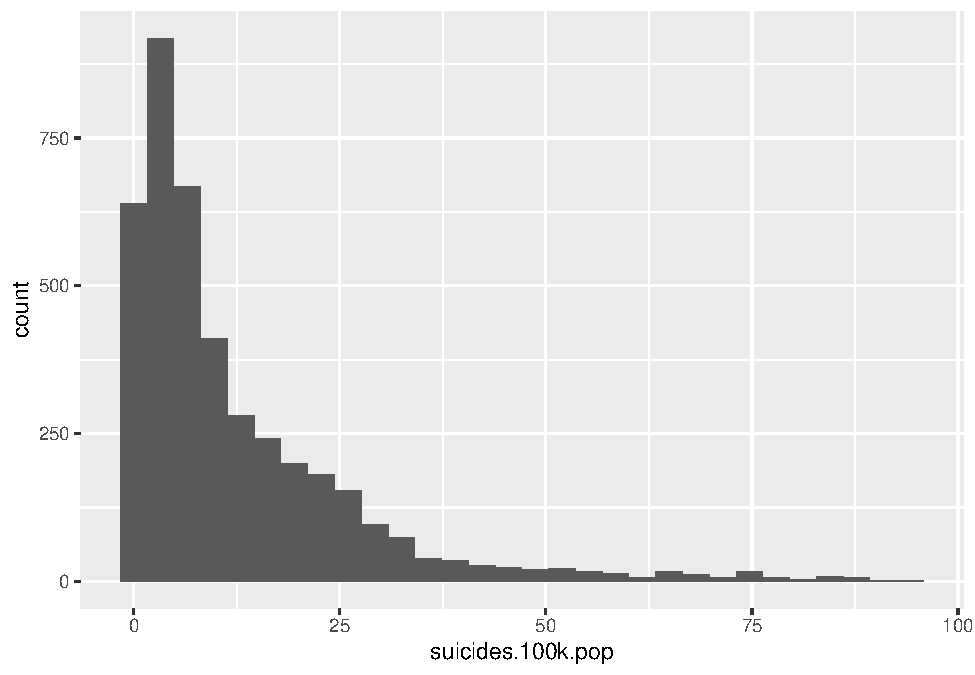
\includegraphics{An-Analysis-of-Suicide-Data_files/figure-latex/unnamed-chunk-1-7.pdf}

\begin{verbatim}
## `stat_bin()` using `bins = 30`. Pick better value with `binwidth`.
\end{verbatim}

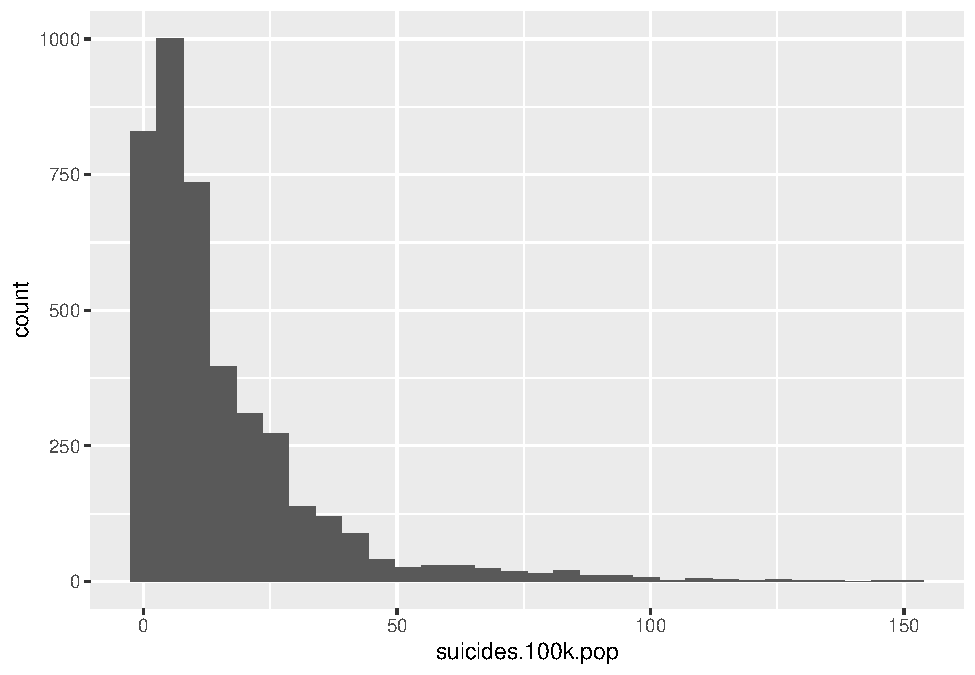
\includegraphics{An-Analysis-of-Suicide-Data_files/figure-latex/unnamed-chunk-1-8.pdf}

\begin{verbatim}
## `stat_bin()` using `bins = 30`. Pick better value with `binwidth`.
\end{verbatim}

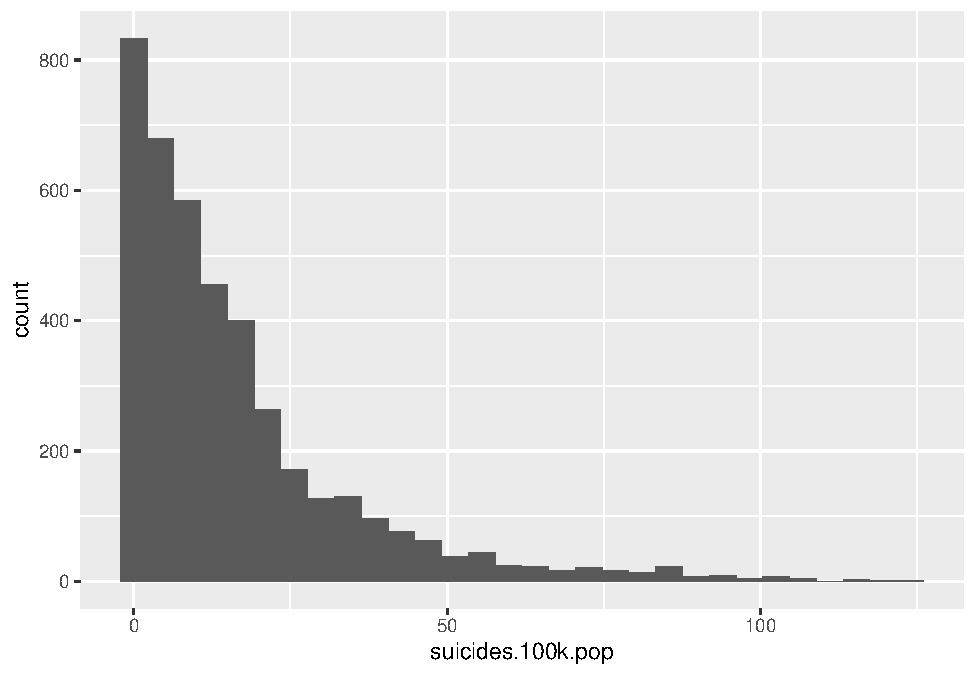
\includegraphics{An-Analysis-of-Suicide-Data_files/figure-latex/unnamed-chunk-1-9.pdf}

\begin{verbatim}
## `stat_bin()` using `bins = 30`. Pick better value with `binwidth`.
\end{verbatim}

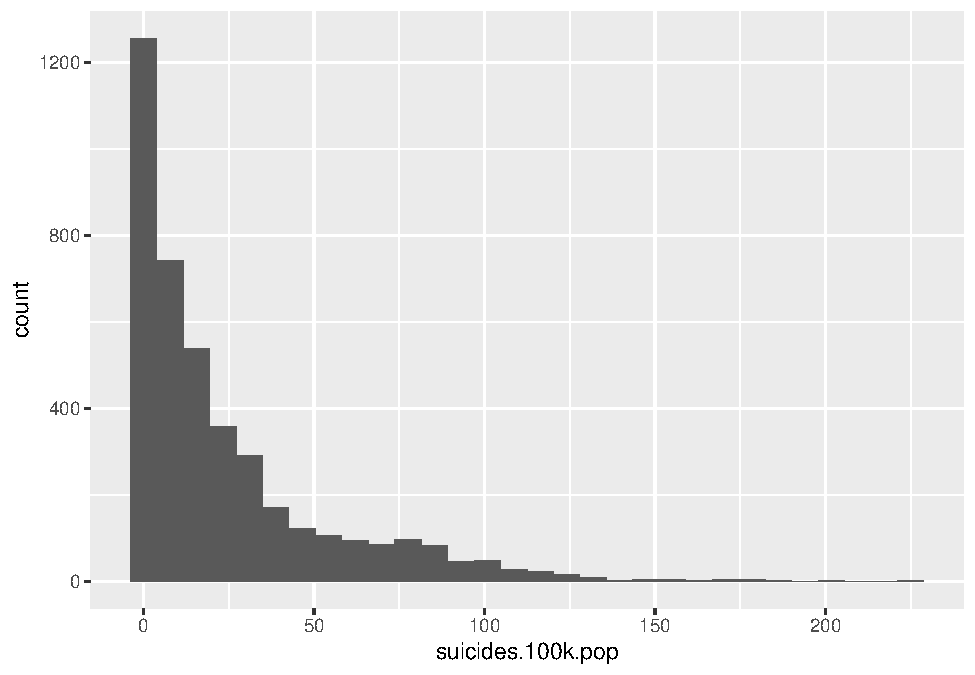
\includegraphics{An-Analysis-of-Suicide-Data_files/figure-latex/unnamed-chunk-1-10.pdf}

\begin{verbatim}
## `stat_bin()` using `bins = 30`. Pick better value with `binwidth`.
\end{verbatim}

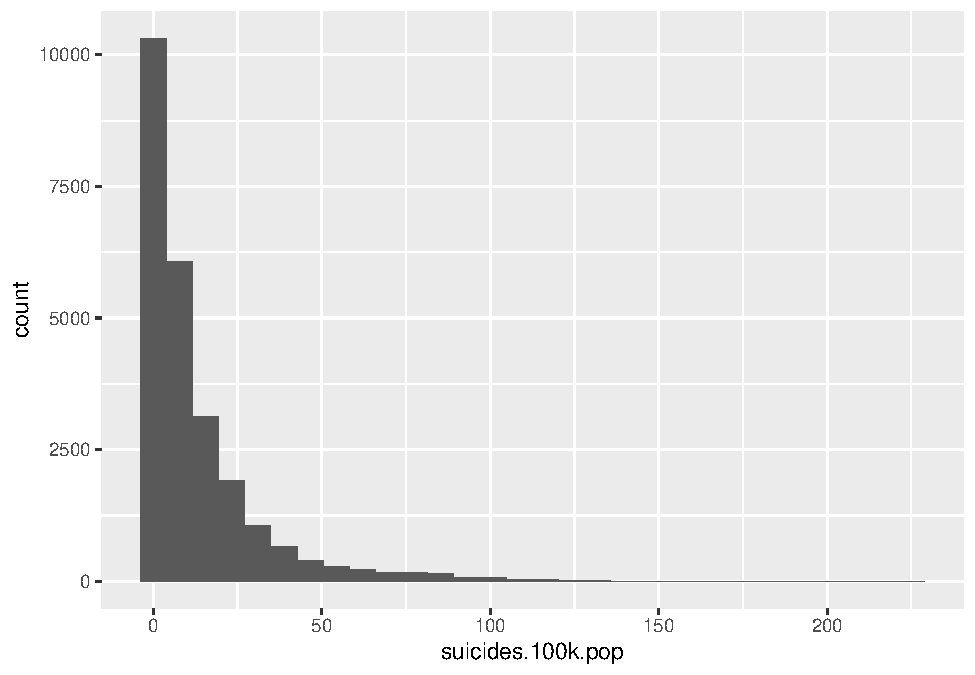
\includegraphics{An-Analysis-of-Suicide-Data_files/figure-latex/unnamed-chunk-1-11.pdf}

\begin{verbatim}
## `stat_bin()` using `bins = 30`. Pick better value with `binwidth`.
\end{verbatim}

\begin{verbatim}
## Warning: Removed 1428 rows containing non-finite values (stat_bin).
\end{verbatim}

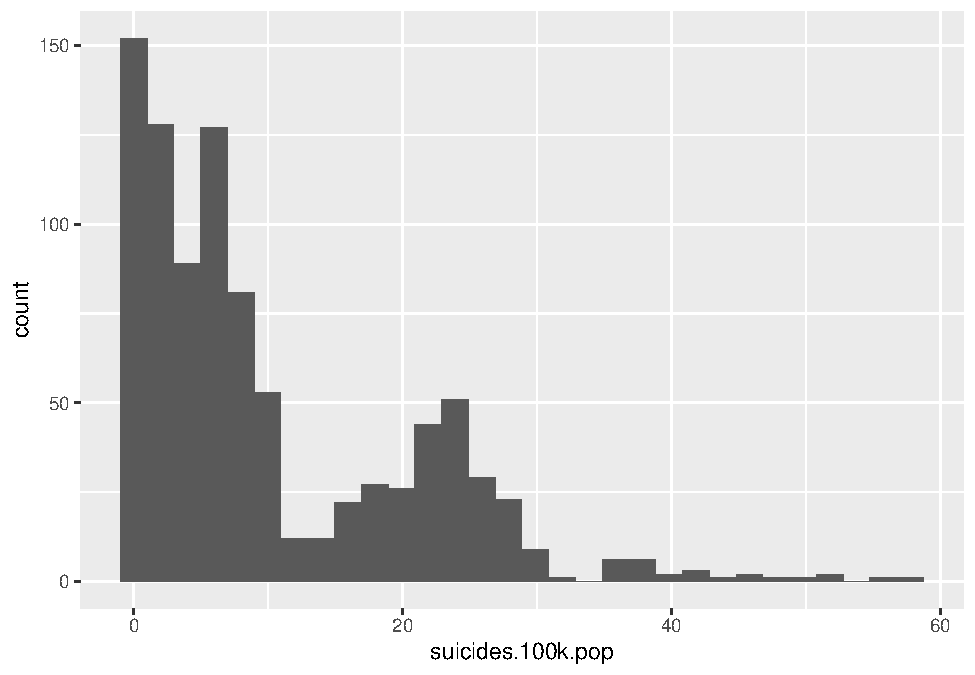
\includegraphics{An-Analysis-of-Suicide-Data_files/figure-latex/unnamed-chunk-1-12.pdf}

\begin{longtable}[]{@{}lr@{}}
\toprule
Region & Mean.suicides\tabularnewline
\midrule
\endhead
Africa & 7.040662\tabularnewline
Asia & 6.142767\tabularnewline
Caribbean & 8.757862\tabularnewline
Central America & 5.888250\tabularnewline
Europe & 16.410372\tabularnewline
North America & 9.804194\tabularnewline
Oceania & 10.988517\tabularnewline
South America & 10.160387\tabularnewline
\bottomrule
\end{longtable}

\hypertarget{demographic-data-model-selection}{%
\section{Demographic Data Model
Selection}\label{demographic-data-model-selection}}

\begin{Shaded}
\begin{Highlighting}[]
\KeywordTok{ls}\NormalTok{(demographic.suicides)}
\end{Highlighting}
\end{Shaded}

\begin{verbatim}
##  [1] "age"               "country"           "Development"      
##  [4] "gdp_for_year"      "gdp_per_capita"    "generation"       
##  [7] "HDI.for.year"      "population"        "Region"           
## [10] "sex"               "suicides.100k.pop" "suicides_no"      
## [13] "year"
\end{verbatim}

\begin{Shaded}
\begin{Highlighting}[]
\CommentTok{## Demographic Model with all relevant predictors (no transformations)}
\NormalTok{demo.fit.all1 <-}\StringTok{ }\KeywordTok{lm}\NormalTok{(suicides}\FloatTok{.100}\NormalTok{k.pop  }\OperatorTok{~}\StringTok{ }\NormalTok{Region }\OperatorTok{+}\StringTok{ }\NormalTok{Development }\OperatorTok{+}\StringTok{ }\NormalTok{age }\OperatorTok{+}\StringTok{ }\NormalTok{gdp_per_capita }\OperatorTok{+}\StringTok{ }\NormalTok{population }\OperatorTok{+}\StringTok{ }\NormalTok{sex }\OperatorTok{+}\StringTok{ }\NormalTok{year, }\DataTypeTok{data =}\NormalTok{ demographic.suicides)}

\CommentTok{# the model has a significant p-value and R^2 of .3605.... most variable are significant.... but first we should check the normality and constant variance assumptions}
\KeywordTok{summary}\NormalTok{(demo.fit.all1)}
\end{Highlighting}
\end{Shaded}

\begin{verbatim}
## 
## Call:
## lm(formula = suicides.100k.pop ~ Region + Development + age + 
##     gdp_per_capita + population + sex + year, data = demographic.suicides)
## 
## Residuals:
##     Min      1Q  Median      3Q     Max 
## -38.159  -8.143  -1.855   4.686 199.328 
## 
## Coefficients:
##                              Estimate Std. Error t value Pr(>|t|)    
## (Intercept)                 2.294e+02  3.009e+01   7.625 2.54e-14 ***
## RegionAsia                  3.060e+00  5.887e-01   5.197 2.04e-07 ***
## RegionCaribbean             1.559e-01  6.184e-01   0.252    0.801    
## RegionCentral America      -7.371e-01  6.631e-01  -1.112    0.266    
## RegionEurope                1.108e+01  5.757e-01  19.244  < 2e-16 ***
## RegionNorth America         3.861e+00  7.961e-01   4.850 1.24e-06 ***
## RegionOceania               4.507e+00  7.508e-01   6.003 1.96e-09 ***
## RegionSouth America         4.231e+00  6.146e-01   6.884 5.97e-12 ***
## Developmentlow or very low -1.478e+00  1.206e+00  -1.225    0.221    
## Developmentmedium          -5.147e-01  3.918e-01  -1.313    0.189    
## Developmentunknown         -4.088e-01  3.164e-01  -1.292    0.196    
## age25-34 years              3.087e+00  3.334e-01   9.259  < 2e-16 ***
## age35-54 years              5.940e+00  3.354e-01  17.713  < 2e-16 ***
## age5-14 years              -8.328e+00  3.341e-01 -24.928  < 2e-16 ***
## age55-74 years              6.992e+00  3.334e-01  20.973  < 2e-16 ***
## age75+ years                1.423e+01  3.353e-01  42.430  < 2e-16 ***
## gdp_per_capita             -7.036e-05  6.111e-06 -11.514  < 2e-16 ***
## population                  1.534e-08  3.031e-08   0.506    0.613    
## sexmale                     1.481e+01  1.926e-01  76.902  < 2e-16 ***
## year                       -1.160e-01  1.499e-02  -7.736 1.07e-14 ***
## ---
## Signif. codes:  0 '***' 0.001 '**' 0.01 '*' 0.05 '.' 0.1 ' ' 1
## 
## Residual standard error: 14.73 on 23360 degrees of freedom
##   (1428 observations deleted due to missingness)
## Multiple R-squared:  0.3605, Adjusted R-squared:   0.36 
## F-statistic: 693.1 on 19 and 23360 DF,  p-value: < 2.2e-16
\end{verbatim}

\begin{Shaded}
\begin{Highlighting}[]
\CommentTok{# there is heteroskedasticity and the residuals are not normally distributed.... we should not use the p-values from the summary above}
\KeywordTok{plot}\NormalTok{(demo.fit.all1, }\DecValTok{1}\NormalTok{)}
\end{Highlighting}
\end{Shaded}

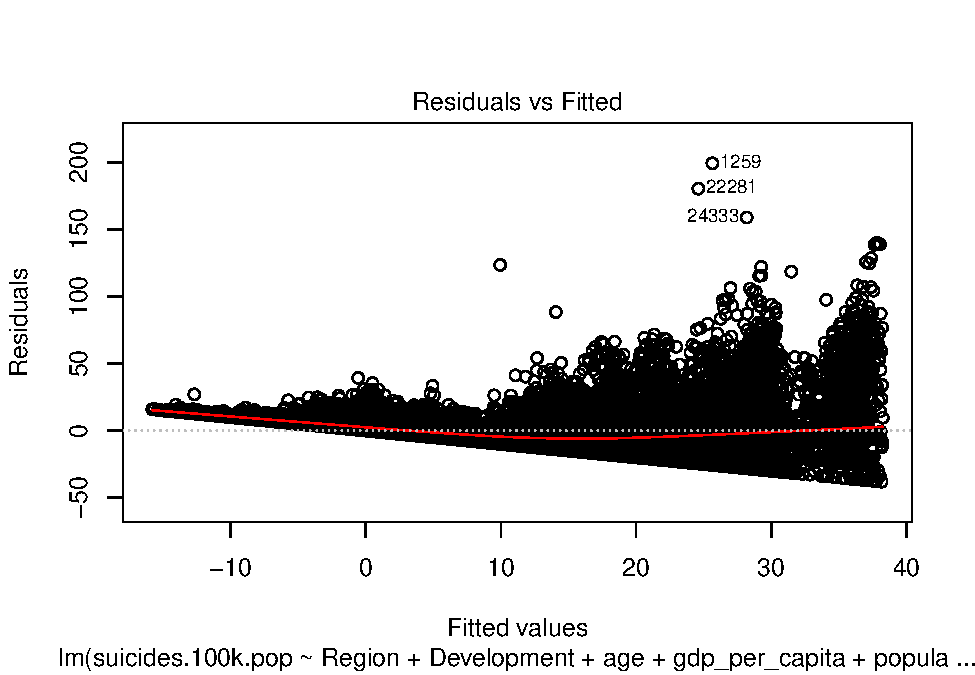
\includegraphics{An-Analysis-of-Suicide-Data_files/figure-latex/unnamed-chunk-2-1.pdf}

\begin{Shaded}
\begin{Highlighting}[]
\KeywordTok{plot}\NormalTok{(demo.fit.all1, }\DecValTok{2}\NormalTok{)}
\end{Highlighting}
\end{Shaded}

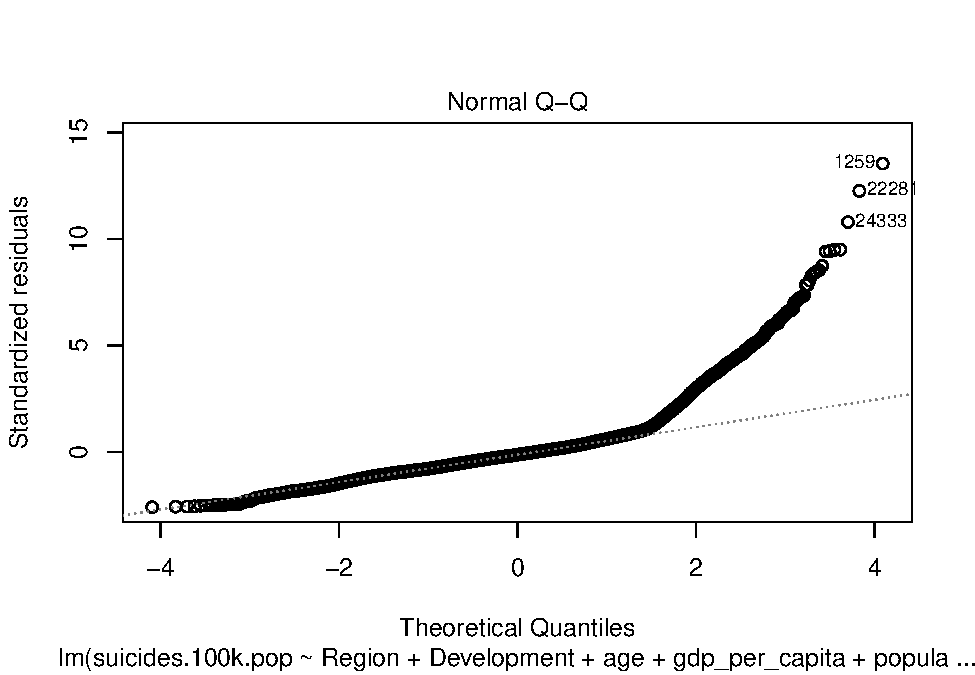
\includegraphics{An-Analysis-of-Suicide-Data_files/figure-latex/unnamed-chunk-2-2.pdf}

\begin{Shaded}
\begin{Highlighting}[]
\CommentTok{## Demographic Model with log(y + 1) transformation}
\CommentTok{# log transformation might get rid of heteroskedasticity (log(X + 1) because some observations have 0 suicides)}
\NormalTok{demo.fit.all2 <-}\StringTok{ }\KeywordTok{lm}\NormalTok{(}\KeywordTok{log}\NormalTok{(suicides}\FloatTok{.100}\NormalTok{k.pop }\OperatorTok{+}\StringTok{ }\DecValTok{1}\NormalTok{) }\OperatorTok{~}\StringTok{ }\NormalTok{Region }\OperatorTok{+}\StringTok{ }\NormalTok{Development }\OperatorTok{+}\StringTok{ }\NormalTok{age }\OperatorTok{+}\StringTok{ }\NormalTok{gdp_per_capita }\OperatorTok{+}\StringTok{ }\NormalTok{population }\OperatorTok{+}\StringTok{ }\NormalTok{sex }\OperatorTok{+}\StringTok{ }\NormalTok{year, }\DataTypeTok{data =}\NormalTok{ demographic.suicides)}

\CommentTok{# R^2 of 0.5271 and a very small p-value... let's check our assumptions}
\KeywordTok{summary}\NormalTok{(demo.fit.all2)}
\end{Highlighting}
\end{Shaded}

\begin{verbatim}
## 
## Call:
## lm(formula = log(suicides.100k.pop + 1) ~ Region + Development + 
##     age + gdp_per_capita + population + sex + year, data = demographic.suicides)
## 
## Residuals:
##     Min      1Q  Median      3Q     Max 
## -3.3400 -0.5408  0.0501  0.5731  3.8513 
## 
## Coefficients:
##                              Estimate Std. Error t value Pr(>|t|)    
## (Intercept)                 1.771e+01  1.801e+00   9.833  < 2e-16 ***
## RegionAsia                  3.703e-01  3.524e-02  10.509  < 2e-16 ***
## RegionCaribbean            -2.440e-01  3.702e-02  -6.593 4.40e-11 ***
## RegionCentral America       1.931e-01  3.969e-02   4.866 1.15e-06 ***
## RegionEurope                9.160e-01  3.446e-02  26.581  < 2e-16 ***
## RegionNorth America         5.439e-01  4.765e-02  11.414  < 2e-16 ***
## RegionOceania               5.751e-01  4.494e-02  12.796  < 2e-16 ***
## RegionSouth America         6.438e-01  3.679e-02  17.502  < 2e-16 ***
## Developmentlow or very low -7.734e-03  7.221e-02  -0.107   0.9147    
## Developmentmedium          -5.496e-02  2.346e-02  -2.343   0.0191 *  
## Developmentunknown         -4.308e-02  1.894e-02  -2.275   0.0229 *  
## age25-34 years              1.870e-01  1.996e-02   9.370  < 2e-16 ***
## age35-54 years              3.535e-01  2.007e-02  17.609  < 2e-16 ***
## age5-14 years              -1.487e+00  2.000e-02 -74.341  < 2e-16 ***
## age55-74 years              3.836e-01  1.996e-02  19.222  < 2e-16 ***
## age75+ years                4.819e-01  2.007e-02  24.005  < 2e-16 ***
## gdp_per_capita             -6.629e-07  3.658e-07  -1.812   0.0699 .  
## population                  1.000e-08  1.814e-09   5.515 3.52e-08 ***
## sexmale                     1.006e+00  1.153e-02  87.268  < 2e-16 ***
## year                       -8.422e-03  8.973e-04  -9.386  < 2e-16 ***
## ---
## Signif. codes:  0 '***' 0.001 '**' 0.01 '*' 0.05 '.' 0.1 ' ' 1
## 
## Residual standard error: 0.8815 on 23360 degrees of freedom
##   (1428 observations deleted due to missingness)
## Multiple R-squared:  0.5271, Adjusted R-squared:  0.5268 
## F-statistic:  1371 on 19 and 23360 DF,  p-value: < 2.2e-16
\end{verbatim}

\begin{Shaded}
\begin{Highlighting}[]
\CommentTok{# both of our assumptions are roughly met (normality more-so)... considering the shape of the residual variance we should be cautious with inference}
\CommentTok{# perhaps a zero-infalted model would be better but we can still gain some insightful information from our model}
\KeywordTok{plot}\NormalTok{(demo.fit.all2, }\DecValTok{1}\NormalTok{)}
\end{Highlighting}
\end{Shaded}

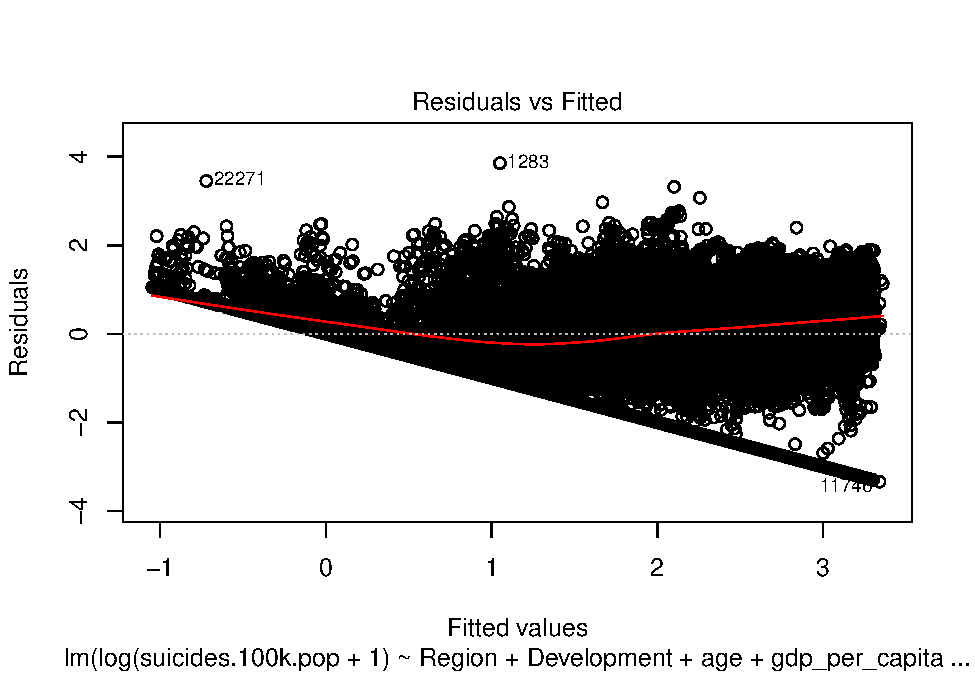
\includegraphics{An-Analysis-of-Suicide-Data_files/figure-latex/unnamed-chunk-2-3.pdf}

\begin{Shaded}
\begin{Highlighting}[]
\KeywordTok{plot}\NormalTok{(demo.fit.all2, }\DecValTok{2}\NormalTok{)}
\end{Highlighting}
\end{Shaded}

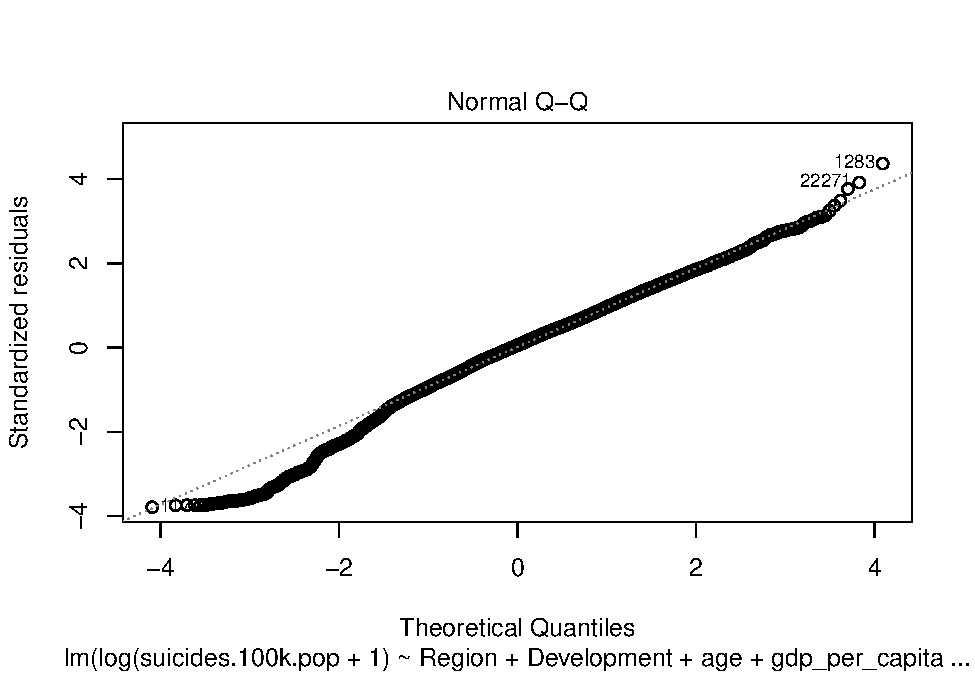
\includegraphics{An-Analysis-of-Suicide-Data_files/figure-latex/unnamed-chunk-2-4.pdf}

\begin{Shaded}
\begin{Highlighting}[]
\CommentTok{## Demographic Model with log(y) transformation and observations with 0 suicides are removed}
\NormalTok{demo.fit.all3 <-}\StringTok{ }\KeywordTok{lm}\NormalTok{(}\KeywordTok{log}\NormalTok{(suicides}\FloatTok{.100}\NormalTok{k.pop) }\OperatorTok{~}\StringTok{ }\NormalTok{Region }\OperatorTok{+}\StringTok{ }\NormalTok{Development }\OperatorTok{+}\StringTok{ }\NormalTok{age }\OperatorTok{+}\StringTok{ }\NormalTok{gdp_per_capita }\OperatorTok{+}\StringTok{ }\NormalTok{population }\OperatorTok{+}\StringTok{ }\NormalTok{sex }\OperatorTok{+}\StringTok{ }\NormalTok{year, }\DataTypeTok{data =}\NormalTok{ demo.subset.rm)}

\CommentTok{# R^2 of .6568 and and very significant p-value... let's look at residual diagnostics}
\KeywordTok{summary}\NormalTok{(demo.fit.all3)}
\end{Highlighting}
\end{Shaded}

\begin{verbatim}
## 
## Call:
## lm(formula = log(suicides.100k.pop) ~ Region + Development + 
##     age + gdp_per_capita + population + sex + year, data = demo.subset.rm)
## 
## Residuals:
##     Min      1Q  Median      3Q     Max 
## -4.2215 -0.5107  0.0621  0.5669  4.6899 
## 
## Coefficients:
##                              Estimate Std. Error  t value Pr(>|t|)    
## (Intercept)                 1.898e+01  1.887e+00   10.055  < 2e-16 ***
## RegionAsia                  5.421e-01  3.899e-02   13.902  < 2e-16 ***
## RegionCaribbean             7.794e-01  4.433e-02   17.582  < 2e-16 ***
## RegionCentral America       3.641e-01  4.372e-02    8.328  < 2e-16 ***
## RegionEurope                1.061e+00  3.817e-02   27.784  < 2e-16 ***
## RegionNorth America         7.113e-01  4.972e-02   14.305  < 2e-16 ***
## RegionOceania               9.868e-01  4.940e-02   19.976  < 2e-16 ***
## RegionSouth America         7.736e-01  4.009e-02   19.297  < 2e-16 ***
## Developmentlow or very low -1.261e-01  7.263e-02   -1.736  0.08255 .  
## Developmentmedium          -3.805e-02  2.454e-02   -1.551  0.12102    
## Developmentunknown         -1.670e-02  1.946e-02   -0.858  0.39065    
## age25-34 years              2.061e-01  2.053e-02   10.041  < 2e-16 ***
## age35-54 years              3.710e-01  2.055e-02   18.058  < 2e-16 ***
## age5-14 years              -2.449e+00  2.213e-02 -110.638  < 2e-16 ***
## age55-74 years              4.793e-01  2.060e-02   23.264  < 2e-16 ***
## age75+ years                8.239e-01  2.123e-02   38.800  < 2e-16 ***
## gdp_per_capita             -2.193e-07  3.866e-07   -0.567  0.57060    
## population                 -5.425e-09  1.793e-09   -3.025  0.00249 ** 
## sexmale                     1.201e+00  1.220e-02   98.430  < 2e-16 ***
## year                       -9.234e-03  9.402e-04   -9.821  < 2e-16 ***
## ---
## Signif. codes:  0 '***' 0.001 '**' 0.01 '*' 0.05 '.' 0.1 ' ' 1
## 
## Residual standard error: 0.8609 on 19978 degrees of freedom
##   (1079 observations deleted due to missingness)
## Multiple R-squared:  0.6568, Adjusted R-squared:  0.6565 
## F-statistic:  2013 on 19 and 19978 DF,  p-value: < 2.2e-16
\end{verbatim}

\begin{Shaded}
\begin{Highlighting}[]
\CommentTok{# q-q plot is fine... not perfect but good enough considering our sample size. Residuals vs. fitted is much better than the model of log(y+1)...}
\CommentTok{# likely because zeros were removed}
\KeywordTok{plot}\NormalTok{(demo.fit.all3, }\DecValTok{1}\NormalTok{)}
\end{Highlighting}
\end{Shaded}

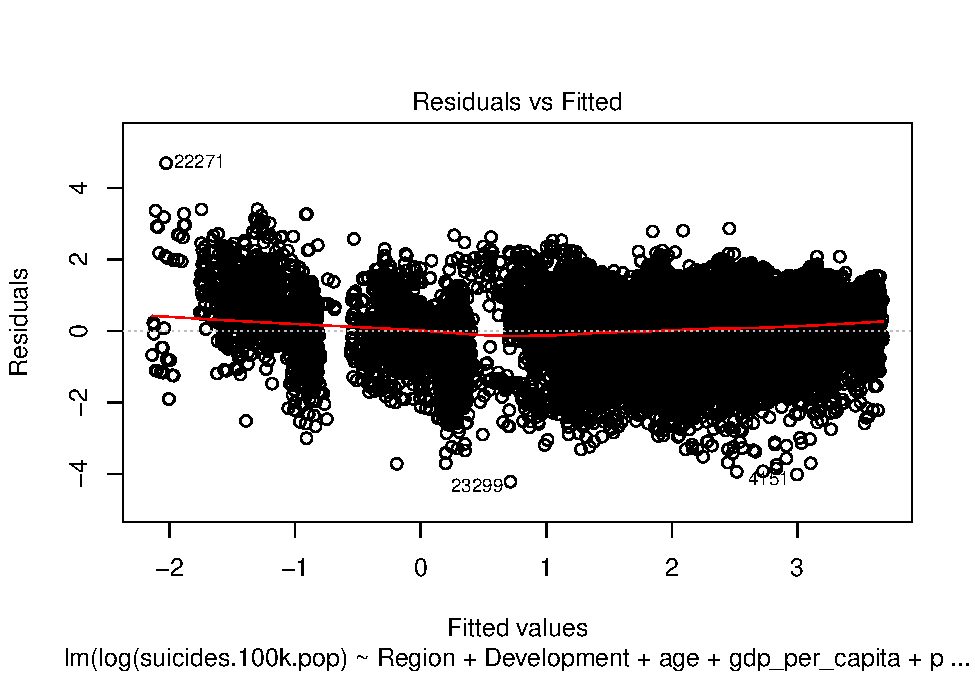
\includegraphics{An-Analysis-of-Suicide-Data_files/figure-latex/unnamed-chunk-2-5.pdf}

\begin{Shaded}
\begin{Highlighting}[]
\KeywordTok{plot}\NormalTok{(demo.fit.all3, }\DecValTok{2}\NormalTok{)}
\end{Highlighting}
\end{Shaded}

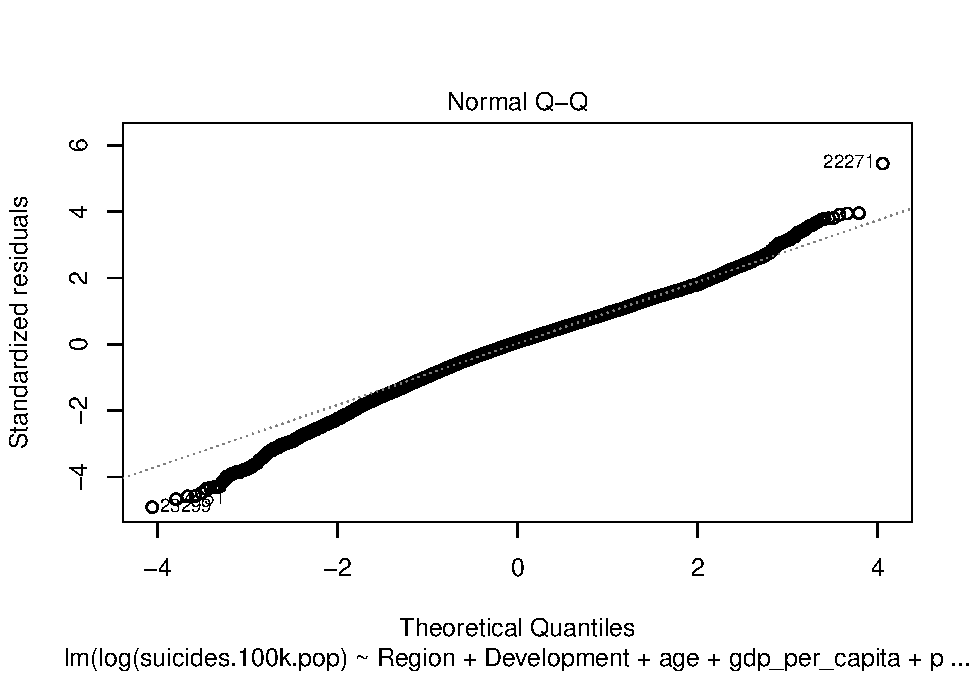
\includegraphics{An-Analysis-of-Suicide-Data_files/figure-latex/unnamed-chunk-2-6.pdf}

\begin{Shaded}
\begin{Highlighting}[]
\CommentTok{## before choosing a model, we should look at the practicality of the models for predicting... especially since log(y+1) is modeling a different response}

\CommentTok{# prediction plot for log + 1}
\NormalTok{mean.pop <-}\StringTok{ }\KeywordTok{mean}\NormalTok{(aggregate.suicides[aggregate.suicides}\OperatorTok{$}\NormalTok{Region }\OperatorTok{==}\StringTok{ "North America"} \OperatorTok{&}\StringTok{ }\NormalTok{aggregate.suicides}\OperatorTok{$}\NormalTok{Year }\OperatorTok{==}\StringTok{ }\DecValTok{2015}\NormalTok{,]}\OperatorTok{$}\NormalTok{Population, }\DataTypeTok{na.rm =} \OtherTok{TRUE}\NormalTok{)}
\NormalTok{year.pred <-}\StringTok{ }\DecValTok{2015}
\NormalTok{age.pred <-}\StringTok{ "25-34 years"}
\NormalTok{region.pred <-}\StringTok{ "North America"}
\NormalTok{develop.pred <-}\StringTok{ "high"}
\NormalTok{gdp.seq <-}\StringTok{ }\KeywordTok{seq}\NormalTok{(}\KeywordTok{min}\NormalTok{(aggregate.suicides}\OperatorTok{$}\NormalTok{GDP.per.capita), }\KeywordTok{max}\NormalTok{(aggregate.suicides}\OperatorTok{$}\NormalTok{GDP.per.capita), }\DataTypeTok{length.out =} \DecValTok{1000}\NormalTok{)}
\NormalTok{sex.pred <-}\StringTok{ }\KeywordTok{c}\NormalTok{(}\StringTok{"male"}\NormalTok{, }\StringTok{"female"}\NormalTok{)}

\NormalTok{expand.grid.demo <-}\StringTok{ }\KeywordTok{expand.grid}\NormalTok{(region.pred, develop.pred, age.pred, gdp.seq, mean.pop, sex.pred, year.pred)}
\KeywordTok{colnames}\NormalTok{(expand.grid.demo) <-}\StringTok{ }\KeywordTok{c}\NormalTok{(}\StringTok{"Region"}\NormalTok{, }\StringTok{"Development"}\NormalTok{, }\StringTok{"age"}\NormalTok{, }\StringTok{"gdp_per_capita"}\NormalTok{, }\StringTok{"population"}\NormalTok{, }\StringTok{"sex"}\NormalTok{, }\StringTok{"year"}\NormalTok{)}

\NormalTok{demo.expand.pred <-}\StringTok{ }\KeywordTok{predict}\NormalTok{(demo.fit.all2, }\DataTypeTok{newdata =}\NormalTok{ expand.grid.demo)}

\NormalTok{demo.pred.data <-}\StringTok{ }\KeywordTok{cbind}\NormalTok{(expand.grid.demo, demo.expand.pred)}
\KeywordTok{colnames}\NormalTok{(demo.pred.data) <-}\StringTok{ }\KeywordTok{c}\NormalTok{(}\StringTok{"Region"}\NormalTok{, }\StringTok{"Development"}\NormalTok{, }\StringTok{"age"}\NormalTok{, }\StringTok{"gdp_per_capita"}\NormalTok{, }\StringTok{"population"}\NormalTok{, }\StringTok{"sex"}\NormalTok{, }\StringTok{"year"}\NormalTok{, }\StringTok{"suicides.100k.pop"}\NormalTok{)}

\KeywordTok{ggplot}\NormalTok{(demo.pred.data, }\KeywordTok{aes}\NormalTok{(}\DataTypeTok{x =}\NormalTok{ gdp_per_capita, }\DataTypeTok{y =} \KeywordTok{exp}\NormalTok{(suicides}\FloatTok{.100}\NormalTok{k.pop)}\OperatorTok{-}\DecValTok{1}\NormalTok{, }\DataTypeTok{color =}\NormalTok{ sex)) }\OperatorTok{+}\StringTok{ }
\StringTok{  }\KeywordTok{geom_line}\NormalTok{() }\OperatorTok{+}\StringTok{ }
\StringTok{  }\KeywordTok{labs}\NormalTok{(}\DataTypeTok{x =} \StringTok{"GDP per capita"}\NormalTok{, }\DataTypeTok{y =} \StringTok{"Predicted Suicides per 100k"}\NormalTok{, }\DataTypeTok{title =} \StringTok{"Predicted Suicides for Males and Females"}\NormalTok{) }\OperatorTok{+}
\StringTok{  }\KeywordTok{lims}\NormalTok{(}\DataTypeTok{x =} \KeywordTok{c}\NormalTok{(}\DecValTok{0}\NormalTok{, }\DecValTok{10000}\NormalTok{), }\DataTypeTok{y =} \KeywordTok{c}\NormalTok{(}\DecValTok{0}\NormalTok{, }\DecValTok{100}\NormalTok{))}
\end{Highlighting}
\end{Shaded}

\begin{verbatim}
## Warning: Removed 1844 rows containing missing values (geom_path).
\end{verbatim}

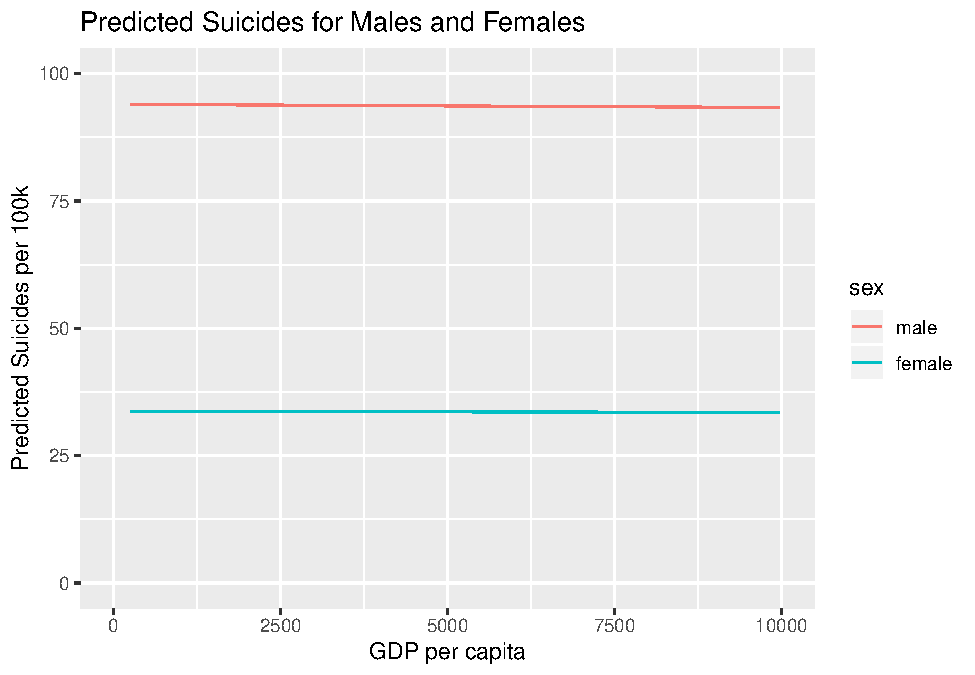
\includegraphics{An-Analysis-of-Suicide-Data_files/figure-latex/unnamed-chunk-2-7.pdf}

\begin{Shaded}
\begin{Highlighting}[]
\CommentTok{# this model is not predicting properly... at all... this is because it is modeling a totally different response log(y +1) not log(y)}
\KeywordTok{mean}\NormalTok{(aggregate.suicides[aggregate.suicides}\OperatorTok{$}\NormalTok{Year }\OperatorTok{==}\StringTok{ }\DecValTok{2015} \OperatorTok{&}\StringTok{ }\NormalTok{aggregate.suicides}\OperatorTok{$}\NormalTok{Region }\OperatorTok{==}\StringTok{ "North America"}\NormalTok{,]}\OperatorTok{$}\NormalTok{Suicides.per100, }\DataTypeTok{na.rm =} \OtherTok{TRUE}\NormalTok{)}
\end{Highlighting}
\end{Shaded}

\begin{verbatim}
## [1] 10.08856
\end{verbatim}

\begin{Shaded}
\begin{Highlighting}[]
\CommentTok{# plot for removed 0s}
\NormalTok{mean.pop <-}\StringTok{ }\KeywordTok{mean}\NormalTok{(aggregate.suicides[aggregate.suicides}\OperatorTok{$}\NormalTok{Region }\OperatorTok{==}\StringTok{ "North America"} \OperatorTok{&}\StringTok{ }\NormalTok{aggregate.suicides}\OperatorTok{$}\NormalTok{Year }\OperatorTok{==}\StringTok{ }\DecValTok{2015}\NormalTok{,]}\OperatorTok{$}\NormalTok{Population, }\DataTypeTok{na.rm =} \OtherTok{TRUE}\NormalTok{)}
\NormalTok{year.pred <-}\StringTok{ }\DecValTok{2015}
\NormalTok{age.pred <-}\StringTok{ "25-34 years"}
\NormalTok{region.pred <-}\StringTok{ "North America"}
\NormalTok{develop.pred <-}\StringTok{ "high"}
\NormalTok{gdp.seq <-}\StringTok{ }\KeywordTok{seq}\NormalTok{(}\KeywordTok{min}\NormalTok{(aggregate.suicides}\OperatorTok{$}\NormalTok{GDP.per.capita), }\KeywordTok{max}\NormalTok{(aggregate.suicides}\OperatorTok{$}\NormalTok{GDP.per.capita), }\DataTypeTok{length.out =} \DecValTok{1000}\NormalTok{)}
\NormalTok{sex.pred <-}\StringTok{ }\KeywordTok{c}\NormalTok{(}\StringTok{"male"}\NormalTok{, }\StringTok{"female"}\NormalTok{)}

\NormalTok{expand.grid.demo <-}\StringTok{ }\KeywordTok{expand.grid}\NormalTok{(region.pred, develop.pred, age.pred, gdp.seq, mean.pop, sex.pred, year.pred)}
\KeywordTok{colnames}\NormalTok{(expand.grid.demo) <-}\StringTok{ }\KeywordTok{c}\NormalTok{(}\StringTok{"Region"}\NormalTok{, }\StringTok{"Development"}\NormalTok{, }\StringTok{"age"}\NormalTok{, }\StringTok{"gdp_per_capita"}\NormalTok{, }\StringTok{"population"}\NormalTok{, }\StringTok{"sex"}\NormalTok{, }\StringTok{"year"}\NormalTok{)}

\NormalTok{demo.expand.pred <-}\StringTok{ }\KeywordTok{predict}\NormalTok{(demo.fit.all3, }\DataTypeTok{newdata =}\NormalTok{ expand.grid.demo)}

\NormalTok{demo.pred.data <-}\StringTok{ }\KeywordTok{cbind}\NormalTok{(expand.grid.demo, demo.expand.pred)}
\KeywordTok{colnames}\NormalTok{(demo.pred.data) <-}\StringTok{ }\KeywordTok{c}\NormalTok{(}\StringTok{"Region"}\NormalTok{, }\StringTok{"Development"}\NormalTok{, }\StringTok{"age"}\NormalTok{, }\StringTok{"gdp_per_capita"}\NormalTok{, }\StringTok{"population"}\NormalTok{, }\StringTok{"sex"}\NormalTok{, }\StringTok{"year"}\NormalTok{, }\StringTok{"suicides.100k.pop"}\NormalTok{)}

\KeywordTok{ggplot}\NormalTok{(demo.pred.data, }\KeywordTok{aes}\NormalTok{(}\DataTypeTok{x =}\NormalTok{ gdp_per_capita, }\DataTypeTok{y =} \KeywordTok{exp}\NormalTok{(suicides}\FloatTok{.100}\NormalTok{k.pop), }\DataTypeTok{color =}\NormalTok{ sex)) }\OperatorTok{+}\StringTok{ }
\StringTok{  }\KeywordTok{geom_line}\NormalTok{() }\OperatorTok{+}\StringTok{ }
\StringTok{  }\KeywordTok{labs}\NormalTok{(}\DataTypeTok{x =} \StringTok{"GDP per capita"}\NormalTok{, }\DataTypeTok{y =} \StringTok{"Predicted Suicides per 100k"}\NormalTok{, }\DataTypeTok{title =} \StringTok{"Predicted Suicides for Males and Females"}\NormalTok{) }\OperatorTok{+}
\StringTok{  }\KeywordTok{lims}\NormalTok{(}\DataTypeTok{x =} \KeywordTok{c}\NormalTok{(}\DecValTok{0}\NormalTok{, }\DecValTok{100000}\NormalTok{), }\DataTypeTok{y =} \KeywordTok{c}\NormalTok{(}\DecValTok{0}\NormalTok{, }\DecValTok{6}\NormalTok{))}
\end{Highlighting}
\end{Shaded}

\begin{verbatim}
## Warning: Removed 418 rows containing missing values (geom_path).
\end{verbatim}

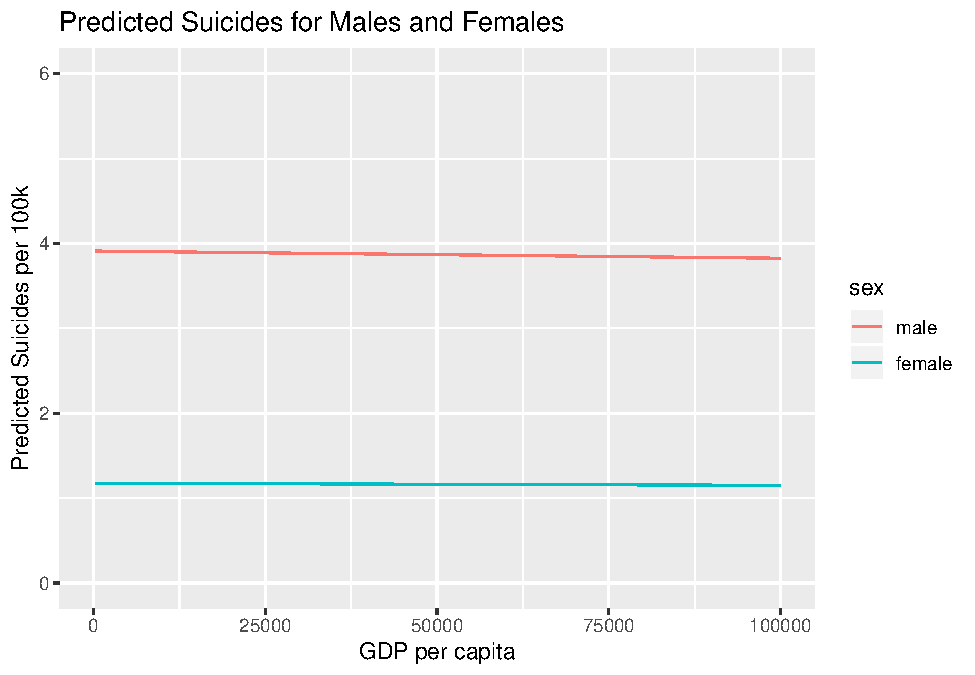
\includegraphics{An-Analysis-of-Suicide-Data_files/figure-latex/unnamed-chunk-2-8.pdf}

\begin{Shaded}
\begin{Highlighting}[]
\CommentTok{# this model does much better at predicting realistic values... although a zero inflated model would be much prefferred.... I'm going with }
\CommentTok{# removing 0s for the rest of the project}
\KeywordTok{mean}\NormalTok{(aggregate.suicides[aggregate.suicides}\OperatorTok{$}\NormalTok{Year }\OperatorTok{==}\StringTok{ }\DecValTok{2015} \OperatorTok{&}\StringTok{ }\NormalTok{aggregate.suicides}\OperatorTok{$}\NormalTok{Region }\OperatorTok{==}\StringTok{ "North America"}\NormalTok{,]}\OperatorTok{$}\NormalTok{Suicides.per100, }\DataTypeTok{na.rm =} \OtherTok{TRUE}\NormalTok{)}
\end{Highlighting}
\end{Shaded}

\begin{verbatim}
## [1] 10.08856
\end{verbatim}

I have decided to remove all the observations with 0 suicides due to the
transformation of log(y + 1) being poor in practical predictions.

\hypertarget{final-model-for-demographic-data}{%
\subsection{Final Model for Demographic
Data}\label{final-model-for-demographic-data}}

\begin{Shaded}
\begin{Highlighting}[]
\CommentTok{# summary output for the final model log(y)}
\KeywordTok{summary}\NormalTok{(demo.fit.all3)}
\end{Highlighting}
\end{Shaded}

\begin{verbatim}
## 
## Call:
## lm(formula = log(suicides.100k.pop) ~ Region + Development + 
##     age + gdp_per_capita + population + sex + year, data = demo.subset.rm)
## 
## Residuals:
##     Min      1Q  Median      3Q     Max 
## -4.2215 -0.5107  0.0621  0.5669  4.6899 
## 
## Coefficients:
##                              Estimate Std. Error  t value Pr(>|t|)    
## (Intercept)                 1.898e+01  1.887e+00   10.055  < 2e-16 ***
## RegionAsia                  5.421e-01  3.899e-02   13.902  < 2e-16 ***
## RegionCaribbean             7.794e-01  4.433e-02   17.582  < 2e-16 ***
## RegionCentral America       3.641e-01  4.372e-02    8.328  < 2e-16 ***
## RegionEurope                1.061e+00  3.817e-02   27.784  < 2e-16 ***
## RegionNorth America         7.113e-01  4.972e-02   14.305  < 2e-16 ***
## RegionOceania               9.868e-01  4.940e-02   19.976  < 2e-16 ***
## RegionSouth America         7.736e-01  4.009e-02   19.297  < 2e-16 ***
## Developmentlow or very low -1.261e-01  7.263e-02   -1.736  0.08255 .  
## Developmentmedium          -3.805e-02  2.454e-02   -1.551  0.12102    
## Developmentunknown         -1.670e-02  1.946e-02   -0.858  0.39065    
## age25-34 years              2.061e-01  2.053e-02   10.041  < 2e-16 ***
## age35-54 years              3.710e-01  2.055e-02   18.058  < 2e-16 ***
## age5-14 years              -2.449e+00  2.213e-02 -110.638  < 2e-16 ***
## age55-74 years              4.793e-01  2.060e-02   23.264  < 2e-16 ***
## age75+ years                8.239e-01  2.123e-02   38.800  < 2e-16 ***
## gdp_per_capita             -2.193e-07  3.866e-07   -0.567  0.57060    
## population                 -5.425e-09  1.793e-09   -3.025  0.00249 ** 
## sexmale                     1.201e+00  1.220e-02   98.430  < 2e-16 ***
## year                       -9.234e-03  9.402e-04   -9.821  < 2e-16 ***
## ---
## Signif. codes:  0 '***' 0.001 '**' 0.01 '*' 0.05 '.' 0.1 ' ' 1
## 
## Residual standard error: 0.8609 on 19978 degrees of freedom
##   (1079 observations deleted due to missingness)
## Multiple R-squared:  0.6568, Adjusted R-squared:  0.6565 
## F-statistic:  2013 on 19 and 19978 DF,  p-value: < 2.2e-16
\end{verbatim}

\begin{Shaded}
\begin{Highlighting}[]
\CommentTok{# residual diagnostics}
\KeywordTok{plot}\NormalTok{(demo.fit.all3, }\DecValTok{1}\NormalTok{)}
\end{Highlighting}
\end{Shaded}

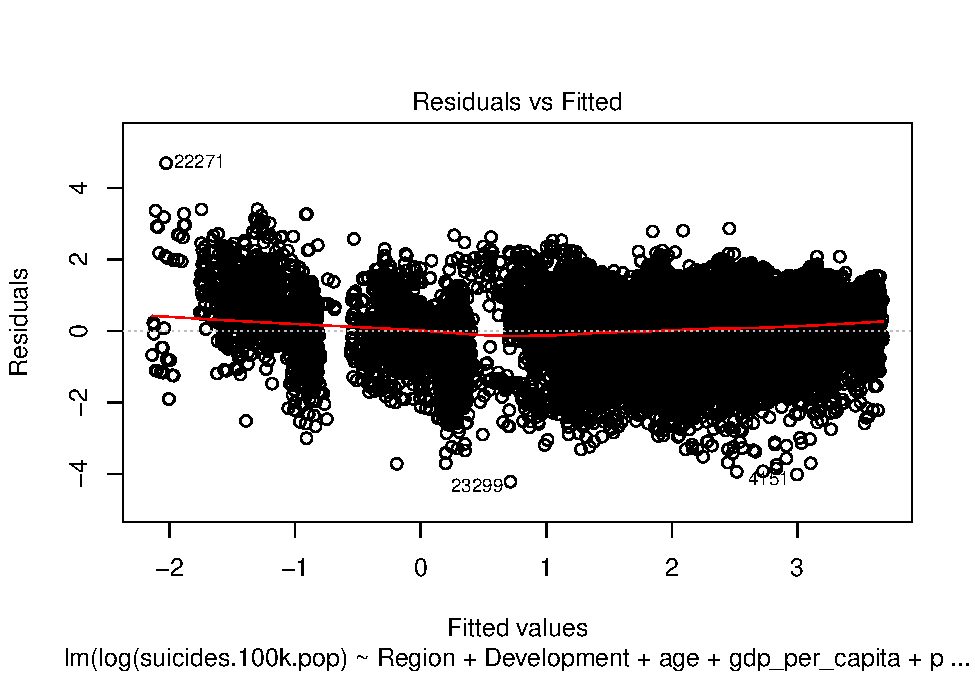
\includegraphics{An-Analysis-of-Suicide-Data_files/figure-latex/unnamed-chunk-3-1.pdf}

\begin{Shaded}
\begin{Highlighting}[]
\KeywordTok{plot}\NormalTok{(demo.fit.all3, }\DecValTok{2}\NormalTok{)}
\end{Highlighting}
\end{Shaded}

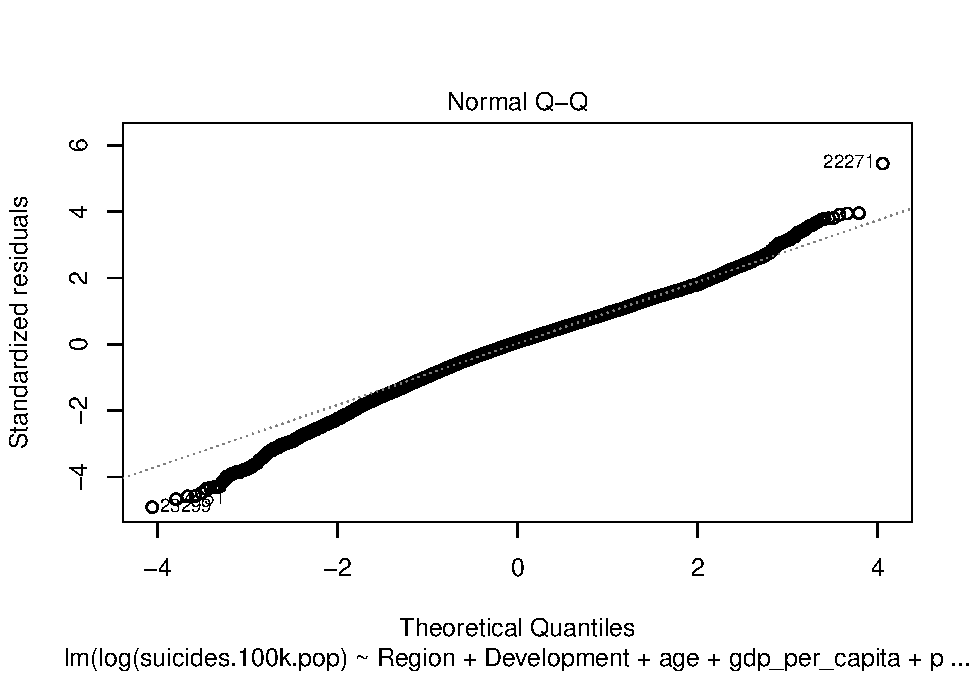
\includegraphics{An-Analysis-of-Suicide-Data_files/figure-latex/unnamed-chunk-3-2.pdf}

\hypertarget{model-interpretation-and-visualization}{%
\subsection{Model Interpretation and
Visualization}\label{model-interpretation-and-visualization}}

\begin{Shaded}
\begin{Highlighting}[]
\CommentTok{# coefficients}
\KeywordTok{kable}\NormalTok{(}\KeywordTok{coef}\NormalTok{(}\KeywordTok{summary}\NormalTok{(demo.fit.all3)))}
\end{Highlighting}
\end{Shaded}

\begin{longtable}[]{@{}lrrrr@{}}
\toprule
& Estimate & Std. Error & t value &
Pr(\textgreater\textbar t\textbar)\tabularnewline
\midrule
\endhead
(Intercept) & 18.9756146 & 1.8872678 & 10.0545424 &
0.0000000\tabularnewline
RegionAsia & 0.5420917 & 0.0389943 & 13.9018105 &
0.0000000\tabularnewline
RegionCaribbean & 0.7794203 & 0.0443309 & 17.5818753 &
0.0000000\tabularnewline
RegionCentral America & 0.3640645 & 0.0437171 & 8.3277303 &
0.0000000\tabularnewline
RegionEurope & 1.0606154 & 0.0381730 & 27.7844053 &
0.0000000\tabularnewline
RegionNorth America & 0.7112587 & 0.0497202 & 14.3052153 &
0.0000000\tabularnewline
RegionOceania & 0.9867804 & 0.0493971 & 19.9764927 &
0.0000000\tabularnewline
RegionSouth America & 0.7735526 & 0.0400861 & 19.2972592 &
0.0000000\tabularnewline
Developmentlow or very low & -0.1260902 & 0.0726251 & -1.7361806 &
0.0825473\tabularnewline
Developmentmedium & -0.0380522 & 0.0245411 & -1.5505536 &
0.1210245\tabularnewline
Developmentunknown & -0.0167025 & 0.0194566 & -0.8584495 &
0.3906546\tabularnewline
age25-34 years & 0.2061376 & 0.0205304 & 10.0405836 &
0.0000000\tabularnewline
age35-54 years & 0.3710197 & 0.0205455 & 18.0584411 &
0.0000000\tabularnewline
age5-14 years & -2.4488187 & 0.0221336 & -110.6381492 &
0.0000000\tabularnewline
age55-74 years & 0.4792607 & 0.0206008 & 23.2642016 &
0.0000000\tabularnewline
age75+ years & 0.8238612 & 0.0212336 & 38.7998755 &
0.0000000\tabularnewline
gdp\_per\_capita & -0.0000002 & 0.0000004 & -0.5671755 &
0.5706013\tabularnewline
population & 0.0000000 & 0.0000000 & -3.0251597 &
0.0024882\tabularnewline
sexmale & 1.2011574 & 0.0122031 & 98.4304742 & 0.0000000\tabularnewline
year & -0.0092338 & 0.0009402 & -9.8208380 & 0.0000000\tabularnewline
\bottomrule
\end{longtable}

\begin{Shaded}
\begin{Highlighting}[]
\CommentTok{# graphing predictions with GDP changing and sex (male or female)}
\NormalTok{mean.pop <-}\StringTok{ }\KeywordTok{mean}\NormalTok{(aggregate.suicides[aggregate.suicides}\OperatorTok{$}\NormalTok{Region }\OperatorTok{==}\StringTok{ "North America"} \OperatorTok{&}\StringTok{ }\NormalTok{aggregate.suicides}\OperatorTok{$}\NormalTok{Year }\OperatorTok{==}\StringTok{ }\DecValTok{2015}\NormalTok{,]}\OperatorTok{$}\NormalTok{Population, }\DataTypeTok{na.rm =} \OtherTok{TRUE}\NormalTok{)}
\NormalTok{year.pred <-}\StringTok{ }\DecValTok{2015}
\NormalTok{age.pred <-}\StringTok{ "25-34 years"}
\NormalTok{region.pred <-}\StringTok{ "North America"}
\NormalTok{develop.pred <-}\StringTok{ "high"}
\NormalTok{gdp.seq <-}\StringTok{ }\KeywordTok{seq}\NormalTok{(}\KeywordTok{min}\NormalTok{(aggregate.suicides}\OperatorTok{$}\NormalTok{GDP.per.capita), }\KeywordTok{max}\NormalTok{(aggregate.suicides}\OperatorTok{$}\NormalTok{GDP.per.capita), }\DataTypeTok{length.out =} \DecValTok{1000}\NormalTok{)}
\NormalTok{sex.pred <-}\StringTok{ }\KeywordTok{c}\NormalTok{(}\StringTok{"male"}\NormalTok{, }\StringTok{"female"}\NormalTok{)}

\NormalTok{expand.grid.demo <-}\StringTok{ }\KeywordTok{expand.grid}\NormalTok{(region.pred, develop.pred, age.pred, gdp.seq, mean.pop, sex.pred, year.pred)}
\KeywordTok{colnames}\NormalTok{(expand.grid.demo) <-}\StringTok{ }\KeywordTok{c}\NormalTok{(}\StringTok{"Region"}\NormalTok{, }\StringTok{"Development"}\NormalTok{, }\StringTok{"age"}\NormalTok{, }\StringTok{"gdp_per_capita"}\NormalTok{, }\StringTok{"population"}\NormalTok{, }\StringTok{"sex"}\NormalTok{, }\StringTok{"year"}\NormalTok{)}

\NormalTok{demo.expand.pred <-}\StringTok{ }\KeywordTok{predict}\NormalTok{(demo.fit.all3, }\DataTypeTok{newdata =}\NormalTok{ expand.grid.demo)}

\NormalTok{demo.pred.data <-}\StringTok{ }\KeywordTok{cbind}\NormalTok{(expand.grid.demo, demo.expand.pred)}
\KeywordTok{colnames}\NormalTok{(demo.pred.data) <-}\StringTok{ }\KeywordTok{c}\NormalTok{(}\StringTok{"Region"}\NormalTok{, }\StringTok{"Development"}\NormalTok{, }\StringTok{"age"}\NormalTok{, }\StringTok{"gdp_per_capita"}\NormalTok{, }\StringTok{"population"}\NormalTok{, }\StringTok{"sex"}\NormalTok{, }\StringTok{"year"}\NormalTok{, }\StringTok{"suicides.100k.pop"}\NormalTok{)}

\KeywordTok{ggplot}\NormalTok{(demo.pred.data, }\KeywordTok{aes}\NormalTok{(}\DataTypeTok{x =}\NormalTok{ gdp_per_capita, }\DataTypeTok{y =} \KeywordTok{exp}\NormalTok{(suicides}\FloatTok{.100}\NormalTok{k.pop), }\DataTypeTok{color =}\NormalTok{ sex)) }\OperatorTok{+}\StringTok{ }
\StringTok{  }\KeywordTok{geom_line}\NormalTok{() }\OperatorTok{+}\StringTok{ }
\StringTok{  }\KeywordTok{labs}\NormalTok{(}\DataTypeTok{x =} \StringTok{"GDP per capita"}\NormalTok{, }\DataTypeTok{y =} \StringTok{"Predicted Suicides per 100k"}\NormalTok{, }\DataTypeTok{title =} \StringTok{"Predicted Suicides for Males and Females"}\NormalTok{) }\OperatorTok{+}
\StringTok{  }\KeywordTok{lims}\NormalTok{(}\DataTypeTok{x =} \KeywordTok{c}\NormalTok{(}\DecValTok{0}\NormalTok{, }\DecValTok{100000}\NormalTok{), }\DataTypeTok{y =} \KeywordTok{c}\NormalTok{(}\DecValTok{0}\NormalTok{, }\FloatTok{4.5}\NormalTok{))}
\end{Highlighting}
\end{Shaded}

\begin{verbatim}
## Warning: Removed 418 rows containing missing values (geom_path).
\end{verbatim}

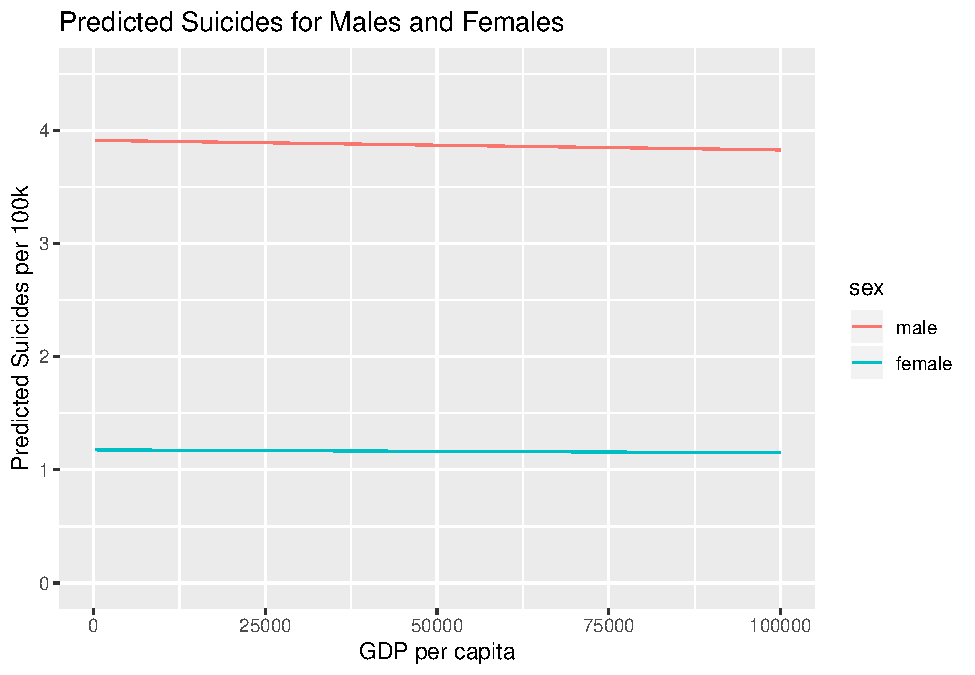
\includegraphics{An-Analysis-of-Suicide-Data_files/figure-latex/unnamed-chunk-4-1.pdf}

Interpretation of GDP per capita and sex:

GDP: for every \$1,000 increase in GDP per capita, holding all other
variables constant, we predict, on average, that the number of suicides
per 100k will decrease by 0.02\% (or multiply by e\^{}-.0002) (this
variable is not very significant in the model)

Sex: holding all other variables constant, on average, we predict that
the number of suicides per 100k will be 3.324 times greater for males
than that of females

\hypertarget{aggregate-data-model-selection-without-interaction}{%
\section{Aggregate Data Model Selection (without
interaction)}\label{aggregate-data-model-selection-without-interaction}}

\begin{Shaded}
\begin{Highlighting}[]
\CommentTok{# first let's look at the correlations between our numerical predictors... no significant correlations}
\KeywordTok{cor}\NormalTok{(}\KeywordTok{subset}\NormalTok{(aggregate.suicides, }\DataTypeTok{select =} \KeywordTok{c}\NormalTok{(Year, GDP.per.capita, Population, Suicides.per100)))}
\end{Highlighting}
\end{Shaded}

\begin{verbatim}
##                         Year GDP.per.capita  Population Suicides.per100
## Year             1.000000000     0.31062227 0.007685861     -0.06842743
## GDP.per.capita   0.310622267     1.00000000 0.086747489      0.03413896
## Population       0.007685861     0.08674749 1.000000000      0.08007144
## Suicides.per100 -0.068427431     0.03413896 0.080071440      1.00000000
\end{verbatim}

\begin{Shaded}
\begin{Highlighting}[]
\CommentTok{## Model with no transformations}
\NormalTok{agg.fit1 <-}\StringTok{ }\KeywordTok{lm}\NormalTok{(Suicides.per100 }\OperatorTok{~}\StringTok{ }\NormalTok{Development }\OperatorTok{+}\StringTok{ }\NormalTok{Region }\OperatorTok{+}\StringTok{ }\NormalTok{GDP.per.capita }\OperatorTok{+}\StringTok{ }\NormalTok{Population }\OperatorTok{+}\StringTok{ }\NormalTok{Year, }\DataTypeTok{data =}\NormalTok{ aggregate.suicides)}
\KeywordTok{summary}\NormalTok{(agg.fit1)}
\end{Highlighting}
\end{Shaded}

\begin{verbatim}
## 
## Call:
## lm(formula = Suicides.per100 ~ Development + Region + GDP.per.capita + 
##     Population + Year, data = aggregate.suicides)
## 
## Residuals:
##     Min      1Q  Median      3Q     Max 
## -17.870  -5.295  -1.152   3.282  33.034 
## 
## Coefficients:
##                              Estimate Std. Error t value Pr(>|t|)    
## (Intercept)                 9.311e+01  5.361e+01   1.737  0.08258 .  
## Developmentlow or very low -1.354e+00  2.156e+00  -0.628  0.53013    
## Developmentmedium          -9.179e-01  7.001e-01  -1.311  0.18998    
## Developmentunknown         -5.493e-01  5.648e-01  -0.972  0.33096    
## RegionAsia                 -8.073e-01  1.105e+00  -0.731  0.46490    
## RegionCaribbean             1.989e+00  1.051e+00   1.893  0.05856 .  
## RegionCentral America      -1.402e+00  1.184e+00  -1.184  0.23660    
## RegionEurope                1.012e+01  1.028e+00   9.846  < 2e-16 ***
## RegionNorth America         3.981e+00  1.453e+00   2.739  0.00622 ** 
## RegionOceania               4.355e+00  1.341e+00   3.247  0.00119 ** 
## RegionSouth America         2.927e+00  1.098e+00   2.666  0.00775 ** 
## GDP.per.capita             -5.620e-05  1.092e-05  -5.148 2.89e-07 ***
## Population                 -3.378e-09  5.226e-09  -0.646  0.51811    
## Year                       -4.235e-02  2.670e-02  -1.586  0.11290    
## ---
## Signif. codes:  0 '***' 0.001 '**' 0.01 '*' 0.05 '.' 0.1 ' ' 1
## 
## Residual standard error: 7.598 on 1937 degrees of freedom
##   (119 observations deleted due to missingness)
## Multiple R-squared:  0.2467, Adjusted R-squared:  0.2417 
## F-statistic:  48.8 on 13 and 1937 DF,  p-value: < 2.2e-16
\end{verbatim}

\begin{Shaded}
\begin{Highlighting}[]
\CommentTok{# there is heteroskedasticity and residuals are not normally distributed}
\KeywordTok{plot}\NormalTok{(agg.fit1, }\DecValTok{1}\NormalTok{)}
\end{Highlighting}
\end{Shaded}

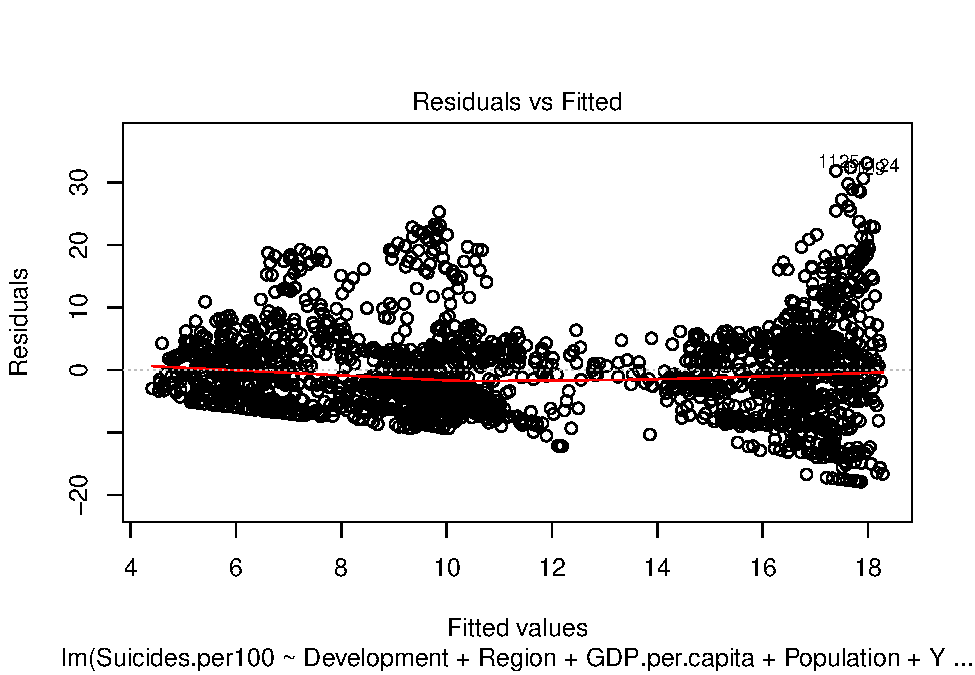
\includegraphics{An-Analysis-of-Suicide-Data_files/figure-latex/unnamed-chunk-5-1.pdf}

\begin{Shaded}
\begin{Highlighting}[]
\KeywordTok{plot}\NormalTok{(agg.fit1, }\DecValTok{2}\NormalTok{)}
\end{Highlighting}
\end{Shaded}

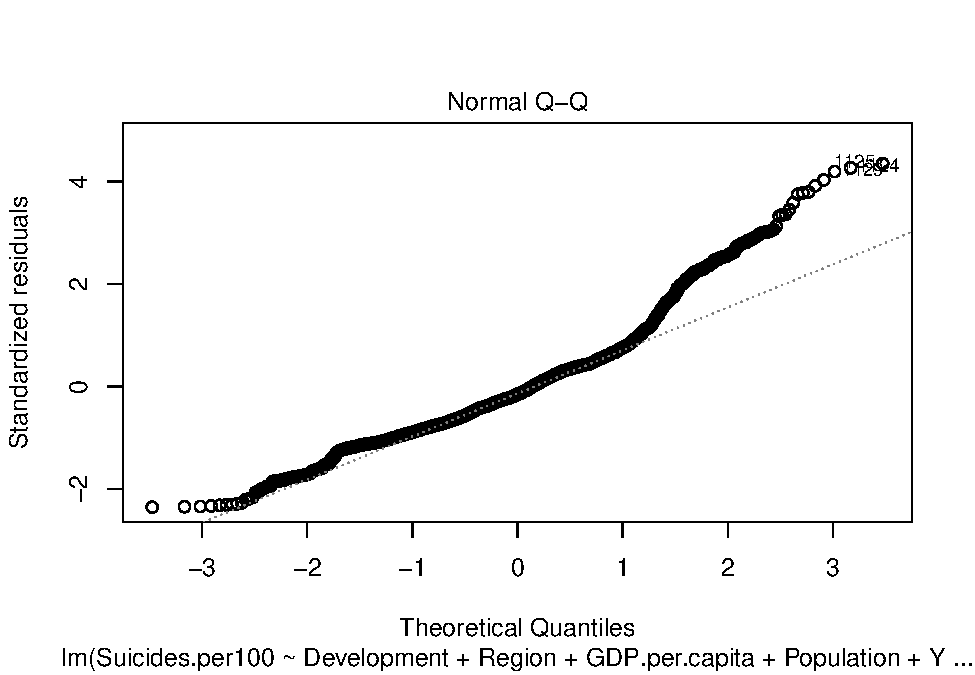
\includegraphics{An-Analysis-of-Suicide-Data_files/figure-latex/unnamed-chunk-5-2.pdf}

\begin{Shaded}
\begin{Highlighting}[]
\CommentTok{## Model with log(y+1) transformation}
\NormalTok{agg.fit2 <-}\StringTok{ }\KeywordTok{lm}\NormalTok{(}\KeywordTok{log}\NormalTok{(Suicides.per100 }\OperatorTok{+}\StringTok{ }\DecValTok{1}\NormalTok{) }\OperatorTok{~}\StringTok{ }\NormalTok{Development }\OperatorTok{+}\StringTok{ }\NormalTok{Region }\OperatorTok{+}\StringTok{ }\NormalTok{GDP.per.capita }\OperatorTok{+}\StringTok{ }\NormalTok{Population }\OperatorTok{+}\StringTok{ }\NormalTok{Year, }\DataTypeTok{data =}\NormalTok{ aggregate.suicides)}
\NormalTok{agg.fit2.sum <-}\StringTok{ }\KeywordTok{summary}\NormalTok{(agg.fit2)}

\CommentTok{# heteroskedasticity is fixed, but residuals are not normally distributed}
\KeywordTok{plot}\NormalTok{(agg.fit2, }\DecValTok{1}\NormalTok{)}
\end{Highlighting}
\end{Shaded}

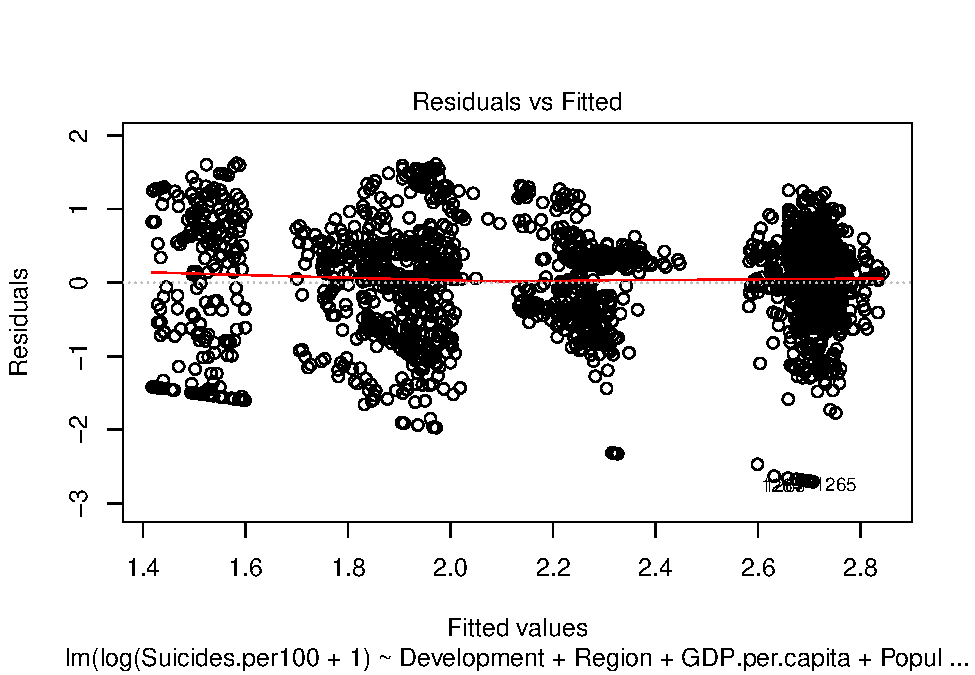
\includegraphics{An-Analysis-of-Suicide-Data_files/figure-latex/unnamed-chunk-5-3.pdf}

\begin{Shaded}
\begin{Highlighting}[]
\KeywordTok{plot}\NormalTok{(agg.fit2, }\DecValTok{2}\NormalTok{)}
\end{Highlighting}
\end{Shaded}

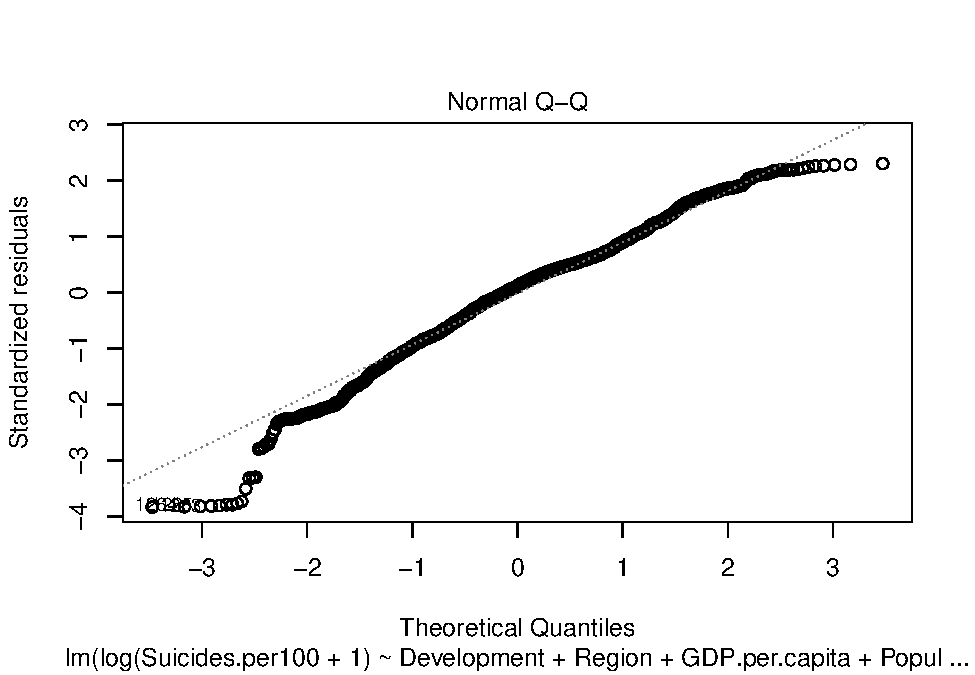
\includegraphics{An-Analysis-of-Suicide-Data_files/figure-latex/unnamed-chunk-5-4.pdf}

\begin{Shaded}
\begin{Highlighting}[]
\CommentTok{# since the normality assumption is broken, we should do bootstrapping for betas}
\NormalTok{n <-}\StringTok{ }\KeywordTok{nrow}\NormalTok{(aggregate.suicides)}
\NormalTok{i <-}\StringTok{ }\KeywordTok{sample}\NormalTok{(}\DecValTok{1}\OperatorTok{:}\NormalTok{n, n, }\DataTypeTok{replace=}\NormalTok{T)}
\KeywordTok{set.seed}\NormalTok{(}\DecValTok{12}\NormalTok{)}
\NormalTok{p.values <-}\StringTok{ }\KeywordTok{c}\NormalTok{()}
\NormalTok{confidence.lower <-}\StringTok{ }\KeywordTok{c}\NormalTok{()}
\NormalTok{confidence.upper <-}\StringTok{ }\KeywordTok{c}\NormalTok{()}
\NormalTok{beta.estimates <-}\StringTok{ }\KeywordTok{c}\NormalTok{()}

\ControlFlowTok{for}\NormalTok{ (index }\ControlFlowTok{in} \DecValTok{2}\OperatorTok{:}\DecValTok{14}\NormalTok{)\{}
\NormalTok{  beta1 <-}\StringTok{ }\ControlFlowTok{function}\NormalTok{(x,i) \{ }\KeywordTok{coef}\NormalTok{(}\KeywordTok{lm}\NormalTok{(}\KeywordTok{log}\NormalTok{(Suicides.per100 }\OperatorTok{+}\StringTok{ }\DecValTok{1}\NormalTok{) }\OperatorTok{~}\StringTok{ }\NormalTok{Development }\OperatorTok{+}\StringTok{ }\NormalTok{Region }\OperatorTok{+}\StringTok{ }\NormalTok{GDP.per.capita }\OperatorTok{+}\StringTok{ }\NormalTok{Population }\OperatorTok{+}\StringTok{ }\NormalTok{Year,}
                                   \DataTypeTok{data =}\NormalTok{ x,}
                                   \DataTypeTok{subset =}\NormalTok{ i))[index]\}}
  
  
\NormalTok{  res <-}\StringTok{ }\KeywordTok{boot}\NormalTok{(}\DataTypeTok{data =}\NormalTok{ aggregate.suicides,}
              \DataTypeTok{statistic =}\NormalTok{ beta1,}
              \DataTypeTok{R =} \DecValTok{1000}\NormalTok{)}
  
\NormalTok{  beta1.full <-}\StringTok{ }\KeywordTok{coef}\NormalTok{(}\KeywordTok{lm}\NormalTok{(}\KeywordTok{log}\NormalTok{(Suicides.per100 }\OperatorTok{+}\StringTok{ }\DecValTok{1}\NormalTok{) }\OperatorTok{~}\StringTok{ }\NormalTok{Development }\OperatorTok{+}\StringTok{ }\NormalTok{Region }\OperatorTok{+}\StringTok{ }\NormalTok{GDP.per.capita }\OperatorTok{+}\StringTok{ }\NormalTok{Population }\OperatorTok{+}\StringTok{ }\NormalTok{Year,}
                        \DataTypeTok{data=}\NormalTok{aggregate.suicides))[index]}
  
\NormalTok{  bias <-}\StringTok{ }\KeywordTok{mean}\NormalTok{(res}\OperatorTok{$}\NormalTok{t) }\OperatorTok{-}\StringTok{ }\NormalTok{beta1.full}
  
\NormalTok{  unbiased.est <-}\StringTok{ }\NormalTok{res}\OperatorTok{$}\NormalTok{t }\OperatorTok{-}\StringTok{ }\NormalTok{bias}
  
\NormalTok{  conf.low <-}\StringTok{ }\KeywordTok{quantile}\NormalTok{(unbiased.est, }\FloatTok{0.025}\NormalTok{)}
\NormalTok{  conf.up <-}\StringTok{ }\KeywordTok{quantile}\NormalTok{(unbiased.est, }\FloatTok{0.975}\NormalTok{)}
  
\NormalTok{  beta.H0 <-res}\OperatorTok{$}\NormalTok{t }\OperatorTok{-}\StringTok{ }\KeywordTok{mean}\NormalTok{(res}\OperatorTok{$}\NormalTok{t) }\OperatorTok{+}\StringTok{ }\NormalTok{bias}
  
\NormalTok{  p.val <-}\StringTok{ }\KeywordTok{mean}\NormalTok{(}\KeywordTok{abs}\NormalTok{(beta.H0) }\OperatorTok{>=}\StringTok{ }\KeywordTok{abs}\NormalTok{(beta1.full))}
  
\NormalTok{  beta.estimates <-}\StringTok{ }\KeywordTok{append}\NormalTok{(beta.estimates, beta1.full)}
\NormalTok{  p.values <-}\StringTok{ }\KeywordTok{append}\NormalTok{(p.values, p.val)}
\NormalTok{  confidence.lower <-}\StringTok{ }\KeywordTok{append}\NormalTok{(confidence.lower, conf.low)}
\NormalTok{  confidence.upper <-}\StringTok{ }\KeywordTok{append}\NormalTok{(confidence.upper, conf.up)}
  
  
\NormalTok{\}}

\NormalTok{boot.info2 <-}\StringTok{ }\KeywordTok{data.frame}\NormalTok{( beta.estimates, p.values)}
\KeywordTok{colnames}\NormalTok{(boot.info2) <-}\StringTok{ }\KeywordTok{c}\NormalTok{( }\StringTok{"Estimates"}\NormalTok{, }\StringTok{"P.value"}\NormalTok{)}
\CommentTok{# more accurate p-values}
\NormalTok{boot.info2}
\end{Highlighting}
\end{Shaded}

\begin{verbatim}
##                                Estimates P.value
## Developmentlow or very low -1.247389e-01   0.510
## Developmentmedium          -1.120734e-01   0.054
## Developmentunknown         -6.377532e-02   0.098
## RegionAsia                 -2.805231e-01   0.031
## RegionCaribbean             1.296387e-01   0.277
## RegionCentral America       5.333066e-02   0.656
## RegionEurope                8.841251e-01   0.000
## RegionNorth America         4.324709e-01   0.002
## RegionOceania               4.978520e-01   0.000
## RegionSouth America         4.331285e-01   0.000
## GDP.per.capita              2.540315e-07   0.755
## Population                  1.508152e-10   0.702
## Year                       -5.569984e-03   0.021
\end{verbatim}

\begin{Shaded}
\begin{Highlighting}[]
\CommentTok{# dataframe with old and new p-values}
\NormalTok{p.val.compare2 <-}\StringTok{ }\KeywordTok{data.frame}\NormalTok{(beta.estimates, agg.fit2.sum}\OperatorTok{$}\NormalTok{coefficients[}\DecValTok{2}\OperatorTok{:}\DecValTok{14}\NormalTok{,}\DecValTok{4}\NormalTok{], p.values)}
\KeywordTok{colnames}\NormalTok{(p.val.compare2) <-}\StringTok{ }\KeywordTok{c}\NormalTok{(}\StringTok{"estimates"}\NormalTok{, }\StringTok{"lm() p-values"}\NormalTok{, }\StringTok{"bootstrap p-values"}\NormalTok{)}

\NormalTok{p.val.compare2}
\end{Highlighting}
\end{Shaded}

\begin{verbatim}
##                                estimates lm() p-values bootstrap p-values
## Developmentlow or very low -1.247389e-01  5.339324e-01              0.510
## Developmentmedium          -1.120734e-01  8.538863e-02              0.054
## Developmentunknown         -6.377532e-02  2.249054e-01              0.098
## RegionAsia                 -2.805231e-01  6.377325e-03              0.031
## RegionCaribbean             1.296387e-01  1.848951e-01              0.277
## RegionCentral America       5.333066e-02  6.283205e-01              0.656
## RegionEurope                8.841251e-01  5.689075e-20              0.000
## RegionNorth America         4.324709e-01  1.401068e-03              0.002
## RegionOceania               4.978520e-01  6.816981e-05              0.000
## RegionSouth America         4.331285e-01  2.334599e-05              0.000
## GDP.per.capita              2.540315e-07  8.024701e-01              0.755
## Population                  1.508152e-10  7.563908e-01              0.702
## Year                       -5.569984e-03  2.503708e-02              0.021
\end{verbatim}

\begin{Shaded}
\begin{Highlighting}[]
\KeywordTok{AIC}\NormalTok{(agg.fit2)}
\end{Highlighting}
\end{Shaded}

\begin{verbatim}
## [1] 4197.765
\end{verbatim}

\begin{Shaded}
\begin{Highlighting}[]
\CommentTok{## Model with log(y) transformation but observations with 0 suicides are removed}
\NormalTok{agg.fit3 <-}\StringTok{ }\KeywordTok{lm}\NormalTok{(}\KeywordTok{log}\NormalTok{(Suicides.per100) }\OperatorTok{~}\StringTok{ }\NormalTok{Development }\OperatorTok{+}\StringTok{ }\NormalTok{Region }\OperatorTok{+}\StringTok{ }\NormalTok{GDP.per.capita }\OperatorTok{+}\StringTok{ }\NormalTok{Population }\OperatorTok{+}\StringTok{ }\NormalTok{Year, }\DataTypeTok{data =}\NormalTok{ agg.subset.rm)}
\NormalTok{agg.fit3.sum <-}\StringTok{ }\KeywordTok{summary}\NormalTok{(agg.fit3)}

\CommentTok{# heteroskedasticity is mosly fixed, but residuals are not normally distributed}
\KeywordTok{plot}\NormalTok{(agg.fit3, }\DecValTok{1}\NormalTok{)}
\end{Highlighting}
\end{Shaded}

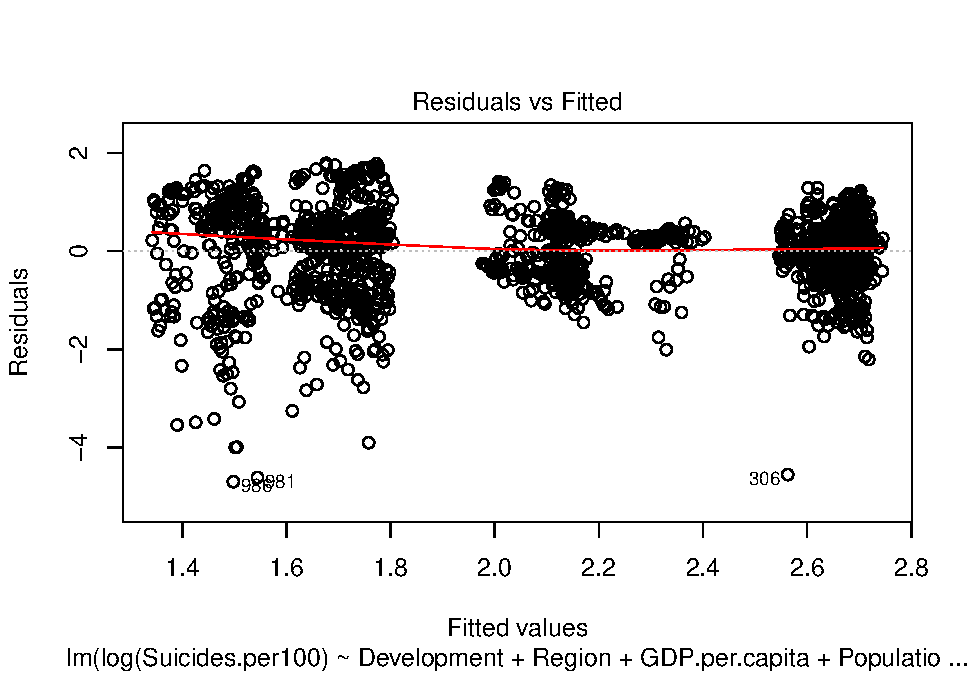
\includegraphics{An-Analysis-of-Suicide-Data_files/figure-latex/unnamed-chunk-6-1.pdf}

\begin{Shaded}
\begin{Highlighting}[]
\KeywordTok{plot}\NormalTok{(agg.fit3, }\DecValTok{2}\NormalTok{)}
\end{Highlighting}
\end{Shaded}

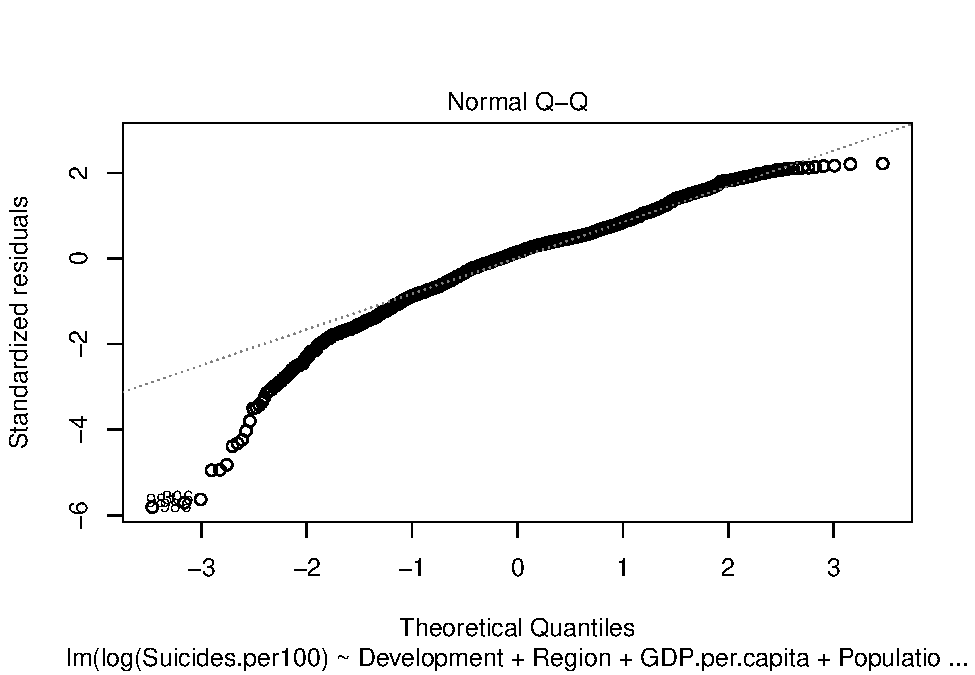
\includegraphics{An-Analysis-of-Suicide-Data_files/figure-latex/unnamed-chunk-6-2.pdf}

\begin{Shaded}
\begin{Highlighting}[]
\CommentTok{# since the normality assumption is broken, we should do bootstrapping for betas}
\NormalTok{n <-}\StringTok{ }\KeywordTok{nrow}\NormalTok{(agg.subset.rm)}
\NormalTok{i <-}\StringTok{ }\KeywordTok{sample}\NormalTok{(}\DecValTok{1}\OperatorTok{:}\NormalTok{n, n, }\DataTypeTok{replace=}\NormalTok{T)}
\KeywordTok{set.seed}\NormalTok{(}\DecValTok{12}\NormalTok{)}
\NormalTok{p.values <-}\StringTok{ }\KeywordTok{c}\NormalTok{()}
\NormalTok{confidence.lower <-}\StringTok{ }\KeywordTok{c}\NormalTok{()}
\NormalTok{confidence.upper <-}\StringTok{ }\KeywordTok{c}\NormalTok{()}
\NormalTok{beta.estimates <-}\StringTok{ }\KeywordTok{c}\NormalTok{()}

\ControlFlowTok{for}\NormalTok{ (index }\ControlFlowTok{in} \DecValTok{2}\OperatorTok{:}\DecValTok{14}\NormalTok{)\{}
\NormalTok{  beta1 <-}\StringTok{ }\ControlFlowTok{function}\NormalTok{(x,i) \{ }\KeywordTok{coef}\NormalTok{(}\KeywordTok{lm}\NormalTok{(}\KeywordTok{log}\NormalTok{(Suicides.per100) }\OperatorTok{~}\StringTok{ }\NormalTok{Development }\OperatorTok{+}\StringTok{ }\NormalTok{Region }\OperatorTok{+}\StringTok{ }\NormalTok{GDP.per.capita }\OperatorTok{+}\StringTok{ }\NormalTok{Population }\OperatorTok{+}\StringTok{ }\NormalTok{Year,}
                                   \DataTypeTok{data =}\NormalTok{ x,}
                                   \DataTypeTok{subset =}\NormalTok{ i))[index]\}}
  
  
\NormalTok{  res <-}\StringTok{ }\KeywordTok{boot}\NormalTok{(}\DataTypeTok{data =}\NormalTok{ agg.subset.rm,}
              \DataTypeTok{statistic =}\NormalTok{ beta1,}
              \DataTypeTok{R =} \DecValTok{1000}\NormalTok{)}
  
\NormalTok{  beta1.full <-}\StringTok{ }\KeywordTok{coef}\NormalTok{(}\KeywordTok{lm}\NormalTok{(}\KeywordTok{log}\NormalTok{(Suicides.per100) }\OperatorTok{~}\StringTok{ }\NormalTok{Development }\OperatorTok{+}\StringTok{ }\NormalTok{Region }\OperatorTok{+}\StringTok{ }\NormalTok{GDP.per.capita }\OperatorTok{+}\StringTok{ }\NormalTok{Population }\OperatorTok{+}\StringTok{ }\NormalTok{Year,}
                        \DataTypeTok{data=}\NormalTok{agg.subset.rm))[index]}
  
\NormalTok{  bias <-}\StringTok{ }\KeywordTok{mean}\NormalTok{(res}\OperatorTok{$}\NormalTok{t) }\OperatorTok{-}\StringTok{ }\NormalTok{beta1.full}
  
\NormalTok{  unbiased.est <-}\StringTok{ }\NormalTok{res}\OperatorTok{$}\NormalTok{t }\OperatorTok{-}\StringTok{ }\NormalTok{bias}
  
\NormalTok{  conf.low <-}\StringTok{ }\KeywordTok{quantile}\NormalTok{(unbiased.est, }\FloatTok{0.025}\NormalTok{)}
\NormalTok{  conf.up <-}\StringTok{ }\KeywordTok{quantile}\NormalTok{(unbiased.est, }\FloatTok{0.975}\NormalTok{)}
  
\NormalTok{  beta.H0 <-res}\OperatorTok{$}\NormalTok{t }\OperatorTok{-}\StringTok{ }\KeywordTok{mean}\NormalTok{(res}\OperatorTok{$}\NormalTok{t) }\OperatorTok{+}\StringTok{ }\NormalTok{bias}
  
\NormalTok{  p.val <-}\StringTok{ }\KeywordTok{mean}\NormalTok{(}\KeywordTok{abs}\NormalTok{(beta.H0) }\OperatorTok{>=}\StringTok{ }\KeywordTok{abs}\NormalTok{(beta1.full))}
  
\NormalTok{  beta.estimates <-}\StringTok{ }\KeywordTok{append}\NormalTok{(beta.estimates, beta1.full)}
\NormalTok{  p.values <-}\StringTok{ }\KeywordTok{append}\NormalTok{(p.values, p.val)}
\NormalTok{  confidence.lower <-}\StringTok{ }\KeywordTok{append}\NormalTok{(confidence.lower, conf.low)}
\NormalTok{  confidence.upper <-}\StringTok{ }\KeywordTok{append}\NormalTok{(confidence.upper, conf.up)}
  
  
\NormalTok{\}}

\NormalTok{boot.info3 <-}\StringTok{ }\KeywordTok{data.frame}\NormalTok{( beta.estimates, p.values)}
\KeywordTok{colnames}\NormalTok{(boot.info3) <-}\StringTok{ }\KeywordTok{c}\NormalTok{( }\StringTok{"Estimates"}\NormalTok{, }\StringTok{"P.value"}\NormalTok{)}
\CommentTok{# more accurate p-values}
\NormalTok{boot.info3}
\end{Highlighting}
\end{Shaded}

\begin{verbatim}
##                                Estimates P.value
## Developmentlow or very low -1.179284e-01   0.634
## Developmentmedium          -1.260214e-01   0.084
## Developmentunknown         -3.969856e-02   0.378
## RegionAsia                  2.510204e-02   0.875
## RegionCaribbean             2.750080e-01   0.108
## RegionCentral America       1.921020e-01   0.251
## RegionEurope                1.201192e+00   0.000
## RegionNorth America         7.085138e-01   0.000
## RegionOceania               8.521374e-01   0.000
## RegionSouth America         6.515398e-01   0.000
## GDP.per.capita             -8.717889e-07   0.329
## Population                 -1.062931e-10   0.825
## Year                       -3.418648e-03   0.224
\end{verbatim}

\begin{Shaded}
\begin{Highlighting}[]
\CommentTok{# dataframe with old and new p-values}
\NormalTok{p.val.compare3 <-}\StringTok{ }\KeywordTok{data.frame}\NormalTok{(beta.estimates, agg.fit3.sum}\OperatorTok{$}\NormalTok{coefficients[}\DecValTok{2}\OperatorTok{:}\DecValTok{14}\NormalTok{,}\DecValTok{4}\NormalTok{], p.values)}
\KeywordTok{colnames}\NormalTok{(p.val.compare3) <-}\StringTok{ }\KeywordTok{c}\NormalTok{(}\StringTok{"estimates"}\NormalTok{, }\StringTok{"lm() p-values"}\NormalTok{, }\StringTok{"bootstrap p-values"}\NormalTok{)}

\NormalTok{p.val.compare3}
\end{Highlighting}
\end{Shaded}

\begin{verbatim}
##                                estimates lm() p-values bootstrap p-values
## Developmentlow or very low -1.179284e-01  6.088373e-01              0.634
## Developmentmedium          -1.260214e-01  9.476094e-02              0.084
## Developmentunknown         -3.969856e-02  5.112396e-01              0.378
## RegionAsia                  2.510204e-02  8.354053e-01              0.875
## RegionCaribbean             2.750080e-01  1.452276e-02              0.108
## RegionCentral America       1.921020e-01  1.291050e-01              0.251
## RegionEurope                1.201192e+00  5.482558e-27              0.000
## RegionNorth America         7.085138e-01  5.455469e-06              0.000
## RegionOceania               8.521374e-01  4.766926e-09              0.000
## RegionSouth America         6.515398e-01  3.207376e-08              0.000
## GDP.per.capita             -8.717889e-07  4.577292e-01              0.329
## Population                 -1.062931e-10  8.491618e-01              0.825
## Year                       -3.418648e-03  2.379932e-01              0.224
\end{verbatim}

\begin{Shaded}
\begin{Highlighting}[]
\KeywordTok{AIC}\NormalTok{(agg.fit3)}
\end{Highlighting}
\end{Shaded}

\begin{verbatim}
## [1] 4610.243
\end{verbatim}

Considering the more practical performance of the model that removed the
observations with 0 suicides, I am doing the same with aggregate suicide
data\ldots{} there is even less missing data. The R\^{}2 is much better
for the log(y) model as compared to the log(y+1) model too. Again,
log(y+1) is modeling a different response than that of log(y) and the
results are poor. The predicted amount of suicides are often much larger
than what they should actually be due to the transformation

\begin{Shaded}
\begin{Highlighting}[]
\CommentTok{## Removing insignificant predictors and making a new model}
\CommentTok{# development seems to add too much complication to the model and may not be significant enough... population is insignificant as well}
\CommentTok{## Model with log(y) transformation but observations with 0 suicides are removed}
\NormalTok{agg.fit4 <-}\StringTok{ }\KeywordTok{lm}\NormalTok{(}\KeywordTok{log}\NormalTok{(Suicides.per100) }\OperatorTok{~}\StringTok{ }\NormalTok{Region }\OperatorTok{+}\StringTok{ }\NormalTok{GDP.per.capita }\OperatorTok{+}\StringTok{ }\NormalTok{Year, }\DataTypeTok{data =}\NormalTok{ agg.subset.rm)}
\NormalTok{agg.fit4.sum <-}\StringTok{ }\KeywordTok{summary}\NormalTok{(agg.fit4)}

\CommentTok{# heteroskedasticity is mosly fixed, but residuals are not normally distributed}
\KeywordTok{plot}\NormalTok{(agg.fit4, }\DecValTok{1}\NormalTok{)}
\end{Highlighting}
\end{Shaded}

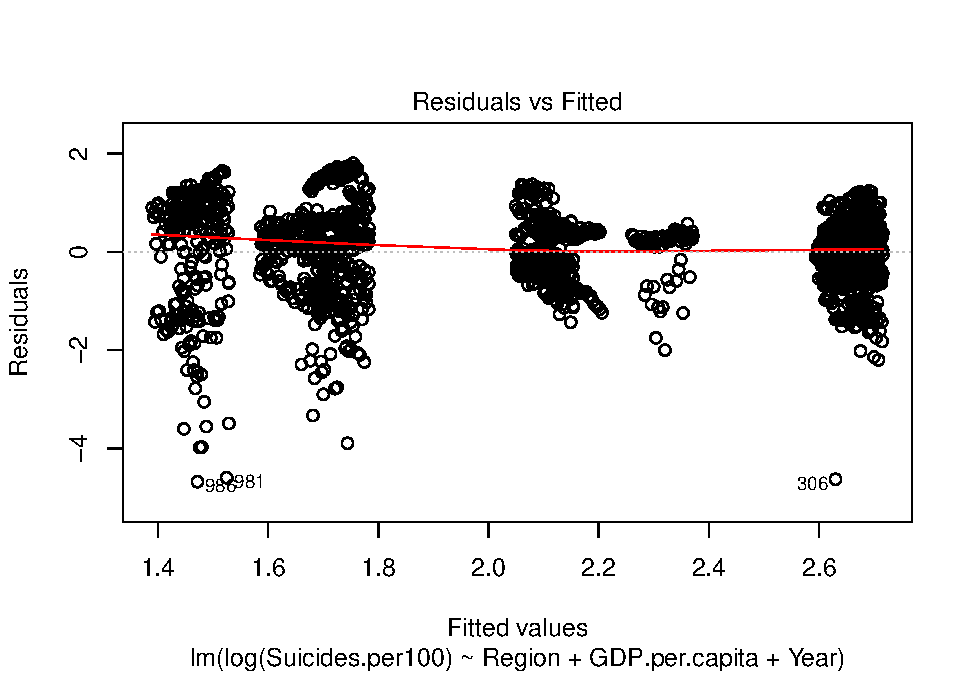
\includegraphics{An-Analysis-of-Suicide-Data_files/figure-latex/unnamed-chunk-7-1.pdf}

\begin{Shaded}
\begin{Highlighting}[]
\KeywordTok{plot}\NormalTok{(agg.fit4, }\DecValTok{2}\NormalTok{)}
\end{Highlighting}
\end{Shaded}

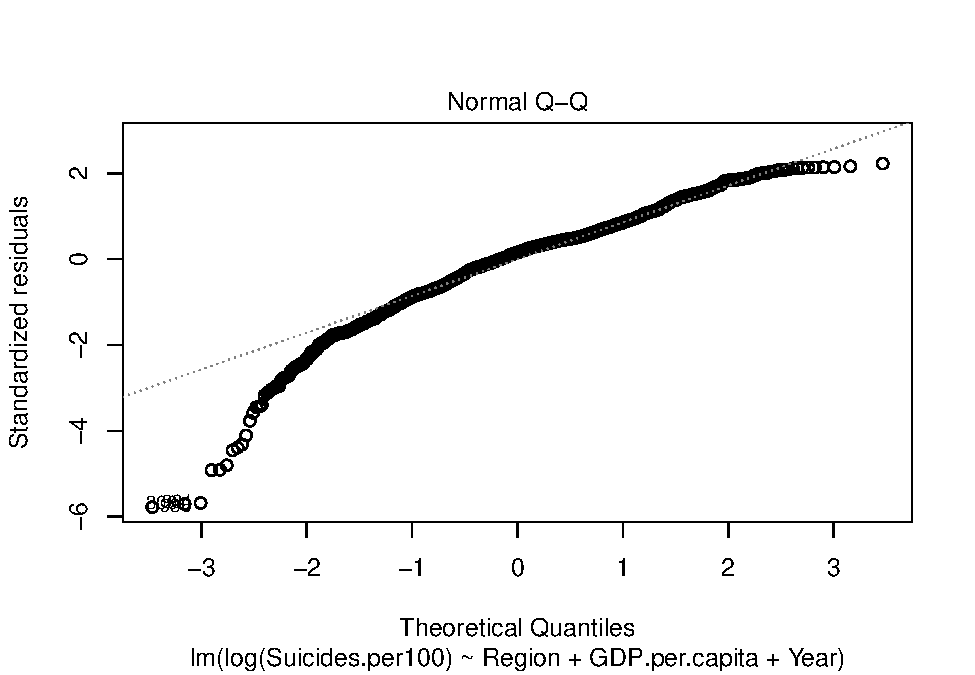
\includegraphics{An-Analysis-of-Suicide-Data_files/figure-latex/unnamed-chunk-7-2.pdf}

\begin{Shaded}
\begin{Highlighting}[]
\CommentTok{# since the normality assumption is broken, we should do bootstrapping for betas}
\NormalTok{n <-}\StringTok{ }\KeywordTok{nrow}\NormalTok{(agg.subset.rm)}
\NormalTok{i <-}\StringTok{ }\KeywordTok{sample}\NormalTok{(}\DecValTok{1}\OperatorTok{:}\NormalTok{n, n, }\DataTypeTok{replace=}\NormalTok{T)}
\KeywordTok{set.seed}\NormalTok{(}\DecValTok{12}\NormalTok{)}
\NormalTok{p.values <-}\StringTok{ }\KeywordTok{c}\NormalTok{()}
\NormalTok{confidence.lower <-}\StringTok{ }\KeywordTok{c}\NormalTok{()}
\NormalTok{confidence.upper <-}\StringTok{ }\KeywordTok{c}\NormalTok{()}
\NormalTok{beta.estimates <-}\StringTok{ }\KeywordTok{c}\NormalTok{()}

\ControlFlowTok{for}\NormalTok{ (index }\ControlFlowTok{in} \DecValTok{2}\OperatorTok{:}\DecValTok{10}\NormalTok{)\{}
\NormalTok{  beta1 <-}\StringTok{ }\ControlFlowTok{function}\NormalTok{(x,i) \{ }\KeywordTok{coef}\NormalTok{(}\KeywordTok{lm}\NormalTok{(}\KeywordTok{log}\NormalTok{(Suicides.per100) }\OperatorTok{~}\StringTok{ }\NormalTok{Region }\OperatorTok{+}\StringTok{ }\NormalTok{GDP.per.capita }\OperatorTok{+}\StringTok{ }\NormalTok{Year,}
                                   \DataTypeTok{data =}\NormalTok{ x,}
                                   \DataTypeTok{subset =}\NormalTok{ i))[index]\}}
  
  
\NormalTok{  res <-}\StringTok{ }\KeywordTok{boot}\NormalTok{(}\DataTypeTok{data =}\NormalTok{ agg.subset.rm,}
              \DataTypeTok{statistic =}\NormalTok{ beta1,}
              \DataTypeTok{R =} \DecValTok{1000}\NormalTok{)}
  
\NormalTok{  beta1.full <-}\StringTok{ }\KeywordTok{coef}\NormalTok{(}\KeywordTok{lm}\NormalTok{(}\KeywordTok{log}\NormalTok{(Suicides.per100) }\OperatorTok{~}\StringTok{ }\NormalTok{Region }\OperatorTok{+}\StringTok{ }\NormalTok{GDP.per.capita }\OperatorTok{+}\StringTok{ }\NormalTok{Year,}
                        \DataTypeTok{data=}\NormalTok{agg.subset.rm))[index]}
  
\NormalTok{  bias <-}\StringTok{ }\KeywordTok{mean}\NormalTok{(res}\OperatorTok{$}\NormalTok{t) }\OperatorTok{-}\StringTok{ }\NormalTok{beta1.full}
  
\NormalTok{  unbiased.est <-}\StringTok{ }\NormalTok{res}\OperatorTok{$}\NormalTok{t }\OperatorTok{-}\StringTok{ }\NormalTok{bias}
  
\NormalTok{  conf.low <-}\StringTok{ }\KeywordTok{quantile}\NormalTok{(unbiased.est, }\FloatTok{0.025}\NormalTok{)}
\NormalTok{  conf.up <-}\StringTok{ }\KeywordTok{quantile}\NormalTok{(unbiased.est, }\FloatTok{0.975}\NormalTok{)}
  
\NormalTok{  beta.H0 <-res}\OperatorTok{$}\NormalTok{t }\OperatorTok{-}\StringTok{ }\KeywordTok{mean}\NormalTok{(res}\OperatorTok{$}\NormalTok{t) }\OperatorTok{+}\StringTok{ }\NormalTok{bias}
  
\NormalTok{  p.val <-}\StringTok{ }\KeywordTok{mean}\NormalTok{(}\KeywordTok{abs}\NormalTok{(beta.H0) }\OperatorTok{>=}\StringTok{ }\KeywordTok{abs}\NormalTok{(beta1.full))}
  
\NormalTok{  beta.estimates <-}\StringTok{ }\KeywordTok{append}\NormalTok{(beta.estimates, beta1.full)}
\NormalTok{  p.values <-}\StringTok{ }\KeywordTok{append}\NormalTok{(p.values, p.val)}
\NormalTok{  confidence.lower <-}\StringTok{ }\KeywordTok{append}\NormalTok{(confidence.lower, conf.low)}
\NormalTok{  confidence.upper <-}\StringTok{ }\KeywordTok{append}\NormalTok{(confidence.upper, conf.up)}
  
  
\NormalTok{\}}

\NormalTok{boot.info4 <-}\StringTok{ }\KeywordTok{data.frame}\NormalTok{( beta.estimates, p.values)}
\KeywordTok{colnames}\NormalTok{(boot.info4) <-}\StringTok{ }\KeywordTok{c}\NormalTok{( }\StringTok{"Estimates"}\NormalTok{, }\StringTok{"P.value"}\NormalTok{)}
\CommentTok{# more accurate p-values}
\NormalTok{boot.info4}
\end{Highlighting}
\end{Shaded}

\begin{verbatim}
##                           Estimates P.value
## RegionAsia             3.216013e-02   0.850
## RegionCaribbean        2.858310e-01   0.074
## RegionCentral America  1.924171e-01   0.243
## RegionEurope           1.218853e+00   0.000
## RegionNorth America    7.096179e-01   0.000
## RegionOceania          8.765214e-01   0.000
## RegionSouth America    6.567108e-01   0.000
## GDP.per.capita        -1.936818e-07   0.833
## Year                  -4.051387e-03   0.125
\end{verbatim}

\begin{Shaded}
\begin{Highlighting}[]
\CommentTok{# dataframe with old and new p-values}
\NormalTok{p.val.compare4 <-}\StringTok{ }\KeywordTok{data.frame}\NormalTok{(beta.estimates, agg.fit4.sum}\OperatorTok{$}\NormalTok{coefficients[}\DecValTok{2}\OperatorTok{:}\DecValTok{10}\NormalTok{,}\DecValTok{4}\NormalTok{], p.values)}
\KeywordTok{colnames}\NormalTok{(p.val.compare4) <-}\StringTok{ }\KeywordTok{c}\NormalTok{(}\StringTok{"estimates"}\NormalTok{, }\StringTok{"lm() p-values"}\NormalTok{, }\StringTok{"bootstrap p-values"}\NormalTok{)}

\NormalTok{p.val.compare4}
\end{Highlighting}
\end{Shaded}

\begin{verbatim}
##                           estimates lm() p-values bootstrap p-values
## RegionAsia             3.216013e-02  7.895855e-01              0.850
## RegionCaribbean        2.858310e-01  1.086063e-02              0.074
## RegionCentral America  1.924171e-01  1.268452e-01              0.243
## RegionEurope           1.218853e+00  5.723485e-28              0.000
## RegionNorth America    7.096179e-01  5.587265e-07              0.000
## RegionOceania          8.765214e-01  1.431916e-09              0.000
## RegionSouth America    6.567108e-01  2.135044e-08              0.000
## GDP.per.capita        -1.936818e-07  8.586924e-01              0.833
## Year                  -4.051387e-03  1.387656e-01              0.125
\end{verbatim}

\begin{Shaded}
\begin{Highlighting}[]
\KeywordTok{AIC}\NormalTok{(agg.fit4)}
\end{Highlighting}
\end{Shaded}

\begin{verbatim}
## [1] 4605.724
\end{verbatim}

AIC of this model is marginally better that the one with population and
development, but it may setup for a good interaction effect. R\^{}2 is
about the same.

\hypertarget{final-model-without-interaction}{%
\subsection{Final Model without
interaction}\label{final-model-without-interaction}}

\begin{Shaded}
\begin{Highlighting}[]
\NormalTok{agg.fit4.sum}
\end{Highlighting}
\end{Shaded}

\begin{verbatim}
## 
## Call:
## lm(formula = log(Suicides.per100) ~ Region + GDP.per.capita + 
##     Year, data = agg.subset.rm)
## 
## Residuals:
##     Min      1Q  Median      3Q     Max 
## -4.6762 -0.4640  0.1259  0.4729  1.8037 
## 
## Coefficients:
##                         Estimate Std. Error t value Pr(>|t|)    
## (Intercept)            9.559e+00  5.483e+00   1.743   0.0814 .  
## RegionAsia             3.216e-02  1.205e-01   0.267   0.7896    
## RegionCaribbean        2.858e-01  1.121e-01   2.550   0.0109 *  
## RegionCentral America  1.924e-01  1.260e-01   1.527   0.1268    
## RegionEurope           1.219e+00  1.094e-01  11.142  < 2e-16 ***
## RegionNorth America    7.096e-01  1.413e-01   5.022 5.59e-07 ***
## RegionOceania          8.765e-01  1.441e-01   6.082 1.43e-09 ***
## RegionSouth America    6.567e-01  1.168e-01   5.625 2.14e-08 ***
## GDP.per.capita        -1.937e-07  1.088e-06  -0.178   0.8587    
## Year                  -4.051e-03  2.736e-03  -1.481   0.1388    
## ---
## Signif. codes:  0 '***' 0.001 '**' 0.01 '*' 0.05 '.' 0.1 ' ' 1
## 
## Residual standard error: 0.8116 on 1888 degrees of freedom
##   (116 observations deleted due to missingness)
## Multiple R-squared:  0.2531, Adjusted R-squared:  0.2496 
## F-statistic:  71.1 on 9 and 1888 DF,  p-value: < 2.2e-16
\end{verbatim}

\begin{Shaded}
\begin{Highlighting}[]
\NormalTok{p.val.compare4}
\end{Highlighting}
\end{Shaded}

\begin{verbatim}
##                           estimates lm() p-values bootstrap p-values
## RegionAsia             3.216013e-02  7.895855e-01              0.850
## RegionCaribbean        2.858310e-01  1.086063e-02              0.074
## RegionCentral America  1.924171e-01  1.268452e-01              0.243
## RegionEurope           1.218853e+00  5.723485e-28              0.000
## RegionNorth America    7.096179e-01  5.587265e-07              0.000
## RegionOceania          8.765214e-01  1.431916e-09              0.000
## RegionSouth America    6.567108e-01  2.135044e-08              0.000
## GDP.per.capita        -1.936818e-07  8.586924e-01              0.833
## Year                  -4.051387e-03  1.387656e-01              0.125
\end{verbatim}

\begin{Shaded}
\begin{Highlighting}[]
\KeywordTok{AIC}\NormalTok{(agg.fit4)}
\end{Highlighting}
\end{Shaded}

\begin{verbatim}
## [1] 4605.724
\end{verbatim}

\hypertarget{aggregate-data-model-selection-with-interaction}{%
\section{Aggregate Data Model Selection (with
interaction)}\label{aggregate-data-model-selection-with-interaction}}

\begin{Shaded}
\begin{Highlighting}[]
\CommentTok{## Interaction between GDP and Region}
\NormalTok{agg.fit5 <-}\StringTok{ }\KeywordTok{lm}\NormalTok{(}\KeywordTok{log}\NormalTok{(Suicides.per100) }\OperatorTok{~}\StringTok{ }\NormalTok{Region }\OperatorTok{+}\StringTok{ }\NormalTok{GDP.per.capita }\OperatorTok{+}\StringTok{ }\NormalTok{Year }\OperatorTok{+}\StringTok{ }\NormalTok{GDP.per.capita}\OperatorTok{:}\NormalTok{Region, }\DataTypeTok{data =}\NormalTok{ agg.subset.rm)}
\NormalTok{agg.fit5.sum <-}\StringTok{ }\KeywordTok{summary}\NormalTok{(agg.fit5)}

\CommentTok{# heteroskedasticity is mosly fixed, but residuals are not normally distributed}
\KeywordTok{plot}\NormalTok{(agg.fit5, }\DecValTok{1}\NormalTok{)}
\end{Highlighting}
\end{Shaded}

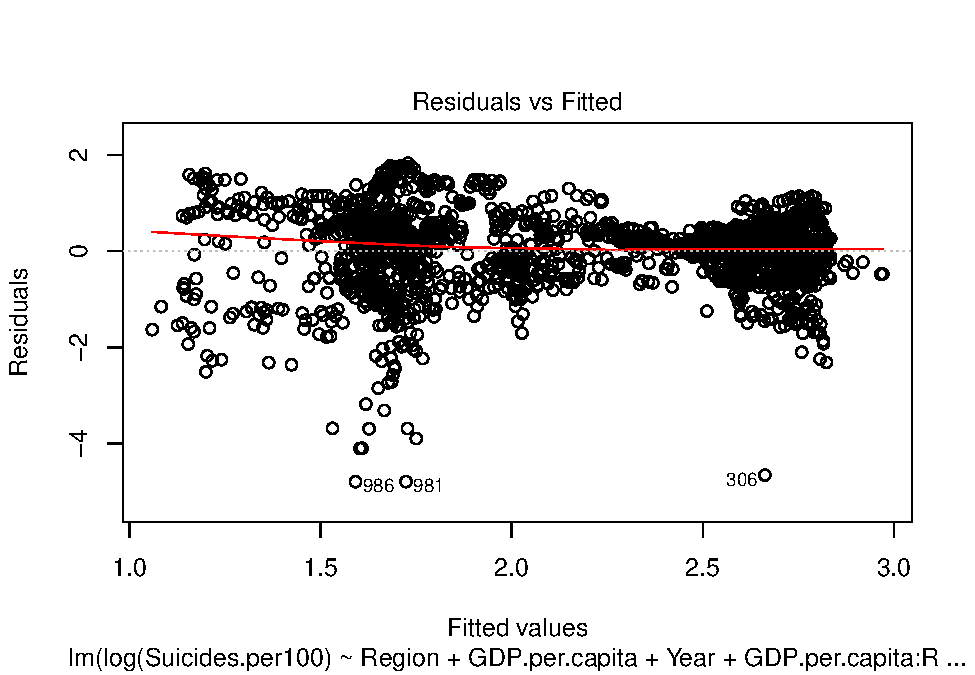
\includegraphics{An-Analysis-of-Suicide-Data_files/figure-latex/unnamed-chunk-9-1.pdf}

\begin{Shaded}
\begin{Highlighting}[]
\KeywordTok{plot}\NormalTok{(agg.fit5, }\DecValTok{2}\NormalTok{)}
\end{Highlighting}
\end{Shaded}

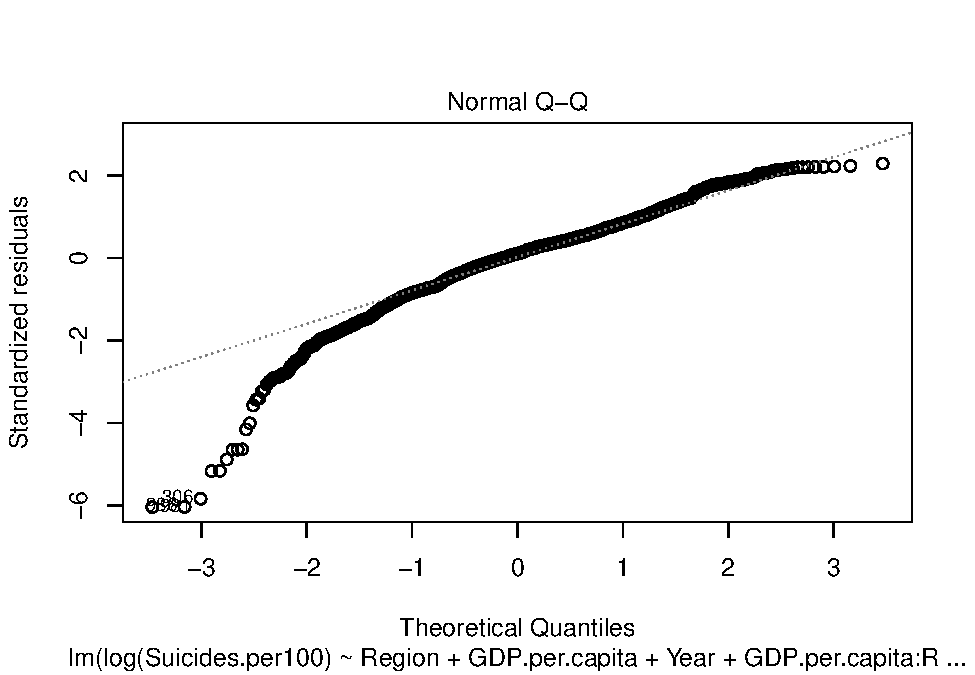
\includegraphics{An-Analysis-of-Suicide-Data_files/figure-latex/unnamed-chunk-9-2.pdf}

\begin{Shaded}
\begin{Highlighting}[]
\CommentTok{# since the normality assumption is broken, we should do bootstrapping for betas}
\NormalTok{n <-}\StringTok{ }\KeywordTok{nrow}\NormalTok{(agg.subset.rm)}
\NormalTok{i <-}\StringTok{ }\KeywordTok{sample}\NormalTok{(}\DecValTok{1}\OperatorTok{:}\NormalTok{n, n, }\DataTypeTok{replace=}\NormalTok{T)}
\KeywordTok{set.seed}\NormalTok{(}\DecValTok{12}\NormalTok{)}
\NormalTok{p.values <-}\StringTok{ }\KeywordTok{c}\NormalTok{()}
\NormalTok{confidence.lower <-}\StringTok{ }\KeywordTok{c}\NormalTok{()}
\NormalTok{confidence.upper <-}\StringTok{ }\KeywordTok{c}\NormalTok{()}
\NormalTok{beta.estimates <-}\StringTok{ }\KeywordTok{c}\NormalTok{()}

\ControlFlowTok{for}\NormalTok{ (index }\ControlFlowTok{in} \DecValTok{2}\OperatorTok{:}\DecValTok{17}\NormalTok{)\{}
\NormalTok{  beta1 <-}\StringTok{ }\ControlFlowTok{function}\NormalTok{(x,i) \{ }\KeywordTok{coef}\NormalTok{(}\KeywordTok{lm}\NormalTok{(}\KeywordTok{log}\NormalTok{(Suicides.per100) }\OperatorTok{~}\StringTok{ }\NormalTok{Region }\OperatorTok{+}\StringTok{ }\NormalTok{GDP.per.capita }\OperatorTok{+}\StringTok{ }\NormalTok{Year }\OperatorTok{+}\StringTok{ }\NormalTok{GDP.per.capita}\OperatorTok{:}\NormalTok{Region,}
                                   \DataTypeTok{data =}\NormalTok{ x,}
                                   \DataTypeTok{subset =}\NormalTok{ i))[index]\}}
  
  
\NormalTok{  res <-}\StringTok{ }\KeywordTok{boot}\NormalTok{(}\DataTypeTok{data =}\NormalTok{ agg.subset.rm,}
              \DataTypeTok{statistic =}\NormalTok{ beta1,}
              \DataTypeTok{R =} \DecValTok{1000}\NormalTok{)}
  
\NormalTok{  beta1.full <-}\StringTok{ }\KeywordTok{coef}\NormalTok{(}\KeywordTok{lm}\NormalTok{(}\KeywordTok{log}\NormalTok{(Suicides.per100) }\OperatorTok{~}\StringTok{ }\NormalTok{Region }\OperatorTok{+}\StringTok{ }\NormalTok{GDP.per.capita }\OperatorTok{+}\StringTok{ }\NormalTok{Year }\OperatorTok{+}\StringTok{ }\NormalTok{GDP.per.capita}\OperatorTok{:}\NormalTok{Region,}
                        \DataTypeTok{data=}\NormalTok{agg.subset.rm))[index]}
  
\NormalTok{  bias <-}\StringTok{ }\KeywordTok{mean}\NormalTok{(res}\OperatorTok{$}\NormalTok{t) }\OperatorTok{-}\StringTok{ }\NormalTok{beta1.full}
  
\NormalTok{  unbiased.est <-}\StringTok{ }\NormalTok{res}\OperatorTok{$}\NormalTok{t }\OperatorTok{-}\StringTok{ }\NormalTok{bias}
  
\NormalTok{  conf.low <-}\StringTok{ }\KeywordTok{quantile}\NormalTok{(unbiased.est, }\FloatTok{0.025}\NormalTok{)}
\NormalTok{  conf.up <-}\StringTok{ }\KeywordTok{quantile}\NormalTok{(unbiased.est, }\FloatTok{0.975}\NormalTok{)}
  
\NormalTok{  beta.H0 <-res}\OperatorTok{$}\NormalTok{t }\OperatorTok{-}\StringTok{ }\KeywordTok{mean}\NormalTok{(res}\OperatorTok{$}\NormalTok{t) }\OperatorTok{+}\StringTok{ }\NormalTok{bias}
  
\NormalTok{  p.val <-}\StringTok{ }\KeywordTok{mean}\NormalTok{(}\KeywordTok{abs}\NormalTok{(beta.H0) }\OperatorTok{>=}\StringTok{ }\KeywordTok{abs}\NormalTok{(beta1.full))}
  
\NormalTok{  beta.estimates <-}\StringTok{ }\KeywordTok{append}\NormalTok{(beta.estimates, beta1.full)}
\NormalTok{  p.values <-}\StringTok{ }\KeywordTok{append}\NormalTok{(p.values, p.val)}
\NormalTok{  confidence.lower <-}\StringTok{ }\KeywordTok{append}\NormalTok{(confidence.lower, conf.low)}
\NormalTok{  confidence.upper <-}\StringTok{ }\KeywordTok{append}\NormalTok{(confidence.upper, conf.up)}
  
  
\NormalTok{\}}

\NormalTok{boot.info5 <-}\StringTok{ }\KeywordTok{data.frame}\NormalTok{( beta.estimates, p.values)}
\KeywordTok{colnames}\NormalTok{(boot.info5) <-}\StringTok{ }\KeywordTok{c}\NormalTok{( }\StringTok{"Estimates"}\NormalTok{, }\StringTok{"P.value"}\NormalTok{)}
\CommentTok{# more accurate p-values}
\NormalTok{boot.info5}
\end{Highlighting}
\end{Shaded}

\begin{verbatim}
##                                          Estimates P.value
## RegionAsia                            8.438418e-01   0.051
## RegionCaribbean                       8.652377e-01   0.036
## RegionCentral America                 6.915980e-01   0.089
## RegionEurope                          1.925448e+00   0.000
## RegionNorth America                   5.893887e-01   0.166
## RegionOceania                         1.165874e+00   0.005
## RegionSouth America                   1.038377e+00   0.013
## GDP.per.capita                        8.567196e-05   0.018
## Year                                 -7.690527e-03   0.002
## RegionAsia:GDP.per.capita            -1.000537e-04   0.015
## RegionCaribbean:GDP.per.capita       -8.246098e-05   0.040
## RegionCentral America:GDP.per.capita -5.472676e-05   0.185
## RegionEurope:GDP.per.capita          -8.875707e-05   0.010
## RegionNorth America:GDP.per.capita   -5.905528e-05   0.115
## RegionOceania:GDP.per.capita         -7.108485e-05   0.068
## RegionSouth America:GDP.per.capita   -4.156215e-05   0.279
\end{verbatim}

\begin{Shaded}
\begin{Highlighting}[]
\CommentTok{# dataframe with old and new p-values}
\NormalTok{p.val.compare5 <-}\StringTok{ }\KeywordTok{data.frame}\NormalTok{(beta.estimates, agg.fit5.sum}\OperatorTok{$}\NormalTok{coefficients[}\DecValTok{2}\OperatorTok{:}\DecValTok{17}\NormalTok{,}\DecValTok{4}\NormalTok{], p.values)}
\KeywordTok{colnames}\NormalTok{(p.val.compare5) <-}\StringTok{ }\KeywordTok{c}\NormalTok{(}\StringTok{"estimates"}\NormalTok{, }\StringTok{"lm() p-values"}\NormalTok{, }\StringTok{"bootstrap p-values"}\NormalTok{)}

\NormalTok{p.val.compare5}
\end{Highlighting}
\end{Shaded}

\begin{verbatim}
##                                          estimates lm() p-values
## RegionAsia                            8.438418e-01  9.960212e-04
## RegionCaribbean                       8.652377e-01  3.367675e-04
## RegionCentral America                 6.915980e-01  1.013530e-02
## RegionEurope                          1.925448e+00  1.271913e-15
## RegionNorth America                   5.893887e-01  4.282314e-02
## RegionOceania                         1.165874e+00  3.174611e-05
## RegionSouth America                   1.038377e+00  3.782845e-05
## GDP.per.capita                        8.567196e-05  2.894590e-03
## Year                                 -7.690527e-03  6.288511e-03
## RegionAsia:GDP.per.capita            -1.000537e-04  6.560624e-04
## RegionCaribbean:GDP.per.capita       -8.246098e-05  4.176855e-03
## RegionCentral America:GDP.per.capita -5.472676e-05  1.557719e-01
## RegionEurope:GDP.per.capita          -8.875707e-05  2.018367e-03
## RegionNorth America:GDP.per.capita   -5.905528e-05  4.277041e-02
## RegionOceania:GDP.per.capita         -7.108485e-05  1.468454e-02
## RegionSouth America:GDP.per.capita   -4.156215e-05  1.856278e-01
##                                      bootstrap p-values
## RegionAsia                                        0.051
## RegionCaribbean                                   0.036
## RegionCentral America                             0.089
## RegionEurope                                      0.000
## RegionNorth America                               0.166
## RegionOceania                                     0.005
## RegionSouth America                               0.013
## GDP.per.capita                                    0.018
## Year                                              0.002
## RegionAsia:GDP.per.capita                         0.015
## RegionCaribbean:GDP.per.capita                    0.040
## RegionCentral America:GDP.per.capita              0.185
## RegionEurope:GDP.per.capita                       0.010
## RegionNorth America:GDP.per.capita                0.115
## RegionOceania:GDP.per.capita                      0.068
## RegionSouth America:GDP.per.capita                0.279
\end{verbatim}

\begin{Shaded}
\begin{Highlighting}[]
\KeywordTok{AIC}\NormalTok{(agg.fit5)}
\end{Highlighting}
\end{Shaded}

\begin{verbatim}
## [1] 4553.103
\end{verbatim}

\begin{Shaded}
\begin{Highlighting}[]
\CommentTok{## Interaction between Year and Region}
\NormalTok{agg.fit6 <-}\StringTok{ }\KeywordTok{lm}\NormalTok{(}\KeywordTok{log}\NormalTok{(Suicides.per100) }\OperatorTok{~}\StringTok{ }\NormalTok{Region }\OperatorTok{+}\StringTok{ }\NormalTok{GDP.per.capita }\OperatorTok{+}\StringTok{ }\NormalTok{Year }\OperatorTok{+}\StringTok{ }\NormalTok{Year}\OperatorTok{:}\NormalTok{Region, }\DataTypeTok{data =}\NormalTok{ agg.subset.rm)}
\NormalTok{agg.fit6.sum <-}\StringTok{ }\KeywordTok{summary}\NormalTok{(agg.fit6)}

\CommentTok{# heteroskedasticity is mosly fixed, but residuals are not normally distributed}
\KeywordTok{plot}\NormalTok{(agg.fit6, }\DecValTok{1}\NormalTok{)}
\end{Highlighting}
\end{Shaded}

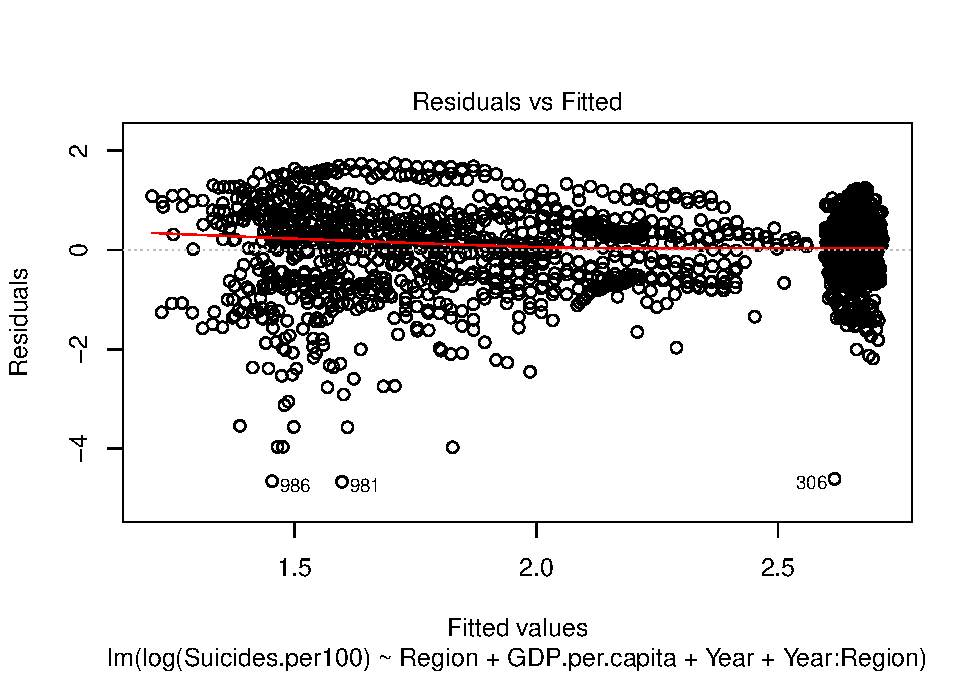
\includegraphics{An-Analysis-of-Suicide-Data_files/figure-latex/unnamed-chunk-10-1.pdf}

\begin{Shaded}
\begin{Highlighting}[]
\KeywordTok{plot}\NormalTok{(agg.fit6, }\DecValTok{2}\NormalTok{)}
\end{Highlighting}
\end{Shaded}

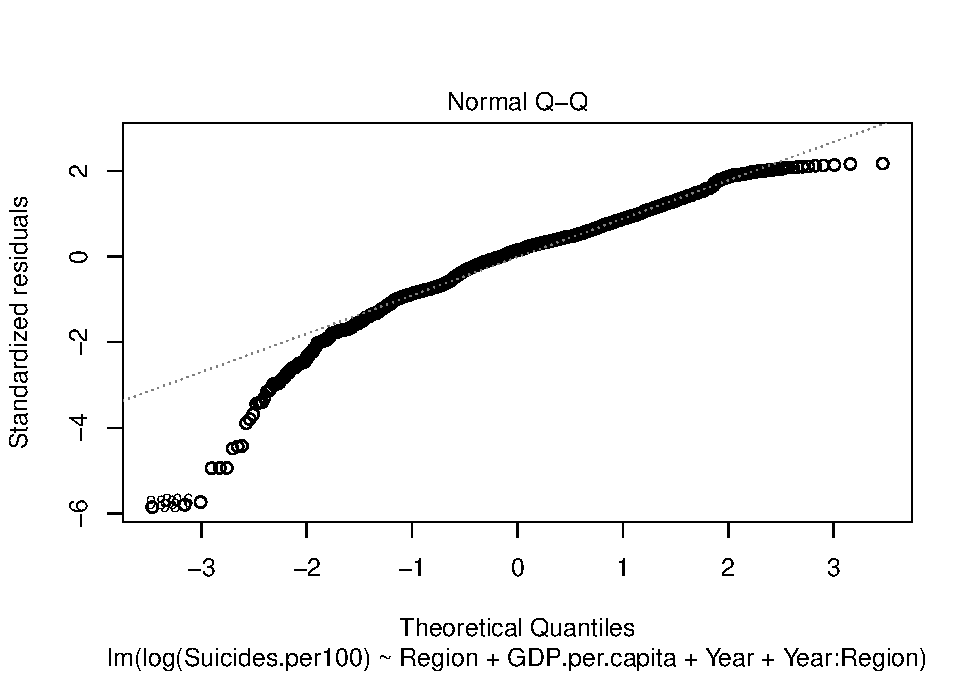
\includegraphics{An-Analysis-of-Suicide-Data_files/figure-latex/unnamed-chunk-10-2.pdf}

\begin{Shaded}
\begin{Highlighting}[]
\CommentTok{# since the normality assumption is broken, we should do bootstrapping for betas}
\NormalTok{n <-}\StringTok{ }\KeywordTok{nrow}\NormalTok{(agg.subset.rm)}
\NormalTok{i <-}\StringTok{ }\KeywordTok{sample}\NormalTok{(}\DecValTok{1}\OperatorTok{:}\NormalTok{n, n, }\DataTypeTok{replace=}\NormalTok{T)}
\KeywordTok{set.seed}\NormalTok{(}\DecValTok{12}\NormalTok{)}
\NormalTok{p.values <-}\StringTok{ }\KeywordTok{c}\NormalTok{()}
\NormalTok{confidence.lower <-}\StringTok{ }\KeywordTok{c}\NormalTok{()}
\NormalTok{confidence.upper <-}\StringTok{ }\KeywordTok{c}\NormalTok{()}
\NormalTok{beta.estimates <-}\StringTok{ }\KeywordTok{c}\NormalTok{()}

\ControlFlowTok{for}\NormalTok{ (index }\ControlFlowTok{in} \DecValTok{2}\OperatorTok{:}\DecValTok{17}\NormalTok{)\{}
\NormalTok{  beta1 <-}\StringTok{ }\ControlFlowTok{function}\NormalTok{(x,i) \{ }\KeywordTok{coef}\NormalTok{(}\KeywordTok{lm}\NormalTok{(}\KeywordTok{log}\NormalTok{(Suicides.per100) }\OperatorTok{~}\StringTok{ }\NormalTok{Region }\OperatorTok{+}\StringTok{ }\NormalTok{GDP.per.capita }\OperatorTok{+}\StringTok{ }\NormalTok{Year }\OperatorTok{+}\StringTok{ }\NormalTok{Year}\OperatorTok{:}\NormalTok{Region,}
                                   \DataTypeTok{data =}\NormalTok{ x,}
                                   \DataTypeTok{subset =}\NormalTok{ i))[index]\}}
  
  
\NormalTok{  res <-}\StringTok{ }\KeywordTok{boot}\NormalTok{(}\DataTypeTok{data =}\NormalTok{ agg.subset.rm,}
              \DataTypeTok{statistic =}\NormalTok{ beta1,}
              \DataTypeTok{R =} \DecValTok{1000}\NormalTok{)}
  
\NormalTok{  beta1.full <-}\StringTok{ }\KeywordTok{coef}\NormalTok{(}\KeywordTok{lm}\NormalTok{(}\KeywordTok{log}\NormalTok{(Suicides.per100) }\OperatorTok{~}\StringTok{ }\NormalTok{Region }\OperatorTok{+}\StringTok{ }\NormalTok{GDP.per.capita }\OperatorTok{+}\StringTok{ }\NormalTok{Year }\OperatorTok{+}\StringTok{ }\NormalTok{Year}\OperatorTok{:}\NormalTok{Region,}
                        \DataTypeTok{data=}\NormalTok{agg.subset.rm))[index]}
  
\NormalTok{  bias <-}\StringTok{ }\KeywordTok{mean}\NormalTok{(res}\OperatorTok{$}\NormalTok{t) }\OperatorTok{-}\StringTok{ }\NormalTok{beta1.full}
  
\NormalTok{  unbiased.est <-}\StringTok{ }\NormalTok{res}\OperatorTok{$}\NormalTok{t }\OperatorTok{-}\StringTok{ }\NormalTok{bias}
  
\NormalTok{  conf.low <-}\StringTok{ }\KeywordTok{quantile}\NormalTok{(unbiased.est, }\FloatTok{0.025}\NormalTok{)}
\NormalTok{  conf.up <-}\StringTok{ }\KeywordTok{quantile}\NormalTok{(unbiased.est, }\FloatTok{0.975}\NormalTok{)}
  
\NormalTok{  beta.H0 <-res}\OperatorTok{$}\NormalTok{t }\OperatorTok{-}\StringTok{ }\KeywordTok{mean}\NormalTok{(res}\OperatorTok{$}\NormalTok{t) }\OperatorTok{+}\StringTok{ }\NormalTok{bias}
  
\NormalTok{  p.val <-}\StringTok{ }\KeywordTok{mean}\NormalTok{(}\KeywordTok{abs}\NormalTok{(beta.H0) }\OperatorTok{>=}\StringTok{ }\KeywordTok{abs}\NormalTok{(beta1.full))}
  
\NormalTok{  beta.estimates <-}\StringTok{ }\KeywordTok{append}\NormalTok{(beta.estimates, beta1.full)}
\NormalTok{  p.values <-}\StringTok{ }\KeywordTok{append}\NormalTok{(p.values, p.val)}
\NormalTok{  confidence.lower <-}\StringTok{ }\KeywordTok{append}\NormalTok{(confidence.lower, conf.low)}
\NormalTok{  confidence.upper <-}\StringTok{ }\KeywordTok{append}\NormalTok{(confidence.upper, conf.up)}
  
  
\NormalTok{\}}

\NormalTok{boot.info6 <-}\StringTok{ }\KeywordTok{data.frame}\NormalTok{( beta.estimates, p.values)}
\KeywordTok{colnames}\NormalTok{(boot.info6) <-}\StringTok{ }\KeywordTok{c}\NormalTok{( }\StringTok{"Estimates"}\NormalTok{, }\StringTok{"P.value"}\NormalTok{)}
\CommentTok{# more accurate p-values}
\NormalTok{boot.info6}
\end{Highlighting}
\end{Shaded}

\begin{verbatim}
##                                Estimates P.value
## RegionAsia                 -1.960006e+01   0.720
## RegionCaribbean             5.179873e+00   0.915
## RegionCentral America      -7.140740e+01   0.140
## RegionEurope               -3.225869e+01   0.476
## RegionNorth America        -5.104462e+01   0.344
## RegionOceania              -4.169312e-01   0.995
## RegionSouth America        -9.102361e+01   0.065
## GDP.per.capita              3.217625e-07   0.698
## Year                       -2.095431e-02   0.359
## RegionAsia:Year             9.779824e-03   0.686
## RegionCaribbean:Year       -2.458825e-03   0.915
## RegionCentral America:Year  3.572629e-02   0.144
## RegionEurope:Year           1.669182e-02   0.508
## RegionNorth America:Year    2.581972e-02   0.308
## RegionOceania:Year          6.147560e-04   0.982
## RegionSouth America:Year    4.576185e-02   0.071
\end{verbatim}

\begin{Shaded}
\begin{Highlighting}[]
\CommentTok{# dataframe with old and new p-values}
\NormalTok{p.val.compare6 <-}\StringTok{ }\KeywordTok{data.frame}\NormalTok{(beta.estimates, agg.fit6.sum}\OperatorTok{$}\NormalTok{coefficients[}\DecValTok{2}\OperatorTok{:}\DecValTok{17}\NormalTok{,}\DecValTok{4}\NormalTok{], p.values)}
\KeywordTok{colnames}\NormalTok{(p.val.compare6) <-}\StringTok{ }\KeywordTok{c}\NormalTok{(}\StringTok{"estimates"}\NormalTok{, }\StringTok{"lm() p-values"}\NormalTok{, }\StringTok{"bootstrap p-values"}\NormalTok{)}

\NormalTok{p.val.compare6}
\end{Highlighting}
\end{Shaded}

\begin{verbatim}
##                                estimates lm() p-values bootstrap p-values
## RegionAsia                 -1.960006e+01   0.577600269              0.720
## RegionCaribbean             5.179873e+00   0.873414740              0.915
## RegionCentral America      -7.140740e+01   0.048708886              0.140
## RegionEurope               -3.225869e+01   0.304107612              0.476
## RegionNorth America        -5.104462e+01   0.196455570              0.344
## RegionOceania              -4.169312e-01   0.991905022              0.995
## RegionSouth America        -9.102361e+01   0.007121525              0.065
## GDP.per.capita              3.217625e-07   0.768255485              0.698
## Year                       -2.095431e-02   0.166861597              0.359
## RegionAsia:Year             9.779824e-03   0.577571880              0.686
## RegionCaribbean:Year       -2.458825e-03   0.879486672              0.915
## RegionCentral America:Year  3.572629e-02   0.048057715              0.144
## RegionEurope:Year           1.669182e-02   0.286395247              0.508
## RegionNorth America:Year    2.581972e-02   0.190446185              0.308
## RegionOceania:Year          6.147560e-04   0.976089708              0.982
## RegionSouth America:Year    4.576185e-02   0.006687764              0.071
\end{verbatim}

\begin{Shaded}
\begin{Highlighting}[]
\KeywordTok{AIC}\NormalTok{(agg.fit6)}
\end{Highlighting}
\end{Shaded}

\begin{verbatim}
## [1] 4585.991
\end{verbatim}

\begin{Shaded}
\begin{Highlighting}[]
\CommentTok{## Interaction between Year/Region and GDP/Region}
\CommentTok{## Interaction between GDP and Region}
\NormalTok{agg.fit7 <-}\StringTok{ }\KeywordTok{lm}\NormalTok{(}\KeywordTok{log}\NormalTok{(Suicides.per100) }\OperatorTok{~}\StringTok{ }\NormalTok{Region }\OperatorTok{+}\StringTok{ }\NormalTok{GDP.per.capita }\OperatorTok{+}\StringTok{ }\NormalTok{Year }\OperatorTok{+}\StringTok{ }\NormalTok{GDP.per.capita}\OperatorTok{:}\NormalTok{Region }\OperatorTok{+}\StringTok{ }\NormalTok{Year}\OperatorTok{:}\NormalTok{Region, }\DataTypeTok{data =}\NormalTok{ agg.subset.rm)}
\NormalTok{agg.fit7.sum <-}\StringTok{ }\KeywordTok{summary}\NormalTok{(agg.fit7)}

\CommentTok{# heteroskedasticity is mosly fixed, but residuals are not normally distributed}
\KeywordTok{plot}\NormalTok{(agg.fit7, }\DecValTok{1}\NormalTok{)}
\end{Highlighting}
\end{Shaded}

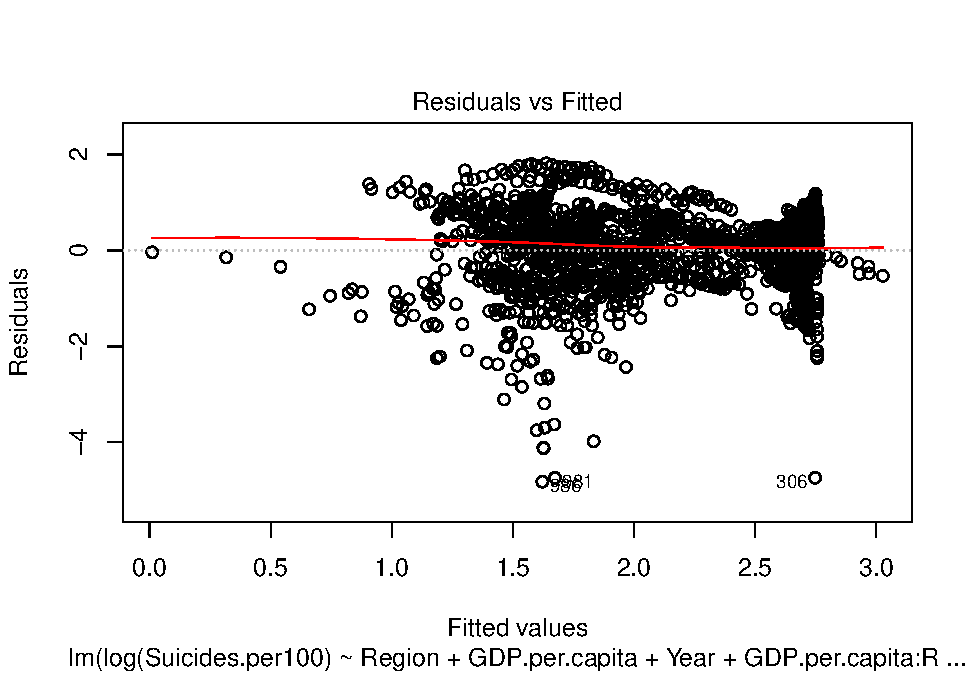
\includegraphics{An-Analysis-of-Suicide-Data_files/figure-latex/unnamed-chunk-11-1.pdf}

\begin{Shaded}
\begin{Highlighting}[]
\KeywordTok{plot}\NormalTok{(agg.fit7, }\DecValTok{2}\NormalTok{)}
\end{Highlighting}
\end{Shaded}

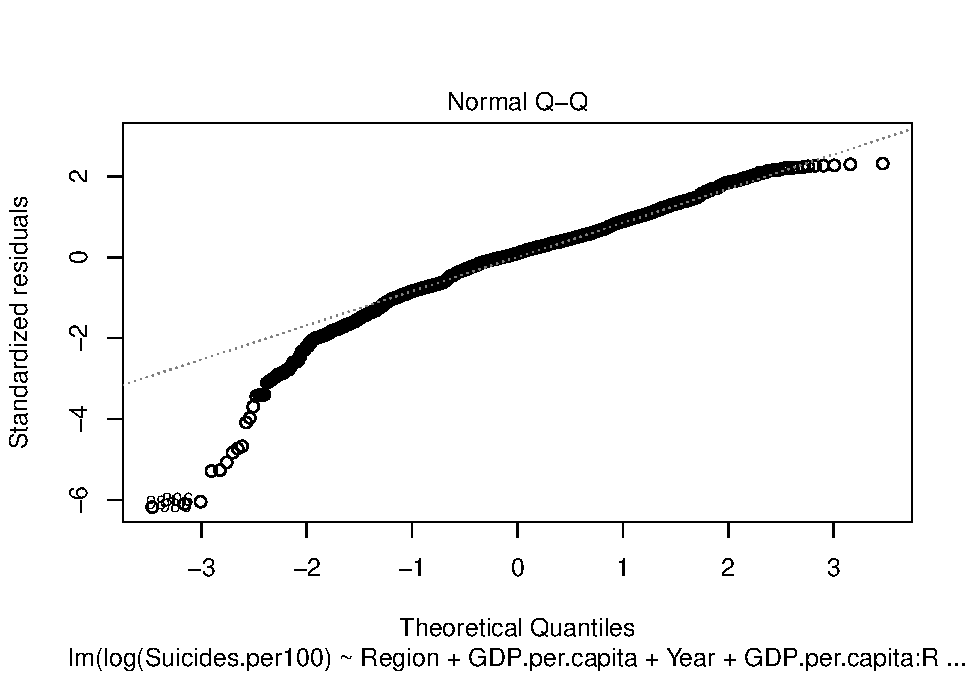
\includegraphics{An-Analysis-of-Suicide-Data_files/figure-latex/unnamed-chunk-11-2.pdf}

\begin{Shaded}
\begin{Highlighting}[]
\CommentTok{# since the normality assumption is broken, we should do bootstrapping for betas}
\NormalTok{n <-}\StringTok{ }\KeywordTok{nrow}\NormalTok{(agg.subset.rm)}
\NormalTok{i <-}\StringTok{ }\KeywordTok{sample}\NormalTok{(}\DecValTok{1}\OperatorTok{:}\NormalTok{n, n, }\DataTypeTok{replace=}\NormalTok{T)}
\KeywordTok{set.seed}\NormalTok{(}\DecValTok{12}\NormalTok{)}
\NormalTok{p.values <-}\StringTok{ }\KeywordTok{c}\NormalTok{()}
\NormalTok{confidence.lower <-}\StringTok{ }\KeywordTok{c}\NormalTok{()}
\NormalTok{confidence.upper <-}\StringTok{ }\KeywordTok{c}\NormalTok{()}
\NormalTok{beta.estimates <-}\StringTok{ }\KeywordTok{c}\NormalTok{()}

\ControlFlowTok{for}\NormalTok{ (index }\ControlFlowTok{in} \DecValTok{2}\OperatorTok{:}\DecValTok{24}\NormalTok{)\{}
\NormalTok{  beta1 <-}\StringTok{ }\ControlFlowTok{function}\NormalTok{(x,i) \{ }\KeywordTok{coef}\NormalTok{(}\KeywordTok{lm}\NormalTok{(}\KeywordTok{log}\NormalTok{(Suicides.per100) }\OperatorTok{~}\StringTok{ }\NormalTok{Region }\OperatorTok{+}\StringTok{ }\NormalTok{GDP.per.capita }\OperatorTok{+}\StringTok{ }\NormalTok{Year }\OperatorTok{+}\StringTok{ }\NormalTok{GDP.per.capita}\OperatorTok{:}\NormalTok{Region}\OperatorTok{+}\StringTok{ }\NormalTok{Year}\OperatorTok{:}\NormalTok{Region,}
                                   \DataTypeTok{data =}\NormalTok{ x,}
                                   \DataTypeTok{subset =}\NormalTok{ i))[index]\}}
  
  
\NormalTok{  res <-}\StringTok{ }\KeywordTok{boot}\NormalTok{(}\DataTypeTok{data =}\NormalTok{ agg.subset.rm,}
              \DataTypeTok{statistic =}\NormalTok{ beta1,}
              \DataTypeTok{R =} \DecValTok{1000}\NormalTok{)}
  
\NormalTok{  beta1.full <-}\StringTok{ }\KeywordTok{coef}\NormalTok{(}\KeywordTok{lm}\NormalTok{(}\KeywordTok{log}\NormalTok{(Suicides.per100) }\OperatorTok{~}\StringTok{ }\NormalTok{Region }\OperatorTok{+}\StringTok{ }\NormalTok{GDP.per.capita }\OperatorTok{+}\StringTok{ }\NormalTok{Year }\OperatorTok{+}\StringTok{ }\NormalTok{GDP.per.capita}\OperatorTok{:}\NormalTok{Region }\OperatorTok{+}\StringTok{ }\NormalTok{Year}\OperatorTok{:}\NormalTok{Region,}
                        \DataTypeTok{data=}\NormalTok{agg.subset.rm))[index]}
  
\NormalTok{  bias <-}\StringTok{ }\KeywordTok{mean}\NormalTok{(res}\OperatorTok{$}\NormalTok{t) }\OperatorTok{-}\StringTok{ }\NormalTok{beta1.full}
  
\NormalTok{  unbiased.est <-}\StringTok{ }\NormalTok{res}\OperatorTok{$}\NormalTok{t }\OperatorTok{-}\StringTok{ }\NormalTok{bias}
  
\NormalTok{  conf.low <-}\StringTok{ }\KeywordTok{quantile}\NormalTok{(unbiased.est, }\FloatTok{0.025}\NormalTok{)}
\NormalTok{  conf.up <-}\StringTok{ }\KeywordTok{quantile}\NormalTok{(unbiased.est, }\FloatTok{0.975}\NormalTok{)}
  
\NormalTok{  beta.H0 <-res}\OperatorTok{$}\NormalTok{t }\OperatorTok{-}\StringTok{ }\KeywordTok{mean}\NormalTok{(res}\OperatorTok{$}\NormalTok{t) }\OperatorTok{+}\StringTok{ }\NormalTok{bias}
  
\NormalTok{  p.val <-}\StringTok{ }\KeywordTok{mean}\NormalTok{(}\KeywordTok{abs}\NormalTok{(beta.H0) }\OperatorTok{>=}\StringTok{ }\KeywordTok{abs}\NormalTok{(beta1.full))}
  
\NormalTok{  beta.estimates <-}\StringTok{ }\KeywordTok{append}\NormalTok{(beta.estimates, beta1.full)}
\NormalTok{  p.values <-}\StringTok{ }\KeywordTok{append}\NormalTok{(p.values, p.val)}
\NormalTok{  confidence.lower <-}\StringTok{ }\KeywordTok{append}\NormalTok{(confidence.lower, conf.low)}
\NormalTok{  confidence.upper <-}\StringTok{ }\KeywordTok{append}\NormalTok{(confidence.upper, conf.up)}
  
  
\NormalTok{\}}

\NormalTok{boot.info7 <-}\StringTok{ }\KeywordTok{data.frame}\NormalTok{( beta.estimates, p.values)}
\KeywordTok{colnames}\NormalTok{(boot.info7) <-}\StringTok{ }\KeywordTok{c}\NormalTok{( }\StringTok{"Estimates"}\NormalTok{, }\StringTok{"P.value"}\NormalTok{)}
\CommentTok{# more accurate p-values}
\NormalTok{boot.info7}
\end{Highlighting}
\end{Shaded}

\begin{verbatim}
##                                          Estimates P.value
## RegionAsia                           -2.318194e+02   0.000
## RegionCaribbean                      -1.771861e+02   0.002
## RegionCentral America                -2.649234e+02   0.000
## RegionEurope                         -2.342437e+02   0.001
## RegionNorth America                  -1.828136e+02   0.003
## RegionOceania                        -1.099626e+02   0.045
## RegionSouth America                  -2.749275e+02   0.000
## GDP.per.capita                        2.432516e-04   0.000
## Year                                 -1.178336e-01   0.000
## RegionAsia:GDP.per.capita            -2.596697e-04   0.001
## RegionCaribbean:GDP.per.capita       -2.374882e-04   0.000
## RegionCentral America:GDP.per.capita -2.455955e-04   0.000
## RegionEurope:GDP.per.capita          -2.472868e-04   0.000
## RegionNorth America:GDP.per.capita   -2.133317e-04   0.000
## RegionOceania:GDP.per.capita         -2.163836e-04   0.000
## RegionSouth America:GDP.per.capita   -2.301690e-04   0.000
## RegionAsia:Year                       1.166466e-01   0.001
## RegionCaribbean:Year                  8.934979e-02   0.004
## RegionCentral America:Year            1.331477e-01   0.000
## RegionEurope:Year                     1.183930e-01   0.000
## RegionNorth America:Year              9.198386e-02   0.004
## RegionOceania:Year                    5.578112e-02   0.045
## RegionSouth America:Year              1.383423e-01   0.000
\end{verbatim}

\begin{Shaded}
\begin{Highlighting}[]
\CommentTok{# dataframe with old and new p-values}
\NormalTok{p.val.compare7 <-}\StringTok{ }\KeywordTok{data.frame}\NormalTok{(beta.estimates, agg.fit7.sum}\OperatorTok{$}\NormalTok{coefficients[}\DecValTok{2}\OperatorTok{:}\DecValTok{24}\NormalTok{,}\DecValTok{4}\NormalTok{], p.values)}
\KeywordTok{colnames}\NormalTok{(p.val.compare7) <-}\StringTok{ }\KeywordTok{c}\NormalTok{(}\StringTok{"estimates"}\NormalTok{, }\StringTok{"lm() p-values"}\NormalTok{, }\StringTok{"bootstrap p-values"}\NormalTok{)}

\NormalTok{p.val.compare7}
\end{Highlighting}
\end{Shaded}

\begin{verbatim}
##                                          estimates lm() p-values
## RegionAsia                           -2.318194e+02  2.308233e-06
## RegionCaribbean                      -1.771861e+02  1.457249e-04
## RegionCentral America                -2.649234e+02  1.682285e-07
## RegionEurope                         -2.342437e+02  3.298471e-07
## RegionNorth America                  -1.828136e+02  5.226782e-04
## RegionOceania                        -1.099626e+02  4.988077e-02
## RegionSouth America                  -2.749275e+02  1.685879e-08
## GDP.per.capita                        2.432516e-04  1.445883e-08
## Year                                 -1.178336e-01  1.952312e-07
## RegionAsia:GDP.per.capita            -2.596697e-04  2.388519e-09
## RegionCaribbean:GDP.per.capita       -2.374882e-04  3.245908e-08
## RegionCentral America:GDP.per.capita -2.455955e-04  3.085616e-06
## RegionEurope:GDP.per.capita          -2.472868e-04  8.491497e-09
## RegionNorth America:GDP.per.capita   -2.133317e-04  8.140411e-07
## RegionOceania:GDP.per.capita         -2.163836e-04  5.976810e-07
## RegionSouth America:GDP.per.capita   -2.301690e-04  5.444470e-07
## RegionAsia:Year                       1.166466e-01  2.112265e-06
## RegionCaribbean:Year                  8.934979e-02  1.330144e-04
## RegionCentral America:Year            1.331477e-01  1.560563e-07
## RegionEurope:Year                     1.183930e-01  2.650724e-07
## RegionNorth America:Year              9.198386e-02  4.972062e-04
## RegionOceania:Year                    5.578112e-02  4.717508e-02
## RegionSouth America:Year              1.383423e-01  1.493343e-08
##                                      bootstrap p-values
## RegionAsia                                        0.000
## RegionCaribbean                                   0.002
## RegionCentral America                             0.000
## RegionEurope                                      0.001
## RegionNorth America                               0.003
## RegionOceania                                     0.045
## RegionSouth America                               0.000
## GDP.per.capita                                    0.000
## Year                                              0.000
## RegionAsia:GDP.per.capita                         0.001
## RegionCaribbean:GDP.per.capita                    0.000
## RegionCentral America:GDP.per.capita              0.000
## RegionEurope:GDP.per.capita                       0.000
## RegionNorth America:GDP.per.capita                0.000
## RegionOceania:GDP.per.capita                      0.000
## RegionSouth America:GDP.per.capita                0.000
## RegionAsia:Year                                   0.001
## RegionCaribbean:Year                              0.004
## RegionCentral America:Year                        0.000
## RegionEurope:Year                                 0.000
## RegionNorth America:Year                          0.004
## RegionOceania:Year                                0.045
## RegionSouth America:Year                          0.000
\end{verbatim}

\begin{Shaded}
\begin{Highlighting}[]
\KeywordTok{AIC}\NormalTok{(agg.fit7)}
\end{Highlighting}
\end{Shaded}

\begin{verbatim}
## [1] 4500.869
\end{verbatim}

This model has a much better AIC and the R\^{}2 increased quite a bit,
but it seems to be getting into the realm of overfitting. Considering
this, I am going to remain more conservative and use the simpler model
with the interaction between GDP and Region. This will be easier to
interpret and can be quite a bit insightful, while not being overfit to
the data.

\hypertarget{final-model-for-aggregate-data}{%
\subsection{Final Model for Aggregate
Data}\label{final-model-for-aggregate-data}}

\begin{Shaded}
\begin{Highlighting}[]
\CommentTok{## interaction between GDP and Region}
\NormalTok{agg.fit5.sum}
\end{Highlighting}
\end{Shaded}

\begin{verbatim}
## 
## Call:
## lm(formula = log(Suicides.per100) ~ Region + GDP.per.capita + 
##     Year + GDP.per.capita:Region, data = agg.subset.rm)
## 
## Residuals:
##     Min      1Q  Median      3Q     Max 
## -4.7957 -0.4116  0.0900  0.4588  1.8294 
## 
## Coefficients:
##                                        Estimate Std. Error t value
## (Intercept)                           1.622e+01  5.612e+00   2.890
## RegionAsia                            8.438e-01  2.560e-01   3.297
## RegionCaribbean                       8.652e-01  2.409e-01   3.592
## RegionCentral America                 6.916e-01  2.687e-01   2.574
## RegionEurope                          1.925e+00  2.387e-01   8.067
## RegionNorth America                   5.894e-01  2.908e-01   2.027
## RegionOceania                         1.166e+00  2.795e-01   4.171
## RegionSouth America                   1.038e+00  2.514e-01   4.130
## GDP.per.capita                        8.567e-05  2.872e-05   2.983
## Year                                 -7.691e-03  2.811e-03  -2.735
## RegionAsia:GDP.per.capita            -1.001e-04  2.932e-05  -3.413
## RegionCaribbean:GDP.per.capita       -8.246e-05  2.875e-05  -2.868
## RegionCentral America:GDP.per.capita -5.473e-05  3.854e-05  -1.420
## RegionEurope:GDP.per.capita          -8.876e-05  2.871e-05  -3.092
## RegionNorth America:GDP.per.capita   -5.906e-05  2.913e-05  -2.027
## RegionOceania:GDP.per.capita         -7.108e-05  2.911e-05  -2.442
## RegionSouth America:GDP.per.capita   -4.156e-05  3.139e-05  -1.324
##                                      Pr(>|t|)    
## (Intercept)                          0.003897 ** 
## RegionAsia                           0.000996 ***
## RegionCaribbean                      0.000337 ***
## RegionCentral America                0.010135 *  
## RegionEurope                         1.27e-15 ***
## RegionNorth America                  0.042823 *  
## RegionOceania                        3.17e-05 ***
## RegionSouth America                  3.78e-05 ***
## GDP.per.capita                       0.002895 ** 
## Year                                 0.006289 ** 
## RegionAsia:GDP.per.capita            0.000656 ***
## RegionCaribbean:GDP.per.capita       0.004177 ** 
## RegionCentral America:GDP.per.capita 0.155772    
## RegionEurope:GDP.per.capita          0.002018 ** 
## RegionNorth America:GDP.per.capita   0.042770 *  
## RegionOceania:GDP.per.capita         0.014685 *  
## RegionSouth America:GDP.per.capita   0.185628    
## ---
## Signif. codes:  0 '***' 0.001 '**' 0.01 '*' 0.05 '.' 0.1 ' ' 1
## 
## Residual standard error: 0.7989 on 1881 degrees of freedom
##   (116 observations deleted due to missingness)
## Multiple R-squared:  0.2789, Adjusted R-squared:  0.2728 
## F-statistic: 45.47 on 16 and 1881 DF,  p-value: < 2.2e-16
\end{verbatim}

\begin{Shaded}
\begin{Highlighting}[]
\NormalTok{p.val.compare5}
\end{Highlighting}
\end{Shaded}

\begin{verbatim}
##                                          estimates lm() p-values
## RegionAsia                            8.438418e-01  9.960212e-04
## RegionCaribbean                       8.652377e-01  3.367675e-04
## RegionCentral America                 6.915980e-01  1.013530e-02
## RegionEurope                          1.925448e+00  1.271913e-15
## RegionNorth America                   5.893887e-01  4.282314e-02
## RegionOceania                         1.165874e+00  3.174611e-05
## RegionSouth America                   1.038377e+00  3.782845e-05
## GDP.per.capita                        8.567196e-05  2.894590e-03
## Year                                 -7.690527e-03  6.288511e-03
## RegionAsia:GDP.per.capita            -1.000537e-04  6.560624e-04
## RegionCaribbean:GDP.per.capita       -8.246098e-05  4.176855e-03
## RegionCentral America:GDP.per.capita -5.472676e-05  1.557719e-01
## RegionEurope:GDP.per.capita          -8.875707e-05  2.018367e-03
## RegionNorth America:GDP.per.capita   -5.905528e-05  4.277041e-02
## RegionOceania:GDP.per.capita         -7.108485e-05  1.468454e-02
## RegionSouth America:GDP.per.capita   -4.156215e-05  1.856278e-01
##                                      bootstrap p-values
## RegionAsia                                        0.051
## RegionCaribbean                                   0.036
## RegionCentral America                             0.089
## RegionEurope                                      0.000
## RegionNorth America                               0.166
## RegionOceania                                     0.005
## RegionSouth America                               0.013
## GDP.per.capita                                    0.018
## Year                                              0.002
## RegionAsia:GDP.per.capita                         0.015
## RegionCaribbean:GDP.per.capita                    0.040
## RegionCentral America:GDP.per.capita              0.185
## RegionEurope:GDP.per.capita                       0.010
## RegionNorth America:GDP.per.capita                0.115
## RegionOceania:GDP.per.capita                      0.068
## RegionSouth America:GDP.per.capita                0.279
\end{verbatim}

\begin{Shaded}
\begin{Highlighting}[]
\KeywordTok{AIC}\NormalTok{(agg.fit5)}
\end{Highlighting}
\end{Shaded}

\begin{verbatim}
## [1] 4553.103
\end{verbatim}

\hypertarget{model-interpretation-and-visualization-1}{%
\subsection{Model Interpretation and
Visualization}\label{model-interpretation-and-visualization-1}}

\begin{Shaded}
\begin{Highlighting}[]
\CommentTok{# interpretation of ceofficients}
\KeywordTok{kable}\NormalTok{(}\KeywordTok{coef}\NormalTok{(agg.fit5.sum))}
\end{Highlighting}
\end{Shaded}

\begin{longtable}[]{@{}lrrrr@{}}
\toprule
& Estimate & Std. Error & t value &
Pr(\textgreater\textbar t\textbar)\tabularnewline
\midrule
\endhead
(Intercept) & 16.2184112 & 5.6120514 & 2.889926 &
0.0038975\tabularnewline
RegionAsia & 0.8438418 & 0.2559553 & 3.296833 & 0.0009960\tabularnewline
RegionCaribbean & 0.8652377 & 0.2408889 & 3.591853 &
0.0003368\tabularnewline
RegionCentral America & 0.6915980 & 0.2687088 & 2.573782 &
0.0101353\tabularnewline
RegionEurope & 1.9254483 & 0.2386869 & 8.066837 &
0.0000000\tabularnewline
RegionNorth America & 0.5893887 & 0.2907969 & 2.026805 &
0.0428231\tabularnewline
RegionOceania & 1.1658739 & 0.2795383 & 4.170712 &
0.0000317\tabularnewline
RegionSouth America & 1.0383767 & 0.2514093 & 4.130224 &
0.0000378\tabularnewline
GDP.per.capita & 0.0000857 & 0.0000287 & 2.982629 &
0.0028946\tabularnewline
Year & -0.0076905 & 0.0028115 & -2.735423 & 0.0062885\tabularnewline
RegionAsia:GDP.per.capita & -0.0001001 & 0.0000293 & -3.413031 &
0.0006561\tabularnewline
RegionCaribbean:GDP.per.capita & -0.0000825 & 0.0000288 & -2.867995 &
0.0041769\tabularnewline
RegionCentral America:GDP.per.capita & -0.0000547 & 0.0000385 &
-1.420005 & 0.1557719\tabularnewline
RegionEurope:GDP.per.capita & -0.0000888 & 0.0000287 & -3.091844 &
0.0020184\tabularnewline
RegionNorth America:GDP.per.capita & -0.0000591 & 0.0000291 & -2.027321
& 0.0427704\tabularnewline
RegionOceania:GDP.per.capita & -0.0000711 & 0.0000291 & -2.442324 &
0.0146845\tabularnewline
RegionSouth America:GDP.per.capita & -0.0000416 & 0.0000314 & -1.324109
& 0.1856278\tabularnewline
\bottomrule
\end{longtable}

\begin{Shaded}
\begin{Highlighting}[]
\CommentTok{# visualizations of suicides with region and GDP changing, while year is held constant at 2015}
\NormalTok{year.pred <-}\StringTok{ }\DecValTok{2015}
\NormalTok{region.pred <-}\StringTok{ }\KeywordTok{levels}\NormalTok{(agg.subset.rm}\OperatorTok{$}\NormalTok{Region)}
\NormalTok{gdp.seq <-}\StringTok{ }\KeywordTok{seq}\NormalTok{(}\KeywordTok{min}\NormalTok{(aggregate.suicides}\OperatorTok{$}\NormalTok{GDP.per.capita), }\KeywordTok{max}\NormalTok{(aggregate.suicides}\OperatorTok{$}\NormalTok{GDP.per.capita), }\DataTypeTok{length.out =} \DecValTok{1000}\NormalTok{)}

\NormalTok{expand.grid.demo1 <-}\StringTok{ }\KeywordTok{expand.grid}\NormalTok{(region.pred, gdp.seq, year.pred)}
\KeywordTok{colnames}\NormalTok{(expand.grid.demo1) <-}\StringTok{ }\KeywordTok{c}\NormalTok{(}\StringTok{"Region"}\NormalTok{, }\StringTok{"GDP.per.capita"}\NormalTok{, }\StringTok{"Year"}\NormalTok{)}

\NormalTok{demo.expand.pred1 <-}\StringTok{ }\KeywordTok{predict}\NormalTok{(agg.fit5, }\DataTypeTok{newdata =}\NormalTok{ expand.grid.demo1)}

\NormalTok{demo.pred.data1 <-}\StringTok{ }\KeywordTok{cbind}\NormalTok{(expand.grid.demo1, demo.expand.pred1)}
\KeywordTok{colnames}\NormalTok{(demo.pred.data1) <-}\StringTok{ }\KeywordTok{c}\NormalTok{(}\StringTok{"Region"}\NormalTok{, }\StringTok{"GDP.per.capita"}\NormalTok{, }\StringTok{"Year"}\NormalTok{, }\StringTok{"Suicides.per100"}\NormalTok{)}

\KeywordTok{ggplot}\NormalTok{(demo.pred.data1, }\KeywordTok{aes}\NormalTok{(}\DataTypeTok{x =}\NormalTok{ GDP.per.capita, }\DataTypeTok{y =} \KeywordTok{exp}\NormalTok{(Suicides.per100), }\DataTypeTok{color =}\NormalTok{ Region)) }\OperatorTok{+}\StringTok{ }
\StringTok{  }\KeywordTok{geom_line}\NormalTok{() }\OperatorTok{+}\StringTok{ }
\StringTok{  }\KeywordTok{labs}\NormalTok{(}\DataTypeTok{x =} \StringTok{"GDP per capita"}\NormalTok{, }\DataTypeTok{y =} \StringTok{"Predicted Suicides per 100k"}\NormalTok{, }\DataTypeTok{title =} \StringTok{"Predicted Suicides by Region"}\NormalTok{) }\OperatorTok{+}
\StringTok{  }\KeywordTok{lims}\NormalTok{(}\DataTypeTok{x =} \KeywordTok{c}\NormalTok{(}\DecValTok{0}\NormalTok{, }\DecValTok{100000}\NormalTok{), }\DataTypeTok{y =} \KeywordTok{c}\NormalTok{(}\DecValTok{0}\NormalTok{, }\DecValTok{50}\NormalTok{))}
\end{Highlighting}
\end{Shaded}

\begin{verbatim}
## Warning: Removed 2747 rows containing missing values (geom_path).
\end{verbatim}

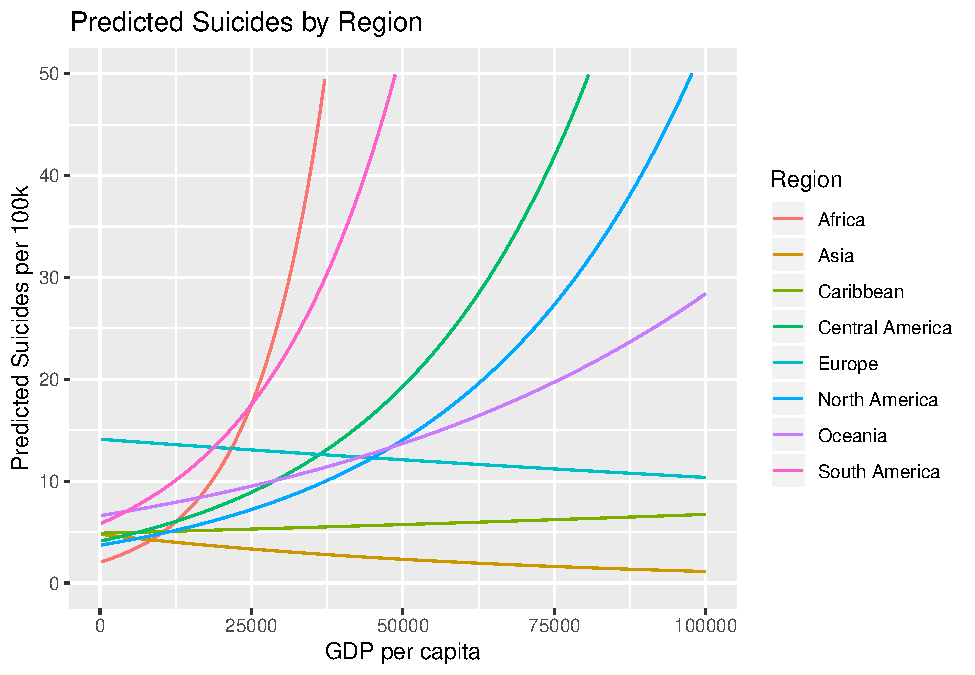
\includegraphics{An-Analysis-of-Suicide-Data_files/figure-latex/unnamed-chunk-13-1.pdf}

\begin{Shaded}
\begin{Highlighting}[]
\CommentTok{##################################################################################}
\CommentTok{# 3d plot with year and GDP changing, region held constant at North America}
\NormalTok{year.pred <-}\StringTok{ }\KeywordTok{seq}\NormalTok{(}\DecValTok{1990}\NormalTok{, }\DecValTok{2016}\NormalTok{,}\DecValTok{1}\NormalTok{)}
\NormalTok{region.pred <-}\StringTok{ "North America"}
\NormalTok{gdp.seq <-}\StringTok{ }\KeywordTok{seq}\NormalTok{(}\KeywordTok{min}\NormalTok{(aggregate.suicides}\OperatorTok{$}\NormalTok{GDP.per.capita), }\KeywordTok{max}\NormalTok{(aggregate.suicides}\OperatorTok{$}\NormalTok{GDP.per.capita), }\DataTypeTok{length.out =} \DecValTok{1000}\NormalTok{)}

\NormalTok{expand.grid.demo3 <-}\StringTok{ }\KeywordTok{expand.grid}\NormalTok{(region.pred, gdp.seq, year.pred)}
\KeywordTok{colnames}\NormalTok{(expand.grid.demo3) <-}\StringTok{ }\KeywordTok{c}\NormalTok{(}\StringTok{"Region"}\NormalTok{, }\StringTok{"GDP.per.capita"}\NormalTok{, }\StringTok{"Year"}\NormalTok{)}

\NormalTok{demo.expand.pred3 <-}\StringTok{ }\KeywordTok{predict}\NormalTok{(agg.fit5, }\DataTypeTok{newdata =}\NormalTok{ expand.grid.demo3)}

\NormalTok{demo.pred.data3 <-}\StringTok{ }\KeywordTok{cbind}\NormalTok{(expand.grid.demo3, demo.expand.pred3)}
\KeywordTok{colnames}\NormalTok{(demo.pred.data3) <-}\StringTok{ }\KeywordTok{c}\NormalTok{(}\StringTok{"Region"}\NormalTok{, }\StringTok{"GDP.per.capita"}\NormalTok{, }\StringTok{"Year"}\NormalTok{, }\StringTok{"Suicides.per100"}\NormalTok{)}
\NormalTok{x=demo.pred.data3}\OperatorTok{$}\NormalTok{GDP.per.capita}
\NormalTok{y=demo.pred.data3}\OperatorTok{$}\NormalTok{Year}
\NormalTok{z=demo.pred.data3}\OperatorTok{$}\NormalTok{Suicides.per100}

\CommentTok{#persp(x, y, z., theta = 50, phi = 0, }
      \CommentTok{#col = "yellow", expand = 0.5, xlab = "GDP per capita", ylab = "Year", zlab = "Suicides per 100k")}
\CommentTok{#################################################################################}
\end{Highlighting}
\end{Shaded}

Interpretation of GDP:

Interpretation of Region:

\hypertarget{comparison-of-trends-of-suicides-over-the-years-by-region}{%
\subsection{Comparison of trends of suicides over the years by
region}\label{comparison-of-trends-of-suicides-over-the-years-by-region}}

\begin{Shaded}
\begin{Highlighting}[]
\NormalTok{agg.fit8 <-}\StringTok{ }\KeywordTok{lm}\NormalTok{(}\KeywordTok{log}\NormalTok{(Suicides.per100) }\OperatorTok{~}\StringTok{ }\NormalTok{Region }\OperatorTok{+}\StringTok{ }\NormalTok{Year }\OperatorTok{+}\StringTok{ }\NormalTok{Year}\OperatorTok{:}\NormalTok{Region, }\DataTypeTok{data =}\NormalTok{ agg.subset.rm)}
\NormalTok{agg.fit8.sum <-}\StringTok{ }\KeywordTok{summary}\NormalTok{(agg.fit8)}

\CommentTok{# visualizations of suicides with region and year changing}
\NormalTok{year.pred <-}\StringTok{ }\KeywordTok{seq}\NormalTok{(}\DecValTok{1990}\NormalTok{, }\DecValTok{2016}\NormalTok{, }\DecValTok{1}\NormalTok{)}
\NormalTok{region.pred <-}\StringTok{ }\KeywordTok{levels}\NormalTok{(aggregate.suicides}\OperatorTok{$}\NormalTok{Region)}

\NormalTok{expand.grid.demo2 <-}\StringTok{ }\KeywordTok{expand.grid}\NormalTok{(region.pred, year.pred)}
\KeywordTok{colnames}\NormalTok{(expand.grid.demo2) <-}\StringTok{ }\KeywordTok{c}\NormalTok{(}\StringTok{"Region"}\NormalTok{, }\StringTok{"Year"}\NormalTok{)}

\NormalTok{demo.expand.pred2 <-}\StringTok{ }\KeywordTok{predict}\NormalTok{(agg.fit8, }\DataTypeTok{newdata =}\NormalTok{ expand.grid.demo2)}

\NormalTok{demo.pred.data2 <-}\StringTok{ }\KeywordTok{cbind}\NormalTok{(expand.grid.demo2, demo.expand.pred2)}
\KeywordTok{colnames}\NormalTok{(demo.pred.data2) <-}\StringTok{ }\KeywordTok{c}\NormalTok{(}\StringTok{"Region"}\NormalTok{, }\StringTok{"Year"}\NormalTok{, }\StringTok{"Suicides.per100"}\NormalTok{)}

\KeywordTok{ggplot}\NormalTok{(demo.pred.data2, }\KeywordTok{aes}\NormalTok{(}\DataTypeTok{x =}\NormalTok{ Year, }\DataTypeTok{y =} \KeywordTok{exp}\NormalTok{(Suicides.per100) , }\DataTypeTok{color =}\NormalTok{ Region)) }\OperatorTok{+}\StringTok{ }
\StringTok{  }\KeywordTok{geom_line}\NormalTok{() }\OperatorTok{+}\StringTok{ }
\StringTok{  }\KeywordTok{labs}\NormalTok{(}\DataTypeTok{x =} \StringTok{"Year"}\NormalTok{, }\DataTypeTok{y =} \StringTok{"Predicted Suicides per 100k"}\NormalTok{, }\DataTypeTok{title =} \StringTok{"Trends of Suicides by Region and Year"}\NormalTok{) }\OperatorTok{+}
\StringTok{  }\KeywordTok{lims}\NormalTok{(}\DataTypeTok{x =} \KeywordTok{c}\NormalTok{(}\DecValTok{1990}\NormalTok{, }\DecValTok{2016}\NormalTok{))}
\end{Highlighting}
\end{Shaded}

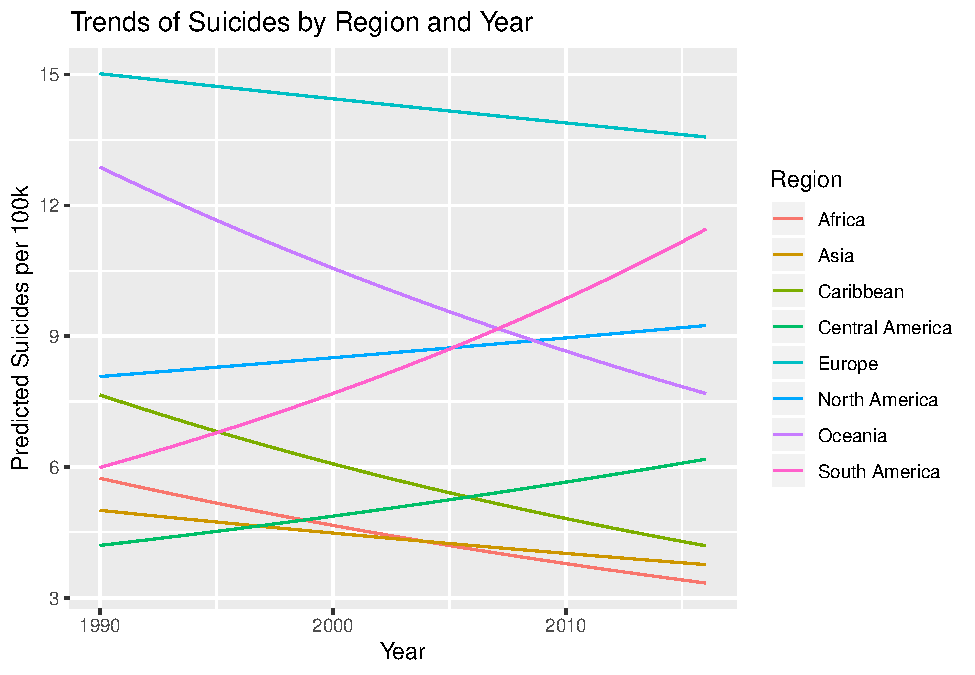
\includegraphics{An-Analysis-of-Suicide-Data_files/figure-latex/unnamed-chunk-14-1.pdf}

\hypertarget{other}{%
\section{Other}\label{other}}

\begin{Shaded}
\begin{Highlighting}[]
\CommentTok{# What if I did the same thing above but with a log(y+1) transformation without removing the zeros?}
\NormalTok{agg.fit9 <-}\StringTok{ }\KeywordTok{lm}\NormalTok{(}\KeywordTok{log}\NormalTok{(Suicides.per100 }\OperatorTok{+}\StringTok{ }\DecValTok{1}\NormalTok{) }\OperatorTok{~}\StringTok{ }\NormalTok{Region }\OperatorTok{+}\StringTok{ }\NormalTok{GDP.per.capita }\OperatorTok{+}\StringTok{ }\NormalTok{Year }\OperatorTok{+}\StringTok{ }\NormalTok{GDP.per.capita}\OperatorTok{:}\NormalTok{Region, }\DataTypeTok{data =}\NormalTok{ aggregate.suicides)}
\NormalTok{agg.fit9.sum <-}\StringTok{ }\KeywordTok{summary}\NormalTok{(agg.fit9)}

\CommentTok{# visualizations of suicides with region and GDP changing, while year is held constant at 2015}
\NormalTok{year.pred <-}\StringTok{ }\DecValTok{2015}
\NormalTok{region.pred <-}\StringTok{ }\KeywordTok{levels}\NormalTok{(aggregate.suicides}\OperatorTok{$}\NormalTok{Region)}
\NormalTok{gdp.seq <-}\StringTok{ }\KeywordTok{seq}\NormalTok{(}\KeywordTok{min}\NormalTok{(aggregate.suicides}\OperatorTok{$}\NormalTok{GDP.per.capita), }\KeywordTok{max}\NormalTok{(aggregate.suicides}\OperatorTok{$}\NormalTok{GDP.per.capita), }\DataTypeTok{length.out =} \DecValTok{1000}\NormalTok{)}

\NormalTok{expand.grid.demo1 <-}\StringTok{ }\KeywordTok{expand.grid}\NormalTok{(region.pred, gdp.seq, year.pred)}
\KeywordTok{colnames}\NormalTok{(expand.grid.demo1) <-}\StringTok{ }\KeywordTok{c}\NormalTok{(}\StringTok{"Region"}\NormalTok{, }\StringTok{"GDP.per.capita"}\NormalTok{, }\StringTok{"Year"}\NormalTok{)}

\NormalTok{demo.expand.pred1 <-}\StringTok{ }\KeywordTok{predict}\NormalTok{(agg.fit9, }\DataTypeTok{newdata =}\NormalTok{ expand.grid.demo1)}

\NormalTok{demo.pred.data1 <-}\StringTok{ }\KeywordTok{cbind}\NormalTok{(expand.grid.demo1, demo.expand.pred1)}
\KeywordTok{colnames}\NormalTok{(demo.pred.data1) <-}\StringTok{ }\KeywordTok{c}\NormalTok{(}\StringTok{"Region"}\NormalTok{, }\StringTok{"GDP.per.capita"}\NormalTok{, }\StringTok{"Year"}\NormalTok{, }\StringTok{"Suicides.per100"}\NormalTok{)}

\KeywordTok{ggplot}\NormalTok{(demo.pred.data1, }\KeywordTok{aes}\NormalTok{(}\DataTypeTok{x =}\NormalTok{ GDP.per.capita, }\DataTypeTok{y =} \KeywordTok{exp}\NormalTok{(Suicides.per100) }\DecValTok{-1}\NormalTok{, }\DataTypeTok{color =}\NormalTok{ Region)) }\OperatorTok{+}\StringTok{ }
\StringTok{  }\KeywordTok{geom_line}\NormalTok{() }\OperatorTok{+}\StringTok{ }
\StringTok{  }\KeywordTok{labs}\NormalTok{(}\DataTypeTok{x =} \StringTok{"GDP per capita"}\NormalTok{, }\DataTypeTok{y =} \StringTok{"Predicted Suicides per 100k"}\NormalTok{, }\DataTypeTok{title =} \StringTok{"Predicted Suicides by Region"}\NormalTok{) }\OperatorTok{+}
\StringTok{  }\KeywordTok{lims}\NormalTok{(}\DataTypeTok{x =} \KeywordTok{c}\NormalTok{(}\DecValTok{0}\NormalTok{, }\DecValTok{100000}\NormalTok{), }\DataTypeTok{y =} \KeywordTok{c}\NormalTok{(}\DecValTok{0}\NormalTok{, }\DecValTok{50}\NormalTok{))}
\end{Highlighting}
\end{Shaded}

\begin{verbatim}
## Warning: Removed 2494 rows containing missing values (geom_path).
\end{verbatim}

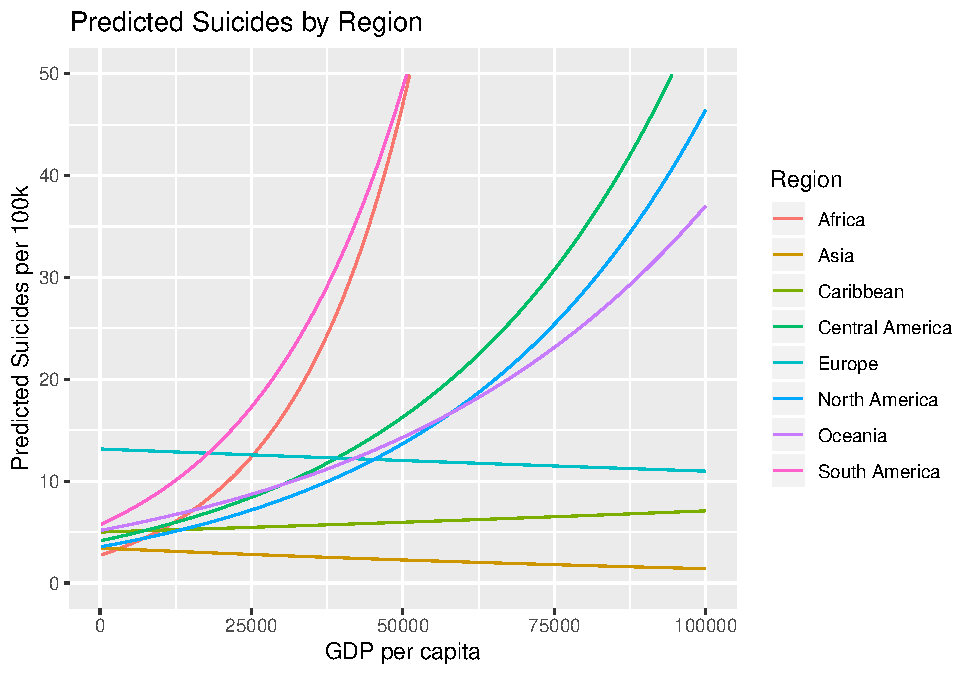
\includegraphics{An-Analysis-of-Suicide-Data_files/figure-latex/unnamed-chunk-15-1.pdf}





\newpage
\singlespacing 
\end{document}
